\begin{define}{Groups}[def:group][red]
  A nonempty set \(G\) is a \textbf{group} under the (binary) operation \(*\), 
  denoted \((G, *)\), if (and only if) these four propositions are satisfied:
  \begin{itemize}
    \item \textbf{Closure:} For all \(a, b \in G\), \(a * b \in G\).
    \item \textbf{Associativity:} For all \(a, b, c \in G\), \((a * b) * c = a * (b * c)\).
    \item \textbf{Existence of an identity:} There exists \(e \in G\) such that \(a * e = e * a = a\) for all \(a \in G\).
    \item \textbf{Existence of inverses:} For every \(a \in G\) there exists \(b \in G\) such that \(a * b = b * a = e\).
  \end{itemize}
\end{define}
\begin{enumerate}
  \item Prove that \((\setZ, +)\) is a \nameref{def:group}.
  \begin{subprove}
    Let \(G = \setZ\) and let the operation be \(+\).
    It will be proved that \((G, +)\) satisfies all four group properties.
    \begin{itemize}
      \item \textbf{Closure:} For any \(a, b \in G\), \(a + b \in G\) since the sum of two integers is an integer.
      \item \textbf{Associativity:} For any \(a, b, c \in G\), \((a + b) + c = a + (b + c)\) by the associativity of integer addition.
      \item \textbf{Existence of Identity:} The identity element is \(0\) since for any \(a \in G\), \(0 + a = a + 0 = a\).
      \item \textbf{Existence of Inverse:} For each \(a \in G\), the inverse element is \(-a\) since \(a + (-a) = (-a) + a = 0\).
    \end{itemize}
    Since all four group properties are satisfied, it follows that \((\setZ, +)\) is a \nameref{def:group}.
  \end{subprove}
  \item Prove that \((\setZ, \cdot)\) is not a \nameref{def:group}.
  \begin{subprove}
    Let \(G = \setZ\) and let the operation be \(\cdot\).
    It will be proved that \((G, \cdot)\) does not satisfy all four group properties.
    \begin{itemize}
      \item \textbf{Closure:} For any \(a, b \in G\), \(a \cdot b \in G\) since the product of two integers is an integer.
      \item \textbf{Associativity:} For any \(a, b, c \in G\), \((a \cdot b) \cdot c = a \cdot (b \cdot c)\) by the associativity of integer multiplication.
      \item \textbf{Existence of Identity:} The identity element is \(1\) since for any \(a \in G\), \(1 \cdot a = a \cdot 1 = a\).
      \item \textbf{Existence of Inverse:} For each \(a \in G\), there does not exist an inverse element \(a^{-1} \in G\) such that \(a \cdot a^{-1} = a^{-1} \cdot a = 1\) unless \(a = 1\) or \(a = -1\). For example, if \(a = 2\), then there is no integer \(b\) such that \(2 \cdot b = 1\).
    \end{itemize}
    Since the existence of inverse property is not satisfied for all elements in \(G\), it follows that \((\setZ, \cdot)\) is not a \nameref{def:group}.
  \end{subprove}
  \item Prove that \((\setQ, +)\) is a \nameref{def:group}.
  \begin{subprove}
    Let \(G = \setQ\) and let the operation be \(+\).
    It will be proved that \((G, +)\) satisfies all four group properties.
    \begin{itemize}
      \item \textbf{Closure:} For any \(a, b \in G\), \(a + b \in G\) since the sum of two rational numbers is a rational number.
      \item \textbf{Associativity:} For any \(a, b, c \in G\), \((a + b) + c = a + (b + c)\) by the associativity of rational number addition.
      \item \textbf{Existence of Identity:} The identity element is \(0\) since for any \(a \in G\), \(0 + a = a + 0 = a\).
      \item \textbf{Existence of Inverse:} For each \(a \in G\), the inverse element is \(-a\) since \(a + (-a) = (-a) + a = 0\).
    \end{itemize}
    Since all four group properties are satisfied, it follows that \((\setQ, +)\) is a \nameref{def:group}.
  \end{subprove}
  \item Prove that \((\setQ, \cdot)\) is not a \nameref{def:group}.
  \begin{subprove}
    Let \(G = \setQ\) and let the operation be \(\cdot\).
    It will be proved that \((G, \cdot)\) does not satisfy all four group properties.
    \begin{itemize}
      \item \textbf{Closure:} For any \(a, b \in G\), \(a \cdot b \in G\) since the product of two rational numbers is a rational number.
      \item \textbf{Associativity:} For any \(a, b, c \in G\), \((a \cdot b) \cdot c = a \cdot (b \cdot c)\) by the associativity of rational number multiplication.
      \item \textbf{Existence of Identity:} The identity element is \(1\) since for any \(a \in G\), \(1 \cdot a = a \cdot 1 = a\).
      \item \textbf{Existence of Inverse:} For each \(a \in G\), there does not exist an inverse element \(a^{-1} \in G\) such that \(a \cdot a^{-1} = a^{-1} \cdot a = 1\) if \(a = 0\). For example, if \(a = 0\), then there is no rational number \(b\) such that \(0 \cdot b = 1\).
    \end{itemize}
    Since the existence of inverse property is not satisfied for all elements in \(G\), it follows that \((\setQ, \cdot)\) is not a \nameref{def:group}.
  \end{subprove}
  \item Prove that \((\setQ^*, \cdot)\) is a \nameref{def:group}, where \(\setQ^* = \set{q \in \setQ \mid q \neq 0}\).
  \begin{subprove}
    Let \(G = \setQ^*\) and let the operation be \(\cdot\).
    It will be proved that \((G, \cdot)\) satisfies all four group properties.
    \begin{itemize}
      \item \textbf{Closure:} For any \(a, b \in G\), \(a \cdot b \in G\) since the product of two nonzero rational numbers is a nonzero rational number.
      \item \textbf{Associativity:} For any \(a, b, c \in G\), \((a \cdot b) \cdot c = a \cdot (b \cdot c)\) by the associativity of rational number multiplication.
      \item \textbf{Existence of Identity:} The identity element is \(1\) since for any \(a \in G\), \(1 \cdot a = a \cdot 1 = a\).
      \item \textbf{Existence of Inverse:} For each \(a \in G\), the inverse element is \(a^{-1} = \frac{1}{a}\) since \(a \cdot a^{-1} = a^{-1} \cdot a = 1\).
    \end{itemize}
    Since all four group properties are satisfied, it follows that \((\setQ^*, \cdot)\) is a \nameref{def:group}.
  \end{subprove}
  \item Prove that \((\setR^{+}, +)\) is not a \nameref{def:group}.
  \begin{subprove}
    Let \(G = \setR^{+}\) and let the operation be \(+\).
    It will be proved that \((G, +)\) does not satisfy all four group properties.
    \begin{itemize}
      \item \textbf{Closure:} For any \(a, b \in G\), \(a + b \in G\) since the sum of two positive real numbers is a positive real number.
      \item \textbf{Associativity:} For any \(a, b, c \in G\), \((a + b) + c = a + (b + c)\) by the associativity of real number addition.
      \item \textbf{Existence of Identity:} There does not exist an identity element \(e \in G\) such that for all \(a \in G\), \(e + a = a + e = a\) since the only candidate for the identity element is \(0\), which is not in \(G\).
      \item \textbf{Existence of Inverse:} For each \(a \in G\), there does not exist an inverse element \(a^{-1} \in G\) such that \(a + a^{-1} = a^{-1} + a = e\) since the only candidate for the inverse element is \(-a\), which is not in \(G\).
    \end{itemize}
    Since the existence of identity and existence of inverse properties are not satisfied, it follows that \((\setR^{+}, +)\) is not a \nameref{def:group}.
  \end{subprove}
  \item Prove that \((\setR^{+}, \cdot)\) is a \nameref{def:group}.
  \begin{subprove}
    Let \(G = \setR^{+}\) and let the operation be \(\cdot\).
    It will be proved that \((G, \cdot)\) satisfies all four group properties.
    \begin{itemize}
      \item \textbf{Closure:} For any \(a, b \in G\), \(a \cdot b \in G\) since the product of two positive real numbers is a positive real number.
      \item \textbf{Associativity:} For any \(a, b, c \in G\), \((a \cdot b) \cdot c = a \cdot (b \cdot c)\) by the associativity of real number multiplication.
      \item \textbf{Existence of Identity:} The identity element is \(1\) since for any \(a \in G\), \(1 \cdot a = a \cdot 1 = a\).
      \item \textbf{Existence of Inverse:} For each \(a \in G\), the inverse element is \(a^{-1} = \frac{1}{a}\) since \(a \cdot a^{-1} = a^{-1} \cdot a = 1\).
    \end{itemize}
    Since all four group properties are satisfied, it follows that \((\setR^{+}, \cdot)\) is a \nameref{def:group}.
  \end{subprove}
\end{enumerate}



\begin{define}{Abelian Groups}[def:abeliangroup][red]
  A \nameref{def:group} \((G, *)\) is called an \textbf{Abelian group} 
  (or \textbf{commutative group}) if (and only if) \textbf{commutative}, that is,
  \[
  \text{For all } a, b \in G, \, a * b = b * a.
  \]
\end{define}

\begin{enumerate}
  \item Let $G$ be a nonempty set of $2 \times 2$ matrices. 
  Then, $(G, \cdot)$ is not a \nameref{def:abeliangroup}, 
  where $\cdot$ is the matrix multiplication operation.
  \begin{subprove}
    Let \(G\) be the set of all \(2 \times 2\) matrices with real entries, and let the operation be matrix multiplication \(\cdot\).
    It will be proved that \((G, \cdot)\) does not satisfy the commutative property.
    The following two matrices in \(G\) are considered:
    \[
    A = \begin{pmatrix}
    1 & 2 \\
    0 & 1
    \end{pmatrix}, \quad
    B = \begin{pmatrix}
    1 & 0 \\
    3 & 1
    \end{pmatrix}.
    \]
    Now, \(A \cdot B\) and \(B \cdot A\) are computed:
    \[
    A \cdot B = \begin{pmatrix}
    1 & 2 \\
    0 & 1
    \end{pmatrix} \cdot \begin{pmatrix}
    1 & 0 \\
    3 & 1
    \end{pmatrix} = \begin{pmatrix}
    1 + 6 & 2 + 2 \\
    0 + 3 & 0 + 1
    \end{pmatrix} = \begin{pmatrix}
    7 & 4 \\
    3 & 1
    \end{pmatrix},
    \]
    and
    \[
    B \cdot A = \begin{pmatrix}
    1 & 0 \\
    3 & 1
    \end{pmatrix} \cdot \begin{pmatrix}
    1 & 2 \\
    0 & 1
    \end{pmatrix} = \begin{pmatrix}
    1 + 0 & 2 + 0 \\
    3 + 0 & 6 + 1
    \end{pmatrix} = \begin{pmatrix}
    1 & 2 \\
    3 & 7
    \end{pmatrix}.
    \]
    Since \(A \cdot B = \begin{pmatrix}
    7 & 4 \\ 
    3 & 1 
    \end{pmatrix}\) is not equal to \(B \cdot A = \begin{pmatrix}
    1 & 2 \\
    3 & 7
    \end{pmatrix}\).
    Therefore, \((G, \cdot)\) does not satisfy the commutative property, and hence it is not a \nameref{def:abeliangroup}.
  \end{subprove}
\end{enumerate}

\begin{define}{Finite Groups}[def:finitegroup][red]
  A \nameref{def:group} \((G, *)\) is called a \textbf{finite group} if (and only if) 
  the order of \(G\), denoted by \(|G|\), is finite; that is,
  \[
  |G| < \infty.
  \]
\end{define}



















\newpage
\begin{define}{Pigeonhole Principle}[def:pigeonhole][red]
  If \(k+1\) or more pigeons (objects) are placed into \(k\) pigeonholes (boxes), 
  then there is at least one pigeonhole (box) containing two or more pigeons (objects).
\end{define}
Let \(S\), \(T\), \(U\), and \(V\) be nonempty sets. 
\begin{enumerate}
  \item Let \(f: S \to T\), \(g: T \to U\), and \(h: U \to V\) be functions.
  Prove any of the following statements not already done before.
  \begin{enumerate}
    \item Prove that \(h \circ (g \circ f) = (h \circ g) \circ f\).
    \item Prove that \(i_{T} \circ f = f\) and \(f \circ i_{S} = f\).
    \item Prove that if \(f\) and \(g\) are bijective, then so is \(g \circ f\) directly from the definitions.
  \end{enumerate}
  \item Prove that a function \(f: S \to T\) is a bijection if and only if there exists a function \(g: T \to S\) with \(g \circ f = i_{S}\) and \(f \circ g = i_{T}\).
  \item The set of all one-to-one mappings from a nonempty set \(S\) onto itself is denoted \(A(S)\). 
  Prove that \(A(S)\) is a \nameref{def:group} under the operation of function composition. 
  For simplicity, write \(g \circ f\) as \(g f\) for \(f, g \in A(S)\).
  \item When \(|S| = n < \infty\), then \(A(S)\) is called the symmetric group of degree \(n\), often denoted \(S_{n}\). 
  The elements of \(S_{n}\) are called permutations of \(S\), and \(S_{n}\) has \(n!\) elements.
  Consider \(i, f, g \in S_{3}\) where \(i = \begin{pmatrix} 1 & 2 & 3 \\ 1 & 2 & 3 \end{pmatrix}\), 
  \(f = \begin{pmatrix} 1 & 2 & 3 \\ 2 & 1 & 3 \end{pmatrix}\), and \(g = \begin{pmatrix} 1 & 2 & 3 \\ 2 & 3 & 1 \end{pmatrix}\). 
  The notation means \(f(1) = 2\), \(f(2) = 1\), \(f(3) = 3\) while \(g(1) = 2\), \(g(2) = 3\), \(g(3) = 1\).
  \begin{enumerate}
    \item Prove that \(i, f, g, g^{2}, f g, g f\) are all distinct permutations by considering the symmetries of a triangle (under rotation and reflection) with vertices labeled 1, 2, and 3.
    \item Prove that \(f^{2} = f f = i\) and \(g^{3} = g(g^{2}) = i\). What are the inverses of the other elements?
    \item Complete the product table for \(S_{3}\) on the board:
    \begin{center}
    \begin{tabular}{|c|c|c|c|c|c|c|}
    \hline
    & \(i\) & \(f\) & \(g\) & \(g^{2}\) & \(f g\) & \(g f\) \\
    \hline
    \(i\) &  &  &  &  &  &  \\
    \hline
    \(f\) &  & \(i\) & \(f g\) &  &  &  \\
    \hline
    \(g\) &  & \(g f\) &  & \(i\) &  &  \\
    \hline
    \(g^{2}\) &  &  &  &  &  &  \\
    \hline
    \(f g\) &  &  &  &  &  &  \\
    \hline
    \(g f\) &  &  &  &  &  &  \\
    \hline
    \end{tabular}
    \end{center}
  \end{enumerate}
  \item Prove that if \(|S| \geq 3\), then \(A(S)\) is not a \nameref{def:abeliangroup}.
  \item Let \(f: S \to T\) and \(g: T \to U\) be functions.
  \begin{enumerate}
    \item Let \(h: T \to U\) be a function. Prove that if \(f\) is surjective and \(g \circ f = h \circ f\), then \(g = h\).
    \item Let \(h: S \to T\) be a function. Prove that if \(g\) is injective and \(g \circ f = g \circ h\), then \(f = h\).
  \end{enumerate}
  \item Let \(f: S \to S\) be a function.
  \begin{enumerate}
    \item Suppose \(S\) is finite. Prove that \(f\) is onto if and only if \(f\) is one-to-one.
    \item Disprove the general statement that \(f\) is onto only if \(f\) is one-to-one.
    \item Disprove the general statement that \(f\) is one-to-one only if \(f\) is onto.
  \end{enumerate}
\end{enumerate}






\newpage
You may assume that ( $\mathbb{Z},+$ ) is a group with identity 0 , and that multiplication on the integers is closed and associative with identity 1.\\
Also, the following number theory result may be used without proof.\\
If $a, b \in \mathbb{Z}$ with either $a \neq 0$ or $b \neq 0$, then the greatest common divisor of $a$ and $b$ is 1 if and only if there exist $n, m \in \mathbb{Z}$ such that $a n+b m=1$.
\begin{enumerate}
  \item Let $G$ be a group. (When not necessary for clarity the product $a * b$ is written as $a b$ for $a, b \in G$ and the group is denoted as simply $G$ instead of ( $G, *$ ).)\\
(a) Prove that if $a b=a c$, then $b=c$ for all $a, b, c \in G$.\\
(b) Prove that if $b a=c a$, then $b=c$ for all $a, b, c \in G$.
  \item Let $G$ be a group.\\
(a) Prove that $\left(a^{-1}\right)^{-1}=a$ for all $a \in G$.\\
"The inverse of the inverse of $a$ is $a$."\\
(b) Prove that $(a b)^{-1}=b^{-1} a^{-1}$ for all $a, b \in G$.\\
"The inverse of the product of $a$ and $b$ is the product of their inverses in reverse order."
  \item Fix an integer $n \geq 2$ and consider $\mathbb{Z}_{n}$, the integers modulo $n$.
\end{enumerate}
For example, $\mathbb{Z}_{3}=\{[0],[1],[2]\}=\{[-5],[9],[23]\}$, etc. Note, however, $\mathbb{Z}_{3} \neq\{0,1,2\}$ !\\
Define addition on $\mathbb{Z}_{n}$ as $[a]+[b]=[a+b]$ and multiplication as $[a] \cdot[b]=[a b]$ for all $[a],[b] \in \mathbb{Z}_{n}$.\\
(a) Prove that addition on $\mathbb{Z}_{n}$ is well-defined.

Hint: if $a \equiv a^{\prime}(\bmod n)$ and $b \equiv b(\bmod n)$, is $a+b \equiv a^{\prime}+b^{\prime}(\bmod n)$ ?\\
(b) Prove that multiplication on $\mathbb{Z}_{n}$ is also well-defined.\\
4. Prove that $\mathbb{Z}_{n}$ is a group under addition for any $n \geq 2$. Hint: read the directions.\\
5. Write out the product tables for ( $\mathbb{Z}_{n},+$ ) for $n=3,4,5,6$, and identify all their subgroups.\\
6. Write out the product tables for $\mathbb{Z}_{n}^{*}=\mathbb{Z}_{n} \backslash\{[0]\}$ under multiplication for $n=3,4,5,6$. Are these groups? Why (not)?\\
7. Prove that $\mathbb{Z}_{n}^{*}$ is a group under multiplication if and only if $n \geq 2$ is a prime. Hint: directions.




\newpage


Let $(G, *)$ be a group with identity $e$.\\
Exponent notation: For $a \in G$, define $a^{0}=e$. For $i \in \mathbb{Z}$ with $i \geq 1$, define $a^{i}=a * a^{i-1}$ and $a^{-i}=\left(a^{-1}\right)^{i}$. It follows that $a^{n} a^{m}=a^{n+m}$ and $\left(a^{n}\right)^{m}=a^{n m}$ for $n, m \in \mathbb{Z}$.

\begin{enumerate}
  \item Let $H \subseteq G$. Prove that ( $H, *$ ) is a subgroup of ( $G, *$ ) if and only if $H$ is nonempty, closed under the product of $G$, and contains inverses, i.e (1) $H \neq \emptyset$, (2) for all $a, b \in H, a * b \in H$, and (3) for all $a \in H, a^{-1} \in H$.
  \item Let $a \in G$ and consider the set $A=\left\{a^{i} \mid i \in \mathbb{Z}\right\}$. Prove that $A$ is a subgroup of $G$. This proves that (a), the cyclic subgroup generated by $a$, is well-defined.
  \item Consider the group of integers under addition. What is the cyclic subgroup generated by -1 ? What is (2)? Are the odd integers a subgroup of $(\mathbb{Z},+)$ ? Justify your answers.
  \item Does ( $\mathbb{Z}_{4},+$ ) have a proper cyclic subgroup? What about ( $\mathbb{Z}_{5},+$ )? Justify your answers.
  \item Consider the set $\mathbb{Z}_{2} \times \mathbb{Z}_{2}$ under the product of coordinate-wise addition. Prove this is a group. This group, denoted $V_{4}$, is called the Klein 4-group.
  \item A group $G$ is cyclic if there exists $a \in G$ such that $G=(a)$. Is ( $\mathbb{Z},+$ ) a cyclic group? What about ( $\mathbb{Z}_{n},+$ ) for integer $n>2$ ? Justify your answers.
  \item Prove that the Klein 4-group in problem 5 is abelian, but not cyclic.
  \item For each of the four group axioms, give an example of a set with a binary product for which the axiom fails.
  \item Give an example of a nonabelian group. Justify your answer fully, i.e. why is it a group and how is it nonabelian?
\end{enumerate}


\newpage


Let ( $G, *$ ) and ( $H, \circ$ ) be groups with identities $e \in G, f \in H$. Here $\circ$ is a generic product symbol (like $*$ ) and not function composition.\\
A function $\phi: G \rightarrow H$ is an isomorphism from $G$ onto $H$ if (1) $\phi$ is a bijection, and (2) $\phi(a * b)= \phi(a) \circ \phi(b)$ for all $a, b \in G$.\\
When proving an isomorphism, you should write the product symbol explicitly.

\begin{enumerate}
  \item Show that the groups $(\{-1,1\}, \cdot),\left(\mathbb{Z}_{2},+\right),\left(\mathbb{Z}_{3}^{*}, \cdot\right)$ are all pair-wise isomorphic.
  \item Prove or disprove:\\
(a) $\left(\mathbb{Z}_{5}^{*}, \cdot\right)$ is isomorphic to $\left(\mathbb{Z}_{4},+\right)$.\\
(b) $V_{4}$, the Klein 4-group, is isomorphic to to ( $\mathbb{Z}_{4},+$ ).\\
(c) ( $\mathbb{Z}_{6},+$ ) is isomorphic to $S_{3}$.
  \item Let $m>1$ be an integer and $H_{m}=\{m x \mid x \in \mathbb{Z}\}$. Prove that $H_{m}$ is a subgroup of ( $\mathbb{Z},+$ ).
  \item Let $G$ be a group with identity $e$ and $H=\left\{a \in G \mid a^{2}=e\right\}$.\\
(a) Prove that if $G$ is abelian, then $H$ is a subgroup of $G$.\\
(b) Is the statement true if $G$ is nonabelian? Justify your answer.
  \item Let $(G, *)$ be a group and $H$ a nonempty subset of $G$ that is closed under $*$.\\
(a) Prove that if $H$ is finite, then $H$ is a subgroup of $G$.\\
(b) Is $H$ a subgroup of $G$ if $G$ is finite? Justify your answer.\\
(c) What about if $G$ is infinite? Justify your answer.
  \item Up to isomorphism, how many groups of order $n$ are there for $n=1,2,3$ ? What about $n=4$ ? And $n=5$ ? Justify your answers with a product table.
  \item Consider the dihedral group of order 8: $D_{8}=<a, x \mid a^{2}=x^{4}=e, a x a^{-1}=x^{-1}>$. with identity $e$, generators $a$ and $x$, and relations $a^{2}=e, x^{4}=e$, and $a x a^{-1}=x^{-1}$.\\
(a) List all 10 subgroups of $D_{8}$.\\
(b) Which subgroups of $D_{8}$ are isomorphic to the Klein 4-group? Justify your answer.
\end{enumerate}



\newpage
Hint: Write one proof outline and then edit as needed.

\begin{enumerate}
  \item Find a formula for the following summations. Prove your formula is correct using induction.\\
(a) $1+2+3+\ldots+n$ for all integers $n \geq 1$.\\
(b) $1+2+2^{2}+\ldots+2^{n}$ for all nonnegative integers $n$.
  \item For which nonnegative integers $n$ do the following inequalities hold? Prove your answer is correct using mathematical induction.\\
(a) $2 n \leq n^{2}$\\
(b) $n^{2}<2^{n}$\\
(c) $2^{n} \leq n$ !\\
(d) $n!<n^{n}$
  \item Proof or spoof? Justify your answer.
\end{enumerate}

Claim: All horses are the same color. Proof: Let $P(n)$ be the proposition that all horses in a set of $n$ horses are the same color. Clearly, $P(1)$ is true. Now assume that $P(n)$ is true, so that all horses in any set of $n$ horses are the same color. Consider any $n+1$ horses; number these as horses $1,2,3, \ldots, n, n+1$. Now the first $n$ of these horses all must have the same color, and the last $n$ of these must also have the same color. Since the set of the first $n$ horses and the last $n$ horses overlap, all $n+1$ must be the same color. This shows that $P(n+1)$ is true and finishes the proof by induction.\\
4. Prove that $n^{2}-1$ is divisible by 8 whenever $n$ is an odd positive integer.\\
5. (a) Determine which amounts of postage can be formed using just 5 -cent and 6 -cent stamps.\\
(b) Prove your answer is correct using mathematical induction.\\
(c) Prove your answer is correct using the "strong" form of mathematical induction.\\
6. Let $h$ be a real number with $h>-1$. Prove that $1+n h \leq(1+h)^{n}$ for all $n \mathbb{Z}, n>0$. This is called Bernoulli's inequality.\\
7. Fix $a, r \in \mathbb{R}$. A geometric progression is an infinite sequence of the form $a, a r, a r^{2}, \ldots, a r^{n}, \ldots$. Find a formula for the sum of the first $n$ terms of a geometric progression, and prove it is correct using induction.

\newpage

\begin{enumerate}
  \item Let $h$ be a real number with $h>-1$. Prove that $1+n h \leq(1+h)^{n}$ for all $n \in \mathbb{Z}, n>0$. This is called Bernoulli's inequality.
  \item Fix $a, r \in \mathbb{R}$. A geometric progression is an infinite sequence of the form $a, a r, a r^{2}, \ldots, a r^{n}, \ldots$. Find a formula for the sum of the first $n$ terms of a geometric progression, and prove it is correct using induction.
  \item Prove by induction that a set having $n$ elements has exactly $2^{n}$ subsets.
  \item Prove by induction on $k$ that a set of size $n$ has exactly $\binom{n}{k}$ subsets of size $k$ where $\binom{n}{k}= \frac{n!}{k!(n-k)!}$.
  \item Let $m>1$ be an integer and $H_{m}=\{m x \mid x \in \mathbb{Z}\}$. Prove that $H_{m}$ is a subgroup of ( $\mathbb{Z},+$ ).
  \item Let $G$ be a group with identity $e$ and $H=\left\{a \in G \mid a^{2}=e\right\}$.\\
(a) Prove that if $G$ is abelian, then $H$ is a subgroup of $G$.\\
(b) Is the statement true if $G$ is nonabelian? Justify your answer.
  \item Let ( $G, *$ ) be a group and $H$ a nonempty subset of $G$ that is closed under *.\\
(a) Prove that if $H$ is finite, then $H$ is a subgroup of $G$.\\
(b) Is $H$ a subgroup of $G$ if $G$ is finite? Justify your answer.\\
(c) What about if $G$ is infinite? Justify your answer.
\end{enumerate}







\newpage


\begin{enumerate}
  \item Choose one (or more) problems from an ICA and/or Webwork and/or Homework to work on as a group, or work on some of the problems below.
  \item Let ( $G, *$ ) and ( $H, \circ$ ) be two groups. Prove that if $\phi: G \rightarrow H$ is an isomorphism, then the inverse function $\phi^{-1}$ is an isomorphism from $H$ to $G$.
  \item Let $G, H$, and $K$ be three groups. Prove that if $\phi: G \rightarrow H$ and $\psi: H \rightarrow K$ are isomorphisms, then the composition $\psi \circ \phi: G \rightarrow K$ is an isomorphism.
  \item Let $\mathcal{G}$ be the set of all groups. Define a relation on $\mathcal{G}$ where $G \simeq G^{\prime}$ if and only if $G$ is isomorphic to $G^{\prime}$ for all $G, G^{\prime} \in \mathcal{G}$. Prove that this is an equivalence relation.
  \item Let $m$ be a positive integer. Prove that if $a$ and $b$ are integers with $a \equiv b(\bmod m)$, then $a^{k} \equiv b^{k}(\bmod m)$ whenever $k$ is a nonnegative integer.
  \item Let $G$ be a set with an operation * such that:
\end{enumerate}

\begin{itemize}
  \item $G$ is closed under *.
  \item * is associative.
  \item There exists an element $e \in G$ such that $e * x=x$ for all $x \in G$.
  \item Given $x \in G$, there exists a $y \in G$ such that $y * x=e$.
\end{itemize}

Prove that $G$ is a group.\\
Hint: first show that the left inverse of $x$ is also a right inverse using its own left inverse.
















































\begin{define}{Group}[def:group-recap][red]
  A nonempty set \(G\) with a binary operation \(*: G \times G \to G\), written \((G, *)\), is a \textbf{group} if and only if
  \begin{itemize}
    \item \textbf{Closure:} For all \(a,b \in G\), \(a * b \in G\).
    \item \textbf{Associativity:} For all \(a,b,c \in G\), \((a * b) * c = a * (b * c)\).
    \item \textbf{Identity:} There exists \(e \in G\) such that for all \(a \in G\), \(e * a = a * e = a\).
    \item \textbf{Inverses:} For each \(a \in G\) there exists \(b \in G\) such that \(a * b = b * a = e\).
  \end{itemize}
\end{define}

Groups are generalizations of the familiar products of addition and of multiplication of real numbers. Remember, though, that a set with a product is a group if and only if the four axioms are satisfied!

For instance, $\setZ$ is a group under addition but not under multiplication (for more than one reason). The set $\mathbb{Q}$ is also group under addition but not under multiplication. The set $\mathbb{R}^{+}$of positive real numbers is a group under multiplication but not under addition.

The groups above are infinite, but many interesting groups are finite. The order of a group $G$ is the number of elements in $G$, denoted $|\boldsymbol{G}|$. If (and only if) $|\boldsymbol{G}|<\infty$, then $G$ is a finite group.

The smallest group consists of a single (identity) element, usually denoted $e$ (or sometimes $i$ when the group elements are functions).
Here's an example of a group of order 2:
Claim: The set $\{-1,1\}$ under multiplication is a group.
Proof: Consider the set $\{-1,1\}$ under multiplication, denoted $\cdot$. Since $-1 \cdot-1=1=1 \cdot 1$ and $-1 \cdot 1=-1=1 \cdot-1$, then $\{-1,1\}$ is closed under multiplication. Since multiplication of real number is associative, then multiplication on $\{-1,1\}$ is associative. Since $-1 \cdot 1=1 \cdot-1=-1$ and $1 \cdot 1=1$, then 1 is the identity under multiplication. Since $-1 \cdot-1=1$ and $1 \cdot 1=1$, then both -1 and 1 have multiplicative inverses. Since all four axioms are satisfied, $(\{-1,1\}, \cdot)$ is a group. QED

When the order of a group is small, it is often very useful to write out the product table for the group.


For instance, let $G$ be a group of order two with product $*$. Then $G=\{e, a\}$ where $e$ is the identity and $a$ denotes the single non-identity element. The product table for $G$ is:

\begin{tabular}{|l|l|l|}
\hline$*$ & $e$ & $a$ \\
\hline$e$ & $e$ & $a$ \\
\hline$a$ & $a$ & $e$ \\
\hline
\end{tabular}

This is the "only" group of order 2. By which we mean that all groups of order 2 must be isomorphic to this group.
\begin{define}{Group Isomorphism}[def:group-isomorphism][red]
  Let \((G, *)\) and \((G', \star)\) be groups. An \textbf{isomorphism} is a bijection \(\phi: G \to G'\) such that \(\phi(a * b) = \phi(a) \star \phi(b)\) for all \(a,b \in G\). We write \(G \simeq G'\) if such a map exists.
\end{define}

Claim: The group $(\{-1,1\}, \cdot)$ is isomorphic to the group $(G, *)$ with product table above.
Proof: Let $\phi:\{-1,1\} \rightarrow\{e, a\}$ be the function given by $\phi(1)=e$ and $\phi(-1)=a$. Then by inspection $\phi$ is one-to-one and onto, and hence a bijection. Also, $\phi(1 \cdot 1)=\phi(1)=e=e * e=\phi(1) * \phi(1)$, $\phi(1 \cdot-1)=\phi(-1)=a=e * a=\phi(1) * \phi(-1)$, $\phi(-1 \cdot 1)=\phi(-1)=a=a * e=\phi(-1) * \phi(1)$, and $\phi(-1 \cdot-1)=\phi(1)=e=a * a=\phi(-1) * \phi(-1)$.
Hence, $\phi$ preserve operations, and $(\{-1,1\}, \cdot) \simeq(\{e, a\}, *)$. QED
Can you think of another group of order 2 ? What about the set $\left\{[0]_2,[1]_2\right\}$ of congrunence classes modulo two under addition? Can you prove this is isomorphic to $(G, *)$ with product table above?

Fill in the product tables below. Let $e$ denote the identity element.
Hint: How many times can an element appear in a given row (or column)? How many times must an element appear in a given row (or column)? If $g * h=h$ in a group $(G, *)$ with $g, h \in G$, then what is known about $g$ ?


Up to isomorphism, there is one group of order 3. You should understand why after filling in this product table.

\begin{tabular}{|c|c|c|c|}
\hline & $e$ & $a$ & $b$ \\
\hline$e$ & & & \\
\hline$a$ & & & \\
\hline$b$ & & & \\
\hline
\end{tabular}

Up to isomorphism, there are two groups of order 4. Identify the first one by completing this product table.

\begin{tabular}{|c|c|c|c|c|}
\hline & $e$ & $a$ & $b$ & $c$ \\
\hline$e$ & & & & \\
\hline$a$ & & $b$ & & \\
\hline$b$ & & & & \\
\hline$c$ & & & & \\
\hline
\end{tabular}

Identify the other group of order 4 which is not isomorphic to the previous one.
Hint: confirm your answer is not isomorphic to the previous group of order 4 under bijections like $b \leftrightarrow c$ or $a \leftrightarrow b$.

\begin{tabular}{|c|c|c|c|c|}
\hline & $e$ & $a$ & $b$ & $c$ \\
\hline$e$ & & & & \\
\hline$a$ & & & & \\
\hline$b$ & & & & \\
\hline$c$ & & & & \\
\hline$c$ & & & & \\
\hline
\end{tabular}





\newpage


Recall Wbwk8, Problem 4.
Fix $n \geq 2$ and consider $\setZ_n$, the set of equivalence classes under the relation congruence modulo $n$ on $\setZ$.
Are the following propositions true or false?

\begin{enumerate}
  \item Since addition on $\setZ$ is associative, so is addition on $\setZ_n$.
  \item Since multiplication on $\setZ$ is commutative, so is multiplication on $\setZ_n$.
  \item For all $a, b, c, d \in \setZ$, if $[a]=[b]$ and $[c]=[d]$, then $[a c]=[b d]$.
  \item Multiplication is well-defined on $\setZ_n$.
  \item Since multiplication on $\setZ$ is associative, so is multiplication on $\setZ_n$.
  \item Addition is well-defined on $\setZ_n$.
  \item For all $a, b, c, d \in \setZ$, if $[a]=[b]$ and $[c]=[d]$, then $[a+c]=[b+d]$.
  \item Since addition on $\setZ$ is commutative, so is addition on $\setZ_n$.
\end{enumerate}

Now, compute the following sum and product tables for $n=6$.

\begin{tabular}{|l|l|l|l|l|l|l|}
\hline+ & {$[0]$} & {$[1]$} & {$[2]$} & {$[3]$} & {$[4]$} & {$[5]$} \\
\hline$[0]$ & & & & & & \\
\hline$[1]$ & & & & & & \\
\hline$[2]$ & & & & & & \\
\hline$[3]$ & & & & & & \\
\hline$[4]$ & & & & & & \\
\hline$[5]$ & & & & & & \\
\hline
\end{tabular}

\begin{tabular}{|c|c|c|c|c|c|c|}
\hline. & {$[0]$} & {$[1]$} & {$[2]$} & {$[3]$} & {$[4]$} & {$[5]$} \\
\hline$[0]$ & & & & & & \\
\hline$[1]$ & & & & & & \\
\hline$[2]$ & & & & & & \\
\hline$[3]$ & & & & & & \\
\hline$[4]$ & & & & & & \\
\hline$[5]$ & & & & & & \\
\hline
\end{tabular}





\newpage


Fix $n \geq 2$ and consider $\setZ_n$, the set of equivalence classes under the relation congruence modulo $n$ on $\setZ$.
By definition, $\setZ_n^*=\setZ_n \backslash\{[0]\}$.
Are the following propositions true or false?



\begin{itemize}
  \item[(\textbf{false})] Under multiplication $[0]$ is the identity element in $\setZ_n$.
  \item[(\textbf{false})] The set $\setZ_n$ is a group under the product of multiplication.
  \item[(\textbf{true})] There exists an identity element in $\setZ_n$ under addition.
  \item[(\textbf{false})] The set $\setZ_n^*$ is a group under the product of multiplication.
  \item[(\textbf{false})] For every $[a] \in \setZ_n$ there exists a $[b] \in \setZ_n$ such that $[a b]$ is the multiplicative identity.
  \item[(\textbf{true})] Under multiplication $[1]$ is the identity element in $\setZ_n^*$.
  \item[(\textbf{false})] Under multiplication $[0]$ is the identity element in $\setZ_n^*$ when $n$ is prime.
  \item[(\textbf{true})] Under addition $[0]$ is the identity element in $\setZ_n$.
  \item[(\textbf{true})] There exist inverses in $\setZ_n^*$ under multiplication when $n$ is prime.
  \item[(\textbf{true})] There exists an identity element in $\setZ_n^*$ under multiplication.
  \item[(\textbf{true})] The set $\setZ_n^*$ is a group under the product of multiplication when $n$ is prime.
  \item[(\textbf{false})] For every $[a] \in \setZ_n^*$ there exists a $[b] \in \setZ_n^*$ such that $[a b]$ is the multiplicative identity.
  \item[(\textbf{true})] For every $[a] \in \setZ_n$ there exists a $[b] \in \setZ_n$ such that $[a+b]$ is the additive identity.
  \item[(\textbf{true})] Under multiplication $[1]$ is the identity element in $\setZ_n^*$ when $n$ is prime.
  \item[(\textbf{true})] There exists an identity element in $\setZ_n$ under multiplication.
  \item[(\textbf{false})] There exist inverses in $\setZ_n$ under multiplication.
  \item[(\textbf{false})] Under multiplication $[0]$ is the identity element in $\setZ_n^*$.
  \item[(\textbf{true})] For every $[a] \in \setZ_n^*$ there exists a $[b] \in \setZ_n^*$ such that $[a b]$ is the multiplicative identity when $n$ is prime.
  \item[(\textbf{false})] Under addition $[1]$ is the identity element in $\setZ_n$.
  \item[(\textbf{true})] The set $\setZ_n$ is a group under the product of addition.
  \item[(\textbf{true})] Under multiplication $[1]$ is the identity element in $\setZ_n$.
  \item[(\textbf{true})] There exists an identity element in $\setZ_n^*$ under multiplication when $n$ is prime.
  \item[(\textbf{true})] There exist inverses in $\setZ_n$ under addition.
  \item[(\textbf{false})] There exist inverses in $\setZ_n^*$ under multiplication.
\end{itemize}





\newpage

\begin{define}{Nonabelian Group: Symmetries of an Equilateral Triangle}[def:nonabelian-triangle][red]
A group $(G, *)$ is \textbf{abelian} if and only if $a * b = b * a$ for all $a, b \in G$.
While many familiar groups are abelian, most groups are not! Hence, it is very important to understand well some examples of nonabelian groups.

The smallest nonabelian group has order 6. One way to understand this group is as the symmetries of an equilateral triangle.

Consider an equilateral triangle with vertex labels $1$, $2$, and $3$:

\begin{center}
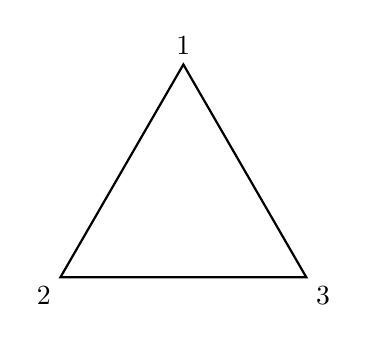
\begin{tikzpicture}[scale=1.2]
  % Vertices
  \coordinate (A) at (0,1.5);
  \coordinate (B) at (-1.3,-0.75);
  \coordinate (C) at (1.3,-0.75);
  \coordinate (O) at (0,0);

  % Triangle
  \draw[thick] (A) -- (B) -- (C) -- cycle;

  % Vertex labels
  \node[above] at (A) {1};
  \node[below left] at (B) {2};
  \node[below right] at (C) {3};

  % Center
  \coordinate (O) at (0,0);
\end{tikzpicture}
\end{center}

Let $f$ be a reflection through the vertical axis. So $f$ fixes point $1$ and switches $2$ and $3$.

Let $g$ be a rotation $120^\circ$ clockwise around the center point. So $g$ sends $1$ to $2$, $2$ to $3$, and $3$ to $1$.

There are four other symmetries of an equilateral triangle. What are they in terms of either an axis of reflection or an angle of rotation?

The composition of two symmetries is another symmetry, and this product is associative. There is an identity symmetry, and every symmetry has an inverse. Why? How would you justify these statements?

Hence, the symmetries of an equilateral triangle form a group under composition.
\end{define}

Match each symmetry on the left with an equivalent one from the right if possible. The notation $fg$ means $f \circ g$, so first rotate $120^\circ$, then reflect through the vertical axis.
\begin{enumerate}[label=\Alph*.]
  \item $g f$
  \item $g^{-1}$
  \item $g^2 f$
  \item $f$
  \item $f^2$
  \item None of the above
\end{enumerate}

Match the following.
\begin{enumerate}
  \item $f^{-1}$
  \item $g^3$
  \item $f g^2$
  \item $f g$
  \item $g^2$
\end{enumerate}


Fill in the product table below using the given labels for the symmetries. Let $e$ denote the identity symmetry. Enter $g^2$ as "gg" and $f g^2$ as "fgg".

\begin{tabular}{|c|c|c|c|c|c|c|}
\hline & $e$ & $f$ & $g$ & $g^2$ & $f g$ & $f g^2$ \\
\hline$e$ & & & & & & \\
\hline$f$ & & & & & \\
\hline$g$ & & & & & & \\
\hline$g^2$ & & & & & & \\
\hline$f g$ & & & & & & \\
\hline$f g^2$ & & & & & & \\
\hline
\end{tabular}


\begin{define}{Order of an Element}[def:order-element][red]
  Let \((G, *)\) be a group with identity \(e\). The \textbf{order} of an element \(a \in G\), denoted \(o(a)\), is the least positive integer \(m\) such that \(a^{m} = e\). If no such \(m\) exists, we say \(a\) has \textbf{infinite order}.
\end{define}

Let $(G, *)$ be the group of symmetries of an equilateral triangle under composition. What are the truth values of the following propositions?
\begin{enumerate}
  \item Every element in $(G, *)$ has order 2 or 3.
  \item $f g = g^{-1} f$ but $g \neq g^{-1}$.
  \item The order of $(G, *)$ is 6.
  \item The order of $g^2$ is 6.
  \item The order of $f$ is 2.
  \item $(f g)^2 \neq f^2 g^2$.
  \item For all elements $h \in G$, $h^6 = e$.
  \item The order of $g$ is 3.
  \item The order of every element in $(G, *)$ divides the order of the group.
  \item $g^2 (f g) = (f g) g^2$.
  \item $(G, *)$ is an abelian group.
\end{enumerate}




\newpage



Up to isomorphism, there is a unique group of order 5 . Let $G=\{a, b, c, d, e\}$ be a group with product *. Complete the product table for $(G, *)$ below.

\begin{center}
  \begin{tabular}{|l|c|c|c|c|c|}
  \hline$*$ & $e$ & $a$ & $b$ & $c$ & $d$ \\
  \hline$e$ & $e$ & $a$ & $b$ & $c$ & $d$ \\
  \hline$a$ & $a$ & $b$ & $d$ & $e$ & $c$ \\
  \hline$b$ & $b$ & $d$ & $c$ & $a$ & $e$ \\
  \hline$c$ & $c$ & $e$ & $a$ & $d$ & $b$ \\
  \hline$d$ & $d$ & $c$ & $e$ & $b$ & $a$ \\
  \hline
  \end{tabular}
\end{center}


The congruence classes modulo 5 are also a group of order 5 under addition. Show that ( $\setZ_5,+$ ) is isomorphic to $(G, *)$ in several different ways by completing the various bijections $\phi: \setZ_5 \rightarrow G$ below.

Match the elements of $\setZ_5$ on the left with their images in $G$. Remember that the bijection $\phi$ must preserve operations to be an isomorphism.


\begin{enumerate}
  \item Suppose $\phi$ maps $[1]$ to $a$.
  \begin{subanswer}
    \begin{itemize}
      \item $\phi([0]) \rightarrow e$
      \item $\phi([1]) \rightarrow a$
      \item $\phi([2]) \rightarrow a^2 = b$
      \item $\phi([3]) \rightarrow a^3 = d$
      \item $\phi([4]) \rightarrow a^4 = c$
    \end{itemize}
  \end{subanswer}
  \item Suppose $\phi$ maps $[1]$ to $b$.
  \begin{subanswer}
    \begin{itemize}
      \item $\phi([0]) \rightarrow e$
      \item $\phi([1]) \rightarrow b$
      \item $\phi([2]) \rightarrow b^2 = c$
      \item $\phi([3]) \rightarrow b^3 = a$
      \item $\phi([4]) \rightarrow b^4 = d$
    \end{itemize}
  \end{subanswer}
  
  \item Suppose $\phi$ maps $[1]$ to $c$.
  \begin{subanswer}
    \begin{itemize}
      \item $\phi([0]) \rightarrow e$
      \item $\phi([1]) \rightarrow c$
      \item $\phi([2]) \rightarrow c^2 = d$
      \item $\phi([3]) \rightarrow c^3 = b$
      \item $\phi([4]) \rightarrow c^4 = a$
    \end{itemize}
  \end{subanswer}
  \item Suppose $\phi$ maps $[1]$ to $d$.
  \begin{subanswer}
    \begin{itemize}
      \item $\phi([0]) \rightarrow e$ \hfill (identity: $d^0 = e$)
      \item $\phi([1]) \rightarrow d$ \hfill ($d^1 = d$)
      \item $\phi([2]) \rightarrow d^2 = a$ \hfill ($d^2 = a$ from the table)
      \item $\phi([3]) \rightarrow d^3 = c$ \hfill ($d^3 = c$ from the table)
      \item $\phi([4]) \rightarrow d^4 = b$ \hfill ($d^4 = b$ from the table)
    \end{itemize}
  \end{subanswer}
  \item Suppose $\phi$ maps $[2]$ to $a$.
  \begin{subanswer}
    \begin{itemize}
      \item $\phi([0]) \rightarrow e$ \hfill (identity: $a^0 = e$)
      \item $\phi([1]) \rightarrow d$ \hfill ($a^1 = a$, but $a = d^2$, so $d$ is the element after $e$ in the cycle)
      \item $\phi([2]) \rightarrow a$ \hfill (by assumption)
      \item $\phi([3]) \rightarrow c$ \hfill ($a^3 = c$ from the table)
      \item $\phi([4]) \rightarrow b$ \hfill ($a^4 = b$ from the table)
    \end{itemize}
  \end{subanswer}
  \item Suppose $\phi$ maps $[3]$ to $a$.
  \begin{subanswer}
    \begin{itemize}
      \item $\phi([0]) \rightarrow e$ \hfill (identity: $a^0 = e$)
      \item $\phi([1]) \rightarrow b$ \hfill ($a^1 = a$, $a^2 = b$)
      \item $\phi([2]) \rightarrow c$ \hfill ($a^3 = c$)
      \item $\phi([3]) \rightarrow a$ \hfill (by assumption)
      \item $\phi([4]) \rightarrow d$ \hfill ($a^4 = d$)
    \end{itemize}
  \end{subanswer}
  \item Suppose $\phi$ maps $[4]$ to $a$.
  \begin{subanswer}
    \begin{itemize}
      \item $\phi([0]) \rightarrow e$
      \item $\phi([1]) \rightarrow c$
      \item $\phi([2]) \rightarrow d$
      \item $\phi([3]) \rightarrow b$
      \item $\phi([4]) \rightarrow a$
    \end{itemize}
  \end{subanswer}
\end{enumerate}







\newpage


\begin{define}{Subgroup}[def:subgroup][red]
  A nonempty subset $H$ of $G$ is called a subgroup of $G$ if (and only if) $H$ itself is a group under the product of $G$.
\end{define}


\begin{define}{Subgroup Lemma}[def:subgroup-lemma][red]
  A subset $A \subseteq G$ is a subgroup of $\group{G, *}$ if and only if 
  \begin{enumerate}
    \item $A$ is nonempty,
    \item for all $a, b \in A, a * b \in A$, and
    \item for all $a \in A, a^{-1} \in A$
  \end{enumerate}
\end{define}

Select all subgroups of the group $\setZ_5$ under addition.
\begin{enumerate}
  \item $\{[1]\}$
  \item $\{[0],[2],[4]\}$
  \item $\{[0],[1],[4]\}$
  \item $\{[0],[3]\}$
  \item $\{[1],[2],[3]\}$
  \item $\{[0],[1],[3]\}$
  \item $\{[0],[1]\}$
  \item $\{[0],[1],[2],[3],[4]\}$
  \item $\{[0]\}$
  \item $\{[1],[2],[3],[4]\}$
\end{enumerate}
\begin{subanswer}
  I, H (i.e. $\{[0]\},\ \setZ_5$).
\end{subanswer}

Select all subgroups of the group \(\setZ_6\) under addition.
\begin{enumerate}[label=\Alph*.]
  \item $\{[2],[4]\}$
  \item $\{[0]\}$
  \item $\{[1],[2],[3],[4],[5]\}$
  \item $\{[0],[2],[4]\}$
  \item $\{[0],[2],[3],[4]\}$
  \item $\{[0],[1],[3],[5]\}$
  \item $\{[1]\}$
  \item $\{[0],[1],[2],[3],[4],[5]\}$
  \item $\{[3]\}$
  \item $\{[0],[3]\}$
\end{enumerate}
\begin{subanswer}
  B, D, J, H (i.e. $\{[0]\},\ \{[0],[2],[4]\},\ \{[0],[3]\},\ \setZ_6$).
\end{subanswer}

Select all subgroups of the group \(\setZ_5^*\) under multiplication.
\begin{enumerate}[label=\Alph*.]
  \item $\{[0],[1],[2],[3],[4]\}$
  \item $\{[1]\}$
  \item $\{[0]\}$
  \item $\{[3]\}$
  \item $\{[2],[4]\}$
  \item $\{[1],[4]\}$
  \item $\{[2],[3],[4]\}$
  \item $\{[0],[1],[3]\}$
  \item $\{[1],[3]\}$
  \item $\{[1],[2],[3],[4]\}$
\end{enumerate}
\begin{subanswer}
  B, F, J (i.e. $\{[1]\},\ \{[1],[4]\},\ \setZ_5^*$).
\end{subanswer}



\newpage

As you know from Webwork 10, Problem 1, there are two non-isomorphic groups of order 4. The second one from that problem is named the \textbf{Klein 4-group} and denoted $V_4$.

$V_4$ has the group presentation $< a, b \mid a^2 = e, b^2 = e, (ab)^2 = e >$ where $e$ is the identity element. Hence, the elements $a$ and $b$ generate the group under the relations $a^2 = e$, $b^2 = e$, and $(ab)^2 = e$.

Match each element on the left with an equivalent one from the right if possible.

\vspace{1em}
\noindent\textbf{Elements to Match:}
\begin{enumerate}
  \item $aba$
  \item $a^{-1}$
  \item $(ab)^{-1}$
  \item $ba$
  \item $b^{-1}$
  \item $bab$
\end{enumerate}

\noindent\textbf{Options:}
\begin{enumerate}[label=\Alph*.]
  \item $a$
  \item $ab$
  \item $b$
  \item None of the above
\end{enumerate}

\begin{subanswer}
The given relations imply several key properties:
\begin{itemize}
  \item $a^2 = e \implies a^{-1} = a$.
  \item $b^2 = e \implies b^{-1} = b$.
  \item $(ab)^2 = e \implies (ab)^{-1} = ab$.
  \item The relations also imply the group is abelian: $(ab)(ab) = e$. Multiplying on the left by $a$ gives $a(abab) = ae \implies (a^2)bab = a \implies bab = a$. Multiplying this on the right by $b$ gives $(bab)b = ab \implies ba(b^2) = ab \implies ba = ab$.
\end{itemize}
Using these properties, we can simplify each expression:
\begin{itemize}[itemsep=0pt, topsep=0pt]
  \item 1. $aba = a(ba) = a(ab) = (a^2)b = eb = b \quad \to \quad \textbf{C}$
  \item 2. $a^{-1} = a \quad \to \quad \textbf{A}$
  \item 3. $(ab)^{-1} = ab \quad \to \quad \textbf{B}$
  \item 4. $ba = ab \quad \to \quad \textbf{B}$
  \item 5. $b^{-1} = b \quad \to \quad \textbf{C}$
  \item 6. $bab = (ba)b = (ab)b = a(b^2) = ae = a \quad \to \quad \textbf{A}$
\end{itemize}
\end{subanswer}



\newpage


Fill in the product table below using the given labels for the elements.
\vspace{1em}

\begin{center}
% The Klein 4-group V_4 is abelian, with every non-identity element
% having order 2. The table is derived from these properties.
\begin{tabular}{|c||c|c|c|c|}
\hline
$\circ$ & $e$ & $a$ & $b$ & $ab$ \\
\hline\hline
$e$ & $e$ & $a$ & $b$ & $ab$ \\
\hline
$a$ & $a$ & $e$ & $ab$ & $b$ \\
\hline
$b$ & $b$ & $ab$ & $e$ & $a$ \\
\hline
$ab$ & $ab$ & $b$ & $a$ & $e$ \\
\hline
\end{tabular}
\end{center}

\vspace{2em}
Select all subgroups of Klein 4-group.

\begin{enumerate}[label=\Alph*.]
  \item $\{e, b, ab\}$
  \item $\{e, a\}$
  \item $\{e\}$
  \item $\{\}$
  \item $\{a, b, ab\}$
  \item $\{e, b\}$
  \item $\{b, ab\}$
  \item $\{a, b\}$
  \item $\{e, a, ab\}$
  \item $\{a, ab\}$
  \item $\{a\}$
  \item $\{b\}$
  \item $\{e, a, b\}$
  \item $\{e, a, b, ab\}$
  \item $\{e, ab\}$
  \item $\{ab\}$
\end{enumerate}

\begin{subanswer}
To be a subgroup, a subset must contain the identity element $e$, be closed under the operation, and contain the inverse of each of its elements.
\begin{itemize}
    \item Options D, E, G, H, J, K, L, P fail because they do not contain the identity $e$.
    \item Options A, I, M fail the closure property (e.g., in A, $b \circ ab = a$, which is not in the set).
\end{itemize}
The correct options are: \textbf{B, C, F, N, O} \\
(i.e., $\{e, a\}$, $\{e\}$, $\{e, b\}$, $\{e, a, b, ab\}$, and $\{e, ab\}$).
\end{subanswer}





\newpage






\section*{Problem 1: $(\mathbb{Z}_4, +)$ vs. $V_4$}

To demonstrate that two groups are not isomorphic, one must find a characteristic which is different between the groups. Select all characteristics which could be used to show that $V_4$ is not isomorphic to $(\mathbb{Z}_4, +)$.

\begin{enumerate}[label=\Alph*.]
  \item $(\mathbb{Z}_4, +)$ has an element of order 4 but $V_4$ does not.
  \item Every element of $V_4$ is its own inverse, but $[1],[3] \in \mathbb{Z}_4$ with $[1]^{-1} = [3]$ and $[3]^{-1} = [1]$.
  \item $(\mathbb{Z}_4, +)$ has an element of order 1 but $V_4$ does not.
  \item $V_4$ has a subgroup of order 1 but $(\mathbb{Z}_4, +)$ does not.
  \item $V_4$ has an element of order 2 but $V_4$ does not.
  \item $(\mathbb{Z}_4, +)$ is abelian but $V_4$ is not.
  \item $(\mathbb{Z}_4, +)$ has one element of order 2 while $V_4$ has three.
  \item $V_4$ has a subgroup of order 4 but $(\mathbb{Z}_4, +)$ does not.
  \item $V_4$ is cyclic but $(\mathbb{Z}_4, +)$ is not. See problem 5.
  \item $V_4$ has a subgroup of order 2 but $(\mathbb{Z}_4, +)$ does not.
  \item $V_4$ has three subgroups of order 2 while $(\mathbb{Z}_4, +)$ only has one.
  \item $(\mathbb{Z}_4, +)$ is cyclic but $V_4$ is not. See problem 5.
  \item $V_4$ is abelian but $(\mathbb{Z}_4, +)$ is not.
  \item None of the above
\end{enumerate}

\begin{subanswer}
  The correct statements that distinguish the two groups are \textbf{A, B, G, K, L}.
  \begin{itemize}
    \item \textbf{A}: True. $(\mathbb{Z}_4, +)$ has elements [1] and [3] of order 4. All non-identity elements in $V_4$ have order 2.
    \item \textbf{B}: True. This is a restatement of the order property. In $V_4$, $x^2=e$ for all $x$, so $x=x^{-1}$. In $\mathbb{Z}_4$, $[1]^{-1}=[3]$.
    \item \textbf{C}: False. Both groups have an identity element of order 1.
    \item \textbf{D}: False. Both groups have a trivial subgroup $\{e\}$ (or $\{[0]\}$) of order 1.
    \item \textbf{E}: False. Both groups have elements of order 2.
    \item \textbf{F}: False. Both groups are abelian.
    \item \textbf{G}: True. $(\mathbb{Z}_4, +)$ has one element of order 2, [2]. $V_4$ has three elements of order 2, $a$, $b$, and $ab$.
    \item \textbf{H}: False. Both groups have a subgroup of order 4 (the group itself).
    \item \textbf{I}: False. $(\mathbb{Z}_4, +)$ is cyclic, $V_4$ is not.
    \item \textbf{J}: False. Both groups have subgroups of order 2.
    \item \textbf{K}: True. $V_4$ has three subgroups of order 2 ($\{e,a\}$, $\{e,b\}$, $\{e,ab\}$). $(\mathbb{Z}_4, +)$ has one ($\{[0], [2]\}$).
    \item \textbf{L}: True. $(\mathbb{Z}_4, +)$ is cyclic (generated by [1]). $V_4$ is not cyclic.
    \item \textbf{M}: False. Both groups are abelian.
  \end{itemize}
\end{subanswer}



\newpage
The Klein 4-group is (isomorphic to) the group of symmetries of a non-square rectangle:

\begin{center}
\begin{tikzpicture}
  \draw (0,0) rectangle (4,4);
  \draw[dashed] (2,0) -- (2,4);
  \draw[dashed] (0,2) -- (4,2);
  \fill (2,2) circle (2pt);
  \node[above left] at (0,4) {1};
  \node[above right] at (4,4) {2};
  \node[below right] at (4,0) {3};
  \node[below left] at (0,0) {4};
\end{tikzpicture}
\end{center}

Let $x$ be a reflection through the vertical axis, $y$ a reflection through the horizontal axis, $z$ a rotation 180 degrees around the midpoint, and $i$ the identity symmetry. Let $G = \{x, y, z, i\}$ be the group of symmetries under composition.

Which of the following is \textbf{not} an isomorphism from $V_4$ to $G$?

\begin{enumerate}[label=\Alph*.]
  \item $\phi(e) = x, \phi(a) = i, \phi(b) = y, \phi(ab) = z.$
  \item $\phi(e) = z, \phi(a) = x, \phi(b) = i, \phi(ab) = y.$
  \item $\phi(e) = i, \phi(a) = y, \phi(b) = z, \phi(ab) = x.$
  \item $\phi(e) = i, \phi(a) = z, \phi(b) = y, \phi(ab) = i.$
  \item $\phi(e) = i, \phi(a) = z, \phi(b) = z, \phi(ab) = y.$
  \item $\phi(e) = i, \phi(e) = y, \phi(a) = y, \phi(b) = x, \phi(ab) = z.$
  \item $\phi(e) = i, \phi(a) = z, \phi(b) = x, \phi(ab) = y.$
  \item $\phi(e) = i, \phi(a) = x, \phi(b) = z, \phi(ab) = y.$
  \item $\phi(e) = i, \phi(a) = y, \phi(b) = x, \phi(ab) = z.$
  \item $\phi(e) = i, \phi(a) = z, \phi(b) = y, \phi(ab) = x.$
  \item $\phi(e) = i, \phi(a) = y, \phi(b) = x, \phi(ab) = x.$
  \item $\phi(e) = i, \phi(a) = y, \phi(b) = x, \phi(ab) = z.$
  \item None of the above
\end{enumerate}

\begin{subanswer}
A mapping $\phi: V_4 \to G$ is \textbf{not} an isomorphism if it fails to be a bijection or fails to map the identity element $e$ to the identity element $i$.

\begin{itemize}
    \item \textbf{A}: Fails. Does not map the identity correctly ($\phi(e) \neq i$).
    \item \textbf{B}: Fails. Does not map the identity correctly ($\phi(e) \neq i$).
    \item \textbf{C}: This is a valid isomorphism.
    \item \textbf{D}: Fails. Not a bijection (not one-to-one: $\phi(e) = \phi(ab) = i$).
    \item \textbf{E}: Fails. Not a bijection (not one-to-one: $\phi(a) = \phi(b) = z$).
    \item \textbf{F}: Fails. Not a valid function (maps $e$ to two values).
    \item \textbf{G}: This is a valid isomorphism.
    \item \textbf{H}: This is a valid isomorphism.
    \item \textbf{I}: This is a valid isomorphism.
    \item \textbf{J}: This is a valid isomorphism.
    \item \textbf{K}: Fails. Not a bijection (not one-to-one: $\phi(b) = \phi(ab) = x$).
    \item \textbf{L}: This is a valid isomorphism (identical to I).
\end{itemize}

The correct selections are \textbf{A, B, D, E, F, and K}.
\end{subanswer}












\newpage

The symmetric group of degree $n$, denoted $S_n$, is the group of one-to-one mappings of a finite set of $n$ elements onto itself. The elements of the group are called permutations.

Consider the symmetric group of degree 3:
\[
  S_3 = < a, x \mid a^2 = e, x^3 = e, xa = ax^{-1} >
\]
with identity $e$, generators $a$ and $x$, and relations $a^2 = e$, $x^3 = e$, and $xa = ax^{-1}$.

This group is also known as the dihedral group of order 6, denoted $D_6$. Which group of symmetries is it (isomorphic to)?

\begin{subanswer}
This group is isomorphic to the \textbf{group of symmetries of an equilateral triangle}. The element $x$ corresponds to a $120^\circ$ rotation, and $a$ corresponds to a reflection.
\end{subanswer}

Fill in the product table below with the given elements. Enter $x^2$ as "xx" and $x^2a$ as "xxa".

\begin{subanswer}
To fill the table, we use the given relations $a^2=e$, $x^3=e$, and $xa = ax^{-1}$.
Since $x^3=e$, we know that $x^{-1} = x^2$.
So, the main relation becomes: $xa = ax^2$.
From this, we can also derive $x^2a = x(xa) = x(ax^2) = (xa)x^2 = (ax^2)x^2 = ax^4 = ax^3x = aex = ax$.
The key relations for simplification are:
\begin{itemize}
    \item $xa = axx$
    \item $xxa = ax$
\end{itemize}

\begin{center}
\begin{tabular}{|c||c|c|c|c|c|c|}
\hline
$\circ$ & $e$ & $x$ & $xx$ & $a$ & $xa$ & $xxa$ \\
\hline\hline
$e$ & $e$ & $x$ & $xx$ & $a$ & $xa$ & $xxa$ \\
\hline
$x$ & $x$ & $xx$ & $e$ & $xa$ & $xxa$ & $a$ \\
\hline
$xx$ & $xx$ & $e$ & $x$ & $xxa$ & $a$ & $xa$ \\
\hline
$a$ & $a$ & $xxa$ & $xa$ & $e$ & $xx$ & $x$ \\
\hline
$xa$ & $xa$ & $a$ & $xxa$ & $x$ & $e$ & $xx$ \\
\hline
$xxa$ & $xxa$ & $xa$ & $a$ & $xx$ & $x$ & $e$ \\
\hline
\end{tabular}
\end{center}
\end{subanswer}

Select all subgroups of $S_3$:
\begin{enumerate}[label=\Alph*.]
  \item $\{e, xa\}$
  \item $\{e, a, xa, x^2a\}$
  \item $\{a, x, xa\}$
  \item $\{e, x, xa\}$
  \item $\{e, x, x^2, a, xa, x^2a\}$
  \item $\{e, x^2, x^2a\}$
  \item $\{e, a\}$
  \item $\{x\}$
  \item $\{e, x^2a\}$
  \item $\{x, x^2, a, xa, x^2a\}$
  \item $\{e, a, xa\}$
  \item $\{e, x, x^2\}$
  \item $\{e\}$
  \item $\{a, x\}$
\end{enumerate}

\begin{subanswer}
A subset is a subgroup if it contains the identity element $e$, is closed under the group operation, and contains the inverse of each of its elements. The group $S_3$ has order 6, so by Lagrange's Theorem, any subgroup must have an order that divides 6 (i.e., order 1, 2, 3, or 6).

\begin{itemize}
    \item \textbf{C, H, J, N}: These are not subgroups because they do not contain the identity element $e$.
    \item \textbf{B}: This set has 4 elements. 4 does not divide 6, so it cannot be a subgroup.
    \item \textbf{D}: Not closed. $x \circ xa = x^2a$, which is not in the set.
    \item \textbf{F}: Not closed. $x^2 \circ x^2a = xa$, which is not in the set.
    \item \textbf{K}: Not closed. $a \circ xa = x^2$, which is not in the set.
\end{itemize}

The remaining options are all valid subgroups:
\begin{itemize}
    \item \textbf{A. $\{e, xa\}$}: A subgroup of order 2.
    \item \textbf{E. $\{e, x, x^2, a, xa, x^2a\}$}: The entire group (a subgroup of itself).
    \item \textbf{G. $\{e, a\}$}: A subgroup of order 2.
    \item \textbf{I. $\{e, x^2a\}$}: A subgroup of order 2.
    \item \textbf{L. $\{e, x, x^2\}$}: The subgroup of rotations, order 3.
    \item \textbf{M. $\{e\}$}: The trivial subgroup, order 1.
\end{itemize}

The correct selections are \textbf{A, E, G, I, L, M}.
\end{subanswer}







\newpage

Consider the dihedral group of order 8:
\[
  D_8 = < a, x \mid a^2 = e, x^4 = e, axa^{-1} = x^{-1} >
\]
with identity $e$, generators $a$ and $x$, and relations $a^2 = e$, $x^4 = e$, and $axa^{-1} = x^{-1}$.

\vspace{1em}
\noindent
\textbf{What is the pattern in the relations for the dihedral groups? Are the differences in the third relation meaningful or not?}

\begin{subanswer}
The relations define the dihedral group $D_{2n}$, which represents the symmetries of a regular $n$-gon.
\begin{itemize}
    \item $a^2 = e$ means the generator $a$ (a reflection) has order 2.
    \item $x^n = e$ means the generator $x$ (a rotation) has order $n$. In this problem, $n=4$. For $S_3 \cong D_6$ (symmetries of a triangle), this relation was $x^3=e$.
    \item $axa^{-1} = x^{-1}$ is the "interaction" rule. Since $a^{-1} = a$ (from $a^2=e$), this can be rewritten as $ax = x^{-1}a$.
\end{itemize}
The pattern is that all dihedral groups $D_{2n}$ share the $a^2=e$ and $ax=x^{-1}a$ relations. The difference, $x^n=e$, is meaningful as it specifies \emph{which} $n$-gon the group describes (e.g., $n=3$ for a triangle, $n=4$ for a square).
\end{subanswer}

\vspace{1em}
\noindent
\textbf{Fill in the product table below with the given elements.}

\begin{subanswer}
The table is completed using the relations: $x^4 = e$, $a^2 = e$, and $ax^k = x^{-k}a$ (which gives $ax=x^3a$, $ax^2=x^2a$, $ax^3=xa$). The inverse relation $x^ka = ax^{-k}$ is also used (e.g., $xa = ax^3$, $x^2a = ax^2$, $x^3a = ax$).
The operation is (row) $\circ$ (column).

\begin{center}
\renewcommand{\arraystretch}{1.2} % Adds vertical padding to rows
\begin{tabular}{|c||c|c|c|c||c|c|c|c|}
\hline
$\circ$ & $e$ & $x$ & $x^2$ & $x^3$ & $a$ & $ax$ & $ax^2$ & $ax^3$ \\
\hline\hline
$e$ & $e$ & $x$ & $x^2$ & $x^3$ & $a$ & $ax$ & $ax^2$ & $ax^3$ \\
\hline
$x$ & $x$ & $x^2$ & $x^3$ & $e$ & $ax^3$ & $a$ & $ax$ & $ax^2$ \\
\hline
$x^2$ & $x^2$ & $x^3$ & $e$ & $x$ & $ax^2$ & $ax^3$ & $a$ & $ax$ \\
\hline
$x^3$ & $x^3$ & $e$ & $x$ & $x^2$ & $ax$ & $ax^2$ & $ax^3$ & $a$ \\
\hline\hline
$a$ & $a$ & $ax$ & $ax^2$ & $ax^3$ & $e$ & $x$ & $x^2$ & $x^3$ \\
\hline
$ax$ & $ax$ & $ax^2$ & $ax^3$ & $a$ & $x^3$ & $e$ & $x$ & $x^2$ \\
\hline
$ax^2$ & $ax^2$ & $ax^3$ & $a$ & $ax$ & $x^2$ & $x^3$ & $e$ & $x$ \\
\hline
$ax^3$ & $ax^3$ & $a$ & $ax$ & $ax^2$ & $x$ & $x^2$ & $x^3$ & $e$ \\
\hline
\end{tabular}
\end{center}
\end{subanswer}

\textbf{Which group of symmetries is this group (isomorphic to)? What does that tell you about the subgroups? Don't forget the previous two problems!}

\begin{subanswer}
This group, $D_8$, is isomorphic to the \textbf{group of symmetries of a square}. The element $x$ represents a $90^\circ$ rotation, and $a$ represents a reflection. The group has 8 elements: 4 rotations ($\{e, x, x^2, x^3\}$) and 4 reflections ($\{a, ax, ax^2, ax^3\}$).

This tells us that the subgroups will correspond to the symmetries of a square. For example, the set of all rotations ($\{e, x, x^2, x^3\}$) forms a subgroup. The set containing the identity and a $180^\circ$ rotation ($\{e, x^2\}$) is also a subgroup.
\end{subanswer}

\vspace{1em}
\noindent
\textbf{Select all subgroups of $D_8$:}
\begin{enumerate}[label=\Alph*.]
  \item $\{x, a\}$
  \item $\{e\}$
  \item $\{e, a, ax, ax^2, ax^3\}$
  \item $\{e, ax^2\}$
  \item $\{e, x^2, ax, ax^3\}$
  \item $\{e, x, x^2, x^3\}$
  \item $\{e, x, x^3, a, ax, ax^3\}$
  \item $\{e, ax^3\}$
  \item $\{e, ax^2, ax^3\}$
  \item $\{e, x^2\}$
  \item $\{e, x^2, a, ax^2\}$
  \item $\{e, x, x^2, x^3, a, ax, ax^2, ax^3\}$
  \item $\{e, a\}$
  \item $\{e, x\}$
  \item $\{e, ax\}$
  \item $\{e, a, ax\}$
\end{enumerate}

\begin{subanswer}
A subset is a subgroup if it contains the identity $e$, is closed under the operation, and contains all its elements' inverses. By Lagrange's Theorem, a subgroup's order must divide the group's order (which is 8). Thus, we are looking for subgroups of order 1, 2, 4, or 8.

\begin{itemize}
    \item \textbf{Order 1:} $\{e\}$ (the trivial subgroup).
    \item \textbf{Order 2:} $\{e, g\}$ where $g$ has order 2. The elements of order 2 are $x^2$ (180$^\circ$ rotation) and the four reflections $a, ax, ax^2, ax^3$.
    \item \textbf{Order 4:} Can be cyclic (like the rotations) or non-cyclic (like $V_4$).
    \item \textbf{Order 8:} The group itself.
\end{itemize}

The correct subgroups are:
\begin{itemize}
    \item \textbf{B. $\{e\}$}: The trivial subgroup (order 1).
    \item \textbf{D. $\{e, ax^2\}$}: Subgroup of order 2 (identity + a reflection).
    \item \textbf{E. $\{e, x^2, ax, ax^3\}$}: Subgroup of order 4 (identity, 180$^\circ$ rotation, and the two diagonal reflections).
    \item \textbf{F. $\{e, x, x^2, x^3\}$}: The cyclic subgroup of all rotations (order 4).
    \item \textbf{H. $\{e, ax^3\}$}: Subgroup of order 2 (identity + a reflection).
    \item \textbf{J. $\{e, x^2\}$}: Subgroup of order 2 (identity + 180$^\circ$ rotation).
    \item \textbf{K. $\{e, x^2, a, ax^2\}$}: Subgroup of order 4 (identity, 180$^\circ$ rotation, and the horizontal/vertical reflections).
    \item \textbf{L. $\{e, x, x^2, x^3, a, ax, ax^2, ax^3\}$}: The entire group (order 8).
    \item \textbf{M. $\{e, a\}$}: Subgroup of order 2 (identity + a reflection).
    \item \textbf{O. $\{e, ax\}$}: Subgroup of order 2 (identity + a reflection).
\end{itemize}

(Options A, P fail as they lack the identity. C, G fail as their order does not divide 8. I, N, P fail the closure property.)
\end{subanswer}


\newpage


Let $G$ be a group.

Let $a \in G$. We can prove that the set $A = \{a^i \mid i \in \mathbb{Z}\}$ is a subgroup of $G$ called the \textbf{cyclic subgroup generated by $a$}, denoted $\langle a \rangle$.

\textbf{Definition:} The group $G$ is called \textbf{cyclic} if (and only if) there exists $a \in G$ such that every $x \in G$ is a power of $a$. If $G$ is cyclic and $G = \langle a \rangle$, then $a$ is a \textbf{generator} of $G$.

What is the order of each of the elements in the following groups? (See previous problems for the group presentations in generators and relations.)

\vspace{1em}
\noindent
\textbf{$V_4$, the Klein 4-group:}

% List the questions
\begin{enumerate}
  \item What is the order of $a$?
  \item What is the order of $e$?
  \item What is the order of $ab$?
  \item What is the order of $b$?
\end{enumerate}

\noindent
\textbf{Options:}
\begin{enumerate}[label=\Alph*.]
  \item 4
  \item 3
  \item 1
  \item 2
  \item None of the above
\end{enumerate}

\begin{subanswer}
The order of an element $g$ is the smallest positive integer $m$ such that $g^m = e$.
The Klein 4-group $V_4 = \{e, a, b, ab\}$ is defined by the relations $a^2 = e$, $b^2 = e$, and $(ab)^2 = e$.

\begin{enumerate}
  \item \textbf{Order of $a$:} The relation is $a^2 = e$. Since $a^1 = a \neq e$, the smallest such integer is 2. The correct option is \textbf{D}.
  \item \textbf{Order of $e$:} The identity element $e$ always has order 1, since $e^1 = e$. The correct option is \textbf{C}.
  \item \textbf{Order of $ab$:} The relation is $(ab)^2 = e$. Since $(ab)^1 = ab \neq e$, the smallest such integer is 2. The correct option is \textbf{D}.
  \item \textbf{Order of $b$:} The relation is $b^2 = e$. Since $b^1 = b \neq e$, the smallest such integer is 2. The correct option is \textbf{D}.
\end{enumerate}
(Note: The answers selected in the image, E, A, E, B, are incorrect.)
\end{subanswer}



\textbf{If $V_4$ is cyclic, select all elements which generate the group.}

\begin{enumerate}[label=\Alph*.]
  \item $b$
  \item $V_4$ is not cyclic.
  \item $e$
  \item $a$
  \item $ab$
\end{enumerate}

\begin{subanswer}
A group is cyclic if there exists an element (a generator) whose order is equal to the order of the group.
The group $V_4$ has order 4. Therefore, to be cyclic, it must have an element of order 4.

From the previous problem, the orders of the elements in $V_4 = \{e, a, b, ab\}$ are:
\begin{itemize}
    \item $o(e) = 1$
    \item $o(a) = 2$
    \item $o(b) = 2$
    \item $o(ab) = 2$
\end{itemize}
Since $V_4$ has no element of order 4, no single element can generate the entire group.

The correct selection is \textbf{B. $V_4$ is not cyclic.}
\end{subanswer}


\newpage







\textbf{$S_3$, the symmetric group of degree 3:}

\vspace{1em}
\noindent
What is the order of the following elements?

% List the questions
\begin{enumerate}
  \item $x^2$
  \item $xa$
  \item $e$
  \item $x$
  \item $x^2a$
  \item $a$
\end{enumerate}

\noindent
\textbf{Options:}
\begin{enumerate}[label=\Alph*.]
  \item 1
  \item 2
  \item 3
  \item 4
  \item 6
  \item 5
  \item None of the above
\end{enumerate}

\begin{subanswer}
The order of an element $g$ is the smallest positive integer $m$ such that $g^m = e$.
From the previous problem, $S_3$ is given by the relations $a^2 = e$, $x^3 = e$, and $xa = ax^{-1} = ax^2$. We also derived $x^2a = ax$.

\begin{enumerate}
  \item \textbf{Order of $x^2$:}
  \begin{itemize}[itemsep=0pt, topsep=0pt]
    \item $(x^2)^1 = x^2 \neq e$
    \item $(x^2)^2 = x^4 = x^3 \cdot x = e \cdot x = x \neq e$
    \item $(x^2)^3 = x^6 = (x^3)^2 = e^2 = e$
  \end{itemize}
  The order is \textbf{3}. (Option \textbf{C})

  \item \textbf{Order of $xa$:}
  \begin{itemize}[itemsep=0pt, topsep=0pt]
    \item $(xa)^1 = xa \neq e$
    \item $(xa)^2 = (xa)(xa) = x(ax)a = x(x^2a)a = x^3 a^2 = (e)(e) = e$
  \end{itemize}
  The order is \textbf{2}. (Option \textbf{B})

  \item \textbf{Order of $e$:}
  \begin{itemize}[itemsep=0pt, topsep=0pt]
    \item $e^1 = e$
  \end{itemize}
  The order is \textbf{1}. (Option \textbf{A})

  \item \textbf{Order of $x$:}
  \begin{itemize}[itemsep=0pt, topsep=0pt]
    \item $x^1 = x \neq e$
    \item $x^2 = x^2 \neq e$
    \item $x^3 = e$ (by relation)
  \end{itemize}
  The order is \textbf{3}. (Option \textbf{C})

  \item \textbf{Order of $x^2a$:}
  \begin{itemize}[itemsep=0pt, topsep=0pt]
    \item $(x^2a)^1 = x^2a \neq e$
    \item $(x^2a)^2 = (x^2a)(x^2a) = x^2(ax^2)a = x^2(xa)a = x^3 a^2 = (e)(e) = e$
  \end{itemize}
  The order is \textbf{2}. (Option \textbf{B})

  \item \textbf{Order of $a$:}
  \begin{itemize}[itemsep=0pt, topsep=0pt]
    \item $a^1 = a \neq e$
    \item $a^2 = e$ (by relation)
  \end{itemize}
  The order is \textbf{2}. (Option \textbf{B})
\end{enumerate}
\end{subanswer}






\textbf{If $S_3$ is cyclic, select all elements which generate the group.}

\begin{enumerate}[label=\Alph*.]
  \item $x^2a$
  \item $S_3$ is not cyclic.
  \item $a$
  \item $x$
  \item $e$
  \item $xa$
  \item $x^2$
\end{enumerate}

\begin{subanswer}
The group $S_3$ has order 6. To be cyclic, it must have an element of order 6.

From the previous problem, the orders of the elements in $S_3 = \{e, x, x^2, a, xa, x^2a\}$ are:
\begin{itemize}
    \item $o(e) = 1$
    \item $o(x) = 3$
    \item $o(x^2) = 3$
    \item $o(a) = 2$
    \item $o(xa) = 2$
    \item $o(x^2a) = 2$
\end{itemize}
Since $S_3$ has no element of order 6, no single element can generate the entire group. (Note also that $S_3$ is non-abelian, and all cyclic groups are abelian, which is another proof.)

The correct selection is \textbf{B. $S_3$ is not cyclic.}
\end{subanswer}












\newpage

\textbf{$D_8$, the dihedral group of order 8:}

\vspace{1em}
\noindent
What is the order of the following elements?

% List the questions
\begin{enumerate}
  \item $a$
  \item $ax^2$
  \item $ax$
  \item $ax^3$
  \item $e$
  \item $x^2$
  \item $x$
  \item $x^3$
\end{enumerate}

\noindent
\textbf{Options:}
\begin{enumerate}[label=\Alph*.]
  \item 8
  \item 7
  \item 6
  \item 5
  \item 4
  \item 3
  \item 1
  \item 2
  \item None of the above
\end{enumerate}

\begin{subanswer}
The order of an element $g$ is the smallest positive integer $m$ such that $g^m = e$.
From the previous problem, $D_8$ is given by the relations $a^2 = e$, $x^4 = e$, and $ax = x^{-1}a = x^3a$. We also use the derived relations $x^ka = ax^{-k}$ and $(ax^k)^2 = e$ for any $k$.

\begin{enumerate}
  \item \textbf{Order of $a$:}
  \begin{itemize}[itemsep=0pt, topsep=0pt]
    \item $a^1 = a \neq e$
    \item $a^2 = e$ (by relation)
  \end{itemize}
  The order is \textbf{2}. (Option \textbf{H})

  \item \textbf{Order of $ax^2$:}
  \begin{itemize}[itemsep=0pt, topsep=0pt]
    \item $(ax^2)^1 = ax^2 \neq e$
    \item $(ax^2)^2 = (ax^2)(ax^2) = a(x^2a)x^2 = a(ax^{-2})x^2 = a(ax^2)x^2 = a^2x^4 = (e)(e) = e$
  \end{itemize}
  The order is \textbf{2}. (Option \textbf{H})

  \item \textbf{Order of $ax$:}
  \begin{itemize}[itemsep=0pt, topsep=0pt]
    \item $(ax)^1 = ax \neq e$
    \item $(ax)^2 = (ax)(ax) = a(xa)x = a(ax^{-1})x = a(ax^3)x = a^2x^4 = (e)(e) = e$
  \end{itemize}
  The order is \textbf{2}. (Option \textbf{H})

  \item \textbf{Order of $ax^3$:}
  \begin{itemize}[itemsep=0pt, topsep=0pt]
    \item $(ax^3)^1 = ax^3 \neq e$
    \item $(ax^3)^2 = (ax^3)(ax^3) = a(x^3a)x^3 = a(ax^{-3})x^3 = a(ax)x^3 = a^2x^4 = (e)(e) = e$
  \end{itemize}
  The order is \textbf{2}. (Option \textbf{H})

  \item \textbf{Order of $e$:}
  \begin{itemize}[itemsep=0pt, topsep=0pt]
    \item $e^1 = e$
  \end{itemize}
  The order is \textbf{1}. (Option \textbf{G})

  \item \textbf{Order of $x^2$:}
  \begin{itemize}[itemsep=0pt, topsep=0pt]
    \item $(x^2)^1 = x^2 \neq e$
    \item $(x^2)^2 = x^4 = e$ (by relation)
  \end{itemize}
  The order is \textbf{2}. (Option \textbf{H})

  \item \textbf{Order of $x$:}
  \begin{itemize}[itemsep=0pt, topsep=0pt]
    \item $x^1 = x \neq e$
    \item $x^2 = x^2 \neq e$
    \item $x^3 = x^3 \neq e$
    \item $x^4 = e$ (by relation)
  \end{itemize}
  The order is \textbf{4}. (Option \textbf{E})
  
  \item \textbf{Order of $x^3$:}
  \begin{itemize}[itemsep=0pt, topsep=0pt]
    \item $(x^3)^1 = x^3 \neq e$
    \item $(x^3)^2 = x^6 = x^4 \cdot x^2 = e \cdot x^2 = x^2 \neq e$
    \item $(x^3)^3 = x^9 = (x^4)^2 \cdot x = e^2 \cdot x = x \neq e$
    \item $(x^3)^4 = x^{12} = (x^4)^3 = e^3 = e$
  \end{itemize}
  The order is \textbf{4}. (Option \textbf{E})
\end{enumerate}
\end{subanswer}



\textbf{If $D_8$ is cyclic, select all elements which generate the group.}

\begin{enumerate}[label=\Alph*.]
  \item $e$
  \item $ax^3$
  \item $ax$
  \item $D_8$ is not cyclic.
  \item $a$
  \item $x^3$
  \item $x^2$
  \item $ax^2$
  \item $x$
\end{enumerate}

\begin{subanswer}
A group is cyclic if there is an element (a generator) whose order is equal to the order of the group.
The group $D_8$ has order 8. For it to be cyclic, it must have an element of order 8.

From the previous problem, the orders of the elements in $D_8$ are:
\begin{itemize}
    \item $o(e) = 1$
    \item $o(x) = 4$
    \item $o(x^2) = 2$
    \item $o(x^3) = 4$
    \item $o(a) = 2$
    \item $o(ax) = 2$
    \item $o(ax^2) = 2$
    \item $o(ax^3) = 2$
\end{itemize}
Since $D_8$ has no element of order 8, no single element can generate the entire group. (Additionally, $D_8$ is non-abelian, and all cyclic groups are abelian.)

The correct selection is \textbf{D. $D_8$ is not cyclic.}
\end{subanswer}








\newpage

\textbf{$\mathbb{Z}_5$, under addition:}

\vspace{1em}
\noindent
What is the order of the following elements?

% List the questions
\begin{enumerate}
  \item [1.] $[1]$
  \item [2.] $[2]$
  \item [3.] $[4]$
  \item [4.] $[3]$
  \item [5.] $[0]$
\end{enumerate}

\noindent
\textbf{Options:}
\begin{enumerate}[label=\Alph*.]
  \item 4
  \item 3
  \item 1
  \item 5
  \item 2
  \item None of the above
\end{enumerate}

\begin{subanswer}
The order of an element $g$ in an additive group is the smallest positive integer $m$ such that $m \cdot g = e$, where $e$ is the identity element. For $(\mathbb{Z}_5, +)$, the identity $e$ is $[0]$.

Since 5 is a prime number, $(\mathbb{Z}_5, +)$ is a cyclic group of order 5. By a property of cyclic groups (or Lagrange's Theorem), the order of any non-identity element must divide the group order, 5. Since 5 is prime, the only possible orders are 1 or 5.
\begin{enumerate}
  \item \textbf{Order of $[1]$:} $[1]$ is not the identity.
  $5 \cdot [1] = [1]+[1]+[1]+[1]+[1] = [5] = [0]$. The order is \textbf{5}. (Option \textbf{D})

  \item \textbf{Order of $[2]$:} $[2]$ is not the identity.
  $5 \cdot [2] = [2]+[2]+[2]+[2]+[2] = [10] = [0]$. The order is \textbf{5}. (Option \textbf{D})

  \item \textbf{Order of $[4]$:} $[4]$ is not the identity.
  $5 \cdot [4] = [4]+[4]+[4]+[4]+[4] = [20] = [0]$. The order is \textbf{5}. (Option \textbf{D})

  \item \textbf{Order of $[3]$:} $[3]$ is not the identity.
  $5 \cdot [3] = [3]+[3]+[3]+[3]+[3] = [15] = [0]$. The order is \textbf{5}. (Option \textbf{D})

  \item \textbf{Order of $[0]$:} $[0]$ is the identity element.
  $1 \cdot [0] = [0]$. The order is \textbf{1}. (Option \textbf{C})
\end{enumerate}
\end{subanswer}




\textbf{If the group $\mathbb{Z}_5$ under addition is cyclic, select all elements which generate the group.}

\begin{enumerate}[label=\Alph*.]
  \item $\mathbb{Z}_5$ under addition is not cyclic.
  \item $[3]$
  \item $[1]$
  \item $[0]$
  \item $[4]$
  \item $[2]$
\end{enumerate}

\begin{subanswer}
The group $(\mathbb{Z}_5, +)$ is a cyclic group of order 5. (Option A is false).
The generators of a cyclic group $(\mathbb{Z}_n, +)$ are all elements $[k]$ such that $\gcd(k, n) = 1$.
Here $n=5$. We need to find all $k \in \{0, 1, 2, 3, 4\}$ such that $\gcd(k, 5) = 1$.
\begin{itemize}
    \item $\gcd(0, 5) = 5 \neq 1$. (Not a generator).
    \item $\gcd(1, 5) = 1$. (Generator).
    \item $\gcd(2, 5) = 1$. (Generator).
    \item $\gcd(3, 5) = 1$. (Generator).
    \item $\gcd(4, 5) = 1$. (Generator).
\end{itemize}
The generators are [1], [2], [3], and [4].

The correct selections are \textbf{B. [3], C. [1], E. [4], and F. [2]}.
\end{subanswer}





\newpage





\textbf{$\mathbb{Z}_6$, under addition:}

\vspace{1em}
\noindent
What is the order of the following elements?

% List the questions
\begin{enumerate}
  \item [1.] $[5]$
  \item [2.] $[1]$
  \item [3.] $[2]$
  \item [4.] $[0]$
  \item [5.] $[3]$
  \item [6.] $[4]$
\end{enumerate}

\noindent
\textbf{Options:}
\begin{enumerate}[label=\Alph*.]
  \item 2
  \item 4
  \item 3
  \item 5
  \item 1
  \item 6
  \item None of the above
\end{enumerate}

\begin{subanswer}
The order of an element $[k]$ in $(\mathbb{Z}_n, +)$ is the smallest positive integer $m$ such that $m \cdot [k] = [0]$. The identity element $e$ is $[0]$. The order of $[k]$ can be quickly calculated with the formula:
\[ \text{order}([k]) = \frac{n}{\gcd(n, k)} \]
Here, $n=6$.

\begin{enumerate}
  \item \textbf{Order of $[5]$:}
  $6 / \gcd(6, 5) = 6 / 1 = 6$. The order is \textbf{6}. (Option \textbf{F})

  \item \textbf{Order of $[1]$:}
  $6 / \gcd(6, 1) = 6 / 1 = 6$. The order is \textbf{6}. (Option \textbf{F})

  \item \textbf{Order of $[2]$:}
  $6 / \gcd(6, 2) = 6 / 2 = 3$. The order is \textbf{3}. (Option \textbf{C})

  \item \textbf{Order of $[0]$:}
  $[0]$ is the identity element. The order of the identity is always \textbf{1}. (Option \textbf{E})

  \item \textbf{Order of $[3]$:}
  $6 / \gcd(6, 3) = 6 / 3 = 2$. The order is \textbf{2}. (Option \textbf{A})
  
  \item \textbf{Order of $[4]$:}
  $6 / \gcd(6, 4) = 6 / 2 = 3$. The order is \textbf{3}. (Option \textbf{C})
\end{enumerate}
\end{subanswer}



\textbf{If the group $\mathbb{Z}_6$ under addition is cyclic, select all elements which generate the group.}

\begin{enumerate}[label=\Alph*.]
  \item $[2]$
  \item $\mathbb{Z}_6$ under addition is not cyclic.
  \item $[5]$
  \item $[3]$
  \item $[0]$
  \item $[4]$
  \item $[1]$
\end{enumerate}

\begin{subanswer}
The group $(\mathbb{Z}_6, +)$ is a cyclic group of order 6. (Option B is false).
The generators of a cyclic group $(\mathbb{Z}_n, +)$ are all elements $[k]$ such that $\gcd(k, n) = 1$.
Here $n=6$. We need to find all $k \in \{0, 1, 2, 3, 4, 5\}$ such that $\gcd(k, 6) = 1$.
\begin{itemize}
    \item $\gcd(0, 6) = 6 \neq 1$.
    \item $\gcd(1, 6) = 1$. (Generator).
    \item $\gcd(2, 6) = 2 \neq 1$.
    \item $\gcd(3, 6) = 3 \neq 1$.
    \item $\gcd(4, 6) = 2 \neq 1$.
    \item $\gcd(5, 6) = 1$. (Generator).
\end{itemize}
The generators are [1] and [5].

The correct selections are \textbf{C. [5] and G. [1]}.
\end{subanswer}








\newpage

\textbf{$\mathbb{Z}_5^*$, under multiplication:}

\vspace{1em}
\noindent
What is the order of the following elements?

% List the questions
\begin{enumerate}
  \item [1.] $[4]$
  \item [2.] $[1]$
  \item [3.] $[2]$
  \item [4.] $[3]$
\end{enumerate}

\noindent
\textbf{Options:}
\begin{enumerate}[label=\Alph*.]
  \item 5
  \item 2
  \item 3
  \item 1
  \item 4
  \item None of the above
\end{enumerate}

\begin{subanswer}
The group is $(\mathbb{Z}_5^*, \cdot)$. Since 5 is prime, the elements are $\mathbb{Z}_5^* = \{[1], [2], [3], [4]\}$.
The operation is multiplication modulo 5. The identity element $e$ is $[1]$.
The order of an element $g$ is the smallest positive integer $m$ such that $g^m = [1]$.

\begin{enumerate}
  \item \textbf{Order of $[4]$:}
  \begin{itemize}[itemsep=0pt, topsep=0pt]
    \item $[4]^1 = [4] \neq [1]$
    \item $[4]^2 = [16] = [1]$
  \end{itemize}
  The order is \textbf{2}. (Option \textbf{B})

  \item \textbf{Order of $[1]$:}
  \begin{itemize}[itemsep=0pt, topsep=0pt]
    \item $[1]$ is the identity element.
  \end{itemize}
  The order is \textbf{1}. (Option \textbf{D})

  \item \textbf{Order of $[2]$:}
  \begin{itemize}[itemsep=0pt, topsep=0pt]
    \item $[2]^1 = [2] \neq [1]$
    \item $[2]^2 = [4] \neq [1]$
    \item $[2]^3 = [8] = [3] \neq [1]$
    \item $[2]^4 = [16] = [1]$
  \end{itemize}
  The order is \textbf{4}. (Option \textbf{E})

  \item \textbf{Order of $[3]$:}
  \begin{itemize}[itemsep=0pt, topsep=0pt]
    \item $[3]^1 = [3] \neq [1]$
    \item $[3]^2 = [9] = [4] \neq [1]$
    \item $[3]^3 = [27] = [2] \neq [1]$
    \item $[3]^4 = [81] = [1]$
  \end{itemize}
  The order is \textbf{4}. (Option \textbf{E})
\end{enumerate}
(The selections shown in the image, B, D, E, E, are all correct.)
\end{subanswer}



\textbf{If the group $\mathbb{Z}_5^*$ under multiplication is cyclic, select all elements which generate the group.}

\begin{enumerate}[label=\Alph*.]
  \item $[4]$
  \item $\mathbb{Z}_5^*$ under multiplication is not cyclic.
  \item $[3]$
  \item $[1]$
  \item $[2]$
\end{enumerate}

\begin{subanswer}
The group $(\mathbb{Z}_5^*, \cdot) = \{[1], [2], [3], [4]\}$ has order 4.
The group $\mathbb{Z}_p^*$ (for $p$ prime) is always cyclic. (Option B is false).
We need to find the generators, which are the elements of order 4.
\begin{itemize}
    \item \textbf{Order of [1]:} This is the identity. Order is 1.
    \item \textbf{Order of [2]:} $[2]^1=[2]$, $[2]^2=[4]$, $[2]^3=[8]=[3]$, $[2]^4=[16]=[1]$. Order is 4. (Generator).
    \item \textbf{Order of [3]:} $[3]^1=[3]$, $[3]^2=[9]=[4]$, $[3]^3=[12]=[2]$, $[3]^4=[6]=[1]$. Order is 4. (Generator).
    \item \textbf{Order of [4]:} $[4]^1=[4]$, $[4]^2=[16]=[1]$. Order is 2.
\end{itemize}
The generators are [2] and [3].

The correct selections are \textbf{C. [3] and E. [2]}.
\end{subanswer}






































































































\newpage



\newpage


Definition: A nonempty set $G$ is said to be a group under the binary operation * on $G$, denoted $(G, *)$, if (and only if) the following four axioms are satisfied:
(1) Closure: For all $a, b \in G, a * b \in G$.
(2) Associativity: For all $a, b, c \in G, a *(b * c)=(a * b) * c$.
(3) Existence of an identity: There exists $e \in G$ such that $a * e=e * a=a$ for all $a \in G$.
(4) Existence of inverses: For every $a \in G$ there exists $b \in G$ such that $a * b=b * a=e$.

Groups are generalizations of the familiar products of addition and of multiplication of real numbers. Remember, though, that a set with a product is a group if and only if the four axioms are satisfied!

For instance, $\setZ$ is a group under addition but not under multiplication (for more than one reason). The set $\mathbb{Q}$ is also group under addition but not under multiplication. The set $\mathbb{R}^{+}$of positive real numbers is a group under multiplication but not under addition.

The groups above are infinite, but many interesting groups are finite. The order of a group $G$ is the number of elements in $G$, denoted $|\boldsymbol{G}|$. If (and only if) $|\boldsymbol{G}|<\infty$, then $G$ is a finite group.

The smallest group consists of a single (identity) element, usually denoted $e$ (or sometimes $i$ when the group elements are functions).
Here's an example of a group of order 2:
Claim: The set $\{-1,1\}$ under multiplication is a group.
Proof: Consider the set $\{-1,1\}$ under multiplication, denoted $\cdot$. Since $-1 \cdot-1=1=1 \cdot 1$ and $-1 \cdot 1=-1=1 \cdot-1$, then $\{-1,1\}$ is closed under multiplication. Since multiplication of real number is associative, then multiplication on $\{-1,1\}$ is associative. Since $-1 \cdot 1=1 \cdot-1=-1$ and $1 \cdot 1=1$, then 1 is the identity under multiplication. Since $-1 \cdot-1=1$ and $1 \cdot 1=1$, then both -1 and 1 have multiplicative inverses. Since all four axioms are satisfied, $(\{-1,1\}, \cdot)$ is a group. QED

When the order of a group is small, it is often very useful to write out the product table for the group.


For instance, let $G$ be a group of order two with product $*$. Then $G=\{e, a\}$ where $e$ is the identity and $a$ denotes the single non-identity element. The product table for $G$ is:

\begin{tabular}{|l|l|l|}
\hline$*$ & $e$ & $a$ \\
\hline$e$ & $e$ & $a$ \\
\hline$a$ & $a$ & $e$ \\
\hline
\end{tabular}

This is the "only" group of order 2. By which we mean that all groups of order 2 must be isomorphic to this group.
Definition: Let $(G, *)$ and $\left(G^{\prime}, \star\right)$ be two groups with products * and * respectively. We say that $G$ is isomorphic to $G^{\prime}$, and write $\boldsymbol{G} \simeq \boldsymbol{G}^{\prime}$, if (and only if) there exists a function $\phi: G \rightarrow G^{\prime}$ such that
(1) $\phi$ is a bijection, and
(2) $\phi(a * b)=\phi(a) \star \phi(b)$.

Claim: The group $(\{-1,1\}, \cdot)$ is isomorphic to the group $(G, *)$ with product table above.
Proof: Let $\phi:\{-1,1\} \rightarrow\{e, a\}$ be the function given by $\phi(1)=e$ and $\phi(-1)=a$. Then by inspection $\phi$ is one-to-one and onto, and hence a bijection. Also, $\phi(1 \cdot 1)=\phi(1)=e=e * e=\phi(1) * \phi(1)$, $\phi(1 \cdot-1)=\phi(-1)=a=e * a=\phi(1) * \phi(-1)$, $\phi(-1 \cdot 1)=\phi(-1)=a=a * e=\phi(-1) * \phi(1)$, and $\phi(-1 \cdot-1)=\phi(1)=e=a * a=\phi(-1) * \phi(-1)$.
Hence, $\phi$ preserve operations, and $(\{-1,1\}, \cdot) \simeq(\{e, a\}, *)$. QED
Can you think of another group of order 2 ? What about the set $\left\{[0]_2,[1]_2\right\}$ of congrunence classes modulo two under addition? Can you prove this is isomorphic to $(G, *)$ with product table above?

Fill in the product tables below. Let $e$ denote the identity element.
Hint: How many times can an element appear in a given row (or column)? How many times must an element appear in a given row (or column)? If $g * h=h$ in a group $(G, *)$ with $g, h \in G$, then what is known about $g$ ?


Up to isomorphism, there is one group of order 3. You should understand why after filling in this product table.

\begin{tabular}{|c|c|c|c|}
\hline & $e$ & $a$ & $b$ \\
\hline$e$ & & & \\
\hline$a$ & & & \\
\hline$b$ & & & \\
\hline
\end{tabular}

Up to isomorphism, there are two groups of order 4. Identify the first one by completing this product table.

\begin{tabular}{|c|c|c|c|c|}
\hline & $e$ & $a$ & $b$ & $c$ \\
\hline$e$ & & & & \\
\hline$a$ & & $b$ & & \\
\hline$b$ & & & & \\
\hline$c$ & & & & \\
\hline
\end{tabular}

Identify the other group of order 4 which is not isomorphic to the previous one.
Hint: confirm your answer is not isomorphic to the previous group of order 4 under bijections like $b \leftrightarrow c$ or $a \leftrightarrow b$.

\begin{tabular}{|c|c|c|c|c|}
\hline & $e$ & $a$ & $b$ & $c$ \\
\hline$e$ & & & & \\
\hline$a$ & & & & \\
\hline$b$ & & & & \\
\hline$c$ & & & & \\
\hline$c$ & & & & \\
\hline
\end{tabular}





\newpage


Recall Wbwk8, Problem 4.
Fix $n \geq 2$ and consider $\setZ_n$, the set of equivalence classes under the relation congruence modulo $n$ on $\setZ$.
Are the following propositions true or false?

\begin{enumerate}
  \item Since addition on $\setZ$ is associative, so is addition on $\setZ_n$.
  \item Since multiplication on $\setZ$ is commutative, so is multiplication on $\setZ_n$.
  \item For all $a, b, c, d \in \setZ$, if $[a]=[b]$ and $[c]=[d]$, then $[a c]=[b d]$.
  \item Multiplication is well-defined on $\setZ_n$.
  \item Since multiplication on $\setZ$ is associative, so is multiplication on $\setZ_n$.
  \item Addition is well-defined on $\setZ_n$.
  \item For all $a, b, c, d \in \setZ$, if $[a]=[b]$ and $[c]=[d]$, then $[a+c]=[b+d]$.
  \item Since addition on $\setZ$ is commutative, so is addition on $\setZ_n$.
\end{enumerate}

Now, compute the following sum and product tables for $n=6$.

\begin{tabular}{|l|l|l|l|l|l|l|}
\hline+ & {$[0]$} & {$[1]$} & {$[2]$} & {$[3]$} & {$[4]$} & {$[5]$} \\
\hline$[0]$ & & & & & & \\
\hline$[1]$ & & & & & & \\
\hline$[2]$ & & & & & & \\
\hline$[3]$ & & & & & & \\
\hline$[4]$ & & & & & & \\
\hline$[5]$ & & & & & & \\
\hline
\end{tabular}

\begin{tabular}{|c|c|c|c|c|c|c|}
\hline. & {$[0]$} & {$[1]$} & {$[2]$} & {$[3]$} & {$[4]$} & {$[5]$} \\
\hline$[0]$ & & & & & & \\
\hline$[1]$ & & & & & & \\
\hline$[2]$ & & & & & & \\
\hline$[3]$ & & & & & & \\
\hline$[4]$ & & & & & & \\
\hline$[5]$ & & & & & & \\
\hline
\end{tabular}





\newpage


Fix $n \geq 2$ and consider $\setZ_n$, the set of equivalence classes under the relation congruence modulo $n$ on $\setZ$.
By definition, $\setZ_n^*=\setZ_n \backslash\{[0]\}$.
Are the following propositions true or false?



\begin{itemize}
  \item[(\textbf{false})] Under multiplication $[0]$ is the identity element in $\setZ_n$.
  \item[(\textbf{false})] The set $\setZ_n$ is a group under the product of multiplication.
  \item[(\textbf{true})] There exists an identity element in $\setZ_n$ under addition.
  \item[(\textbf{false})] The set $\setZ_n^*$ is a group under the product of multiplication.
  \item[(\textbf{false})] For every $[a] \in \setZ_n$ there exists a $[b] \in \setZ_n$ such that $[a b]$ is the multiplicative identity.
  \item[(\textbf{true})] Under multiplication $[1]$ is the identity element in $\setZ_n^*$.
  \item[(\textbf{false})] Under multiplication $[0]$ is the identity element in $\setZ_n^*$ when $n$ is prime.
  \item[(\textbf{true})] Under addition $[0]$ is the identity element in $\setZ_n$.
  \item[(\textbf{true})] There exist inverses in $\setZ_n^*$ under multiplication when $n$ is prime.
  \item[(\textbf{true})] There exists an identity element in $\setZ_n^*$ under multiplication.
  \item[(\textbf{true})] The set $\setZ_n^*$ is a group under the product of multiplication when $n$ is prime.
  \item[(\textbf{false})] For every $[a] \in \setZ_n^*$ there exists a $[b] \in \setZ_n^*$ such that $[a b]$ is the multiplicative identity.
  \item[(\textbf{true})] For every $[a] \in \setZ_n$ there exists a $[b] \in \setZ_n$ such that $[a+b]$ is the additive identity.
  \item[(\textbf{true})] Under multiplication $[1]$ is the identity element in $\setZ_n^*$ when $n$ is prime.
  \item[(\textbf{true})] There exists an identity element in $\setZ_n$ under multiplication.
  \item[(\textbf{false})] There exist inverses in $\setZ_n$ under multiplication.
  \item[(\textbf{false})] Under multiplication $[0]$ is the identity element in $\setZ_n^*$.
  \item[(\textbf{true})] For every $[a] \in \setZ_n^*$ there exists a $[b] \in \setZ_n^*$ such that $[a b]$ is the multiplicative identity when $n$ is prime.
  \item[(\textbf{false})] Under addition $[1]$ is the identity element in $\setZ_n$.
  \item[(\textbf{true})] The set $\setZ_n$ is a group under the product of addition.
  \item[(\textbf{true})] Under multiplication $[1]$ is the identity element in $\setZ_n$.
  \item[(\textbf{true})] There exists an identity element in $\setZ_n^*$ under multiplication when $n$ is prime.
  \item[(\textbf{true})] There exist inverses in $\setZ_n$ under addition.
  \item[(\textbf{false})] There exist inverses in $\setZ_n^*$ under multiplication.
\end{itemize}





\newpage

\begin{define}{Nonabelian Group: Symmetries of an Equilateral Triangle}[def:nonabelian-triangle][red]
A group $(G, *)$ is \textbf{abelian} if and only if $a * b = b * a$ for all $a, b \in G$.
While many familiar groups are abelian, most groups are not! Hence, it is very important to understand well some examples of nonabelian groups.

The smallest nonabelian group has order 6. One way to understand this group is as the symmetries of an equilateral triangle.

Consider an equilateral triangle with vertex labels $1$, $2$, and $3$:

\begin{center}
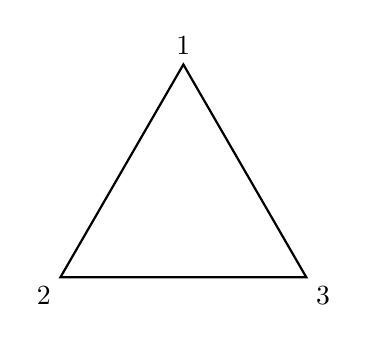
\begin{tikzpicture}[scale=1.2]
  % Vertices
  \coordinate (A) at (0,1.5);
  \coordinate (B) at (-1.3,-0.75);
  \coordinate (C) at (1.3,-0.75);
  \coordinate (O) at (0,0);

  % Triangle
  \draw[thick] (A) -- (B) -- (C) -- cycle;

  % Vertex labels
  \node[above] at (A) {1};
  \node[below left] at (B) {2};
  \node[below right] at (C) {3};

  % Center
  \coordinate (O) at (0,0);
\end{tikzpicture}
\end{center}

Let $f$ be a reflection through the vertical axis. So $f$ fixes point $1$ and switches $2$ and $3$.

Let $g$ be a rotation $120^\circ$ clockwise around the center point. So $g$ sends $1$ to $2$, $2$ to $3$, and $3$ to $1$.

There are four other symmetries of an equilateral triangle. What are they in terms of either an axis of reflection or an angle of rotation?

The composition of two symmetries is another symmetry, and this product is associative. There is an identity symmetry, and every symmetry has an inverse. Why? How would you justify these statements?

Hence, the symmetries of an equilateral triangle form a group under composition.
\end{define}

Match each symmetry on the left with an equivalent one from the right if possible. The notation $fg$ means $f \circ g$, so first rotate $120^\circ$, then reflect through the vertical axis.
\begin{enumerate}[label=\Alph*.]
  \item $g f$
  \item $g^{-1}$
  \item $g^2 f$
  \item $f$
  \item $f^2$
  \item None of the above
\end{enumerate}

Match the following.
\begin{enumerate}
  \item $f^{-1}$
  \item $g^3$
  \item $f g^2$
  \item $f g$
  \item $g^2$
\end{enumerate}


Fill in the product table below using the given labels for the symmetries. Let $e$ denote the identity symmetry. Enter $g^2$ as "gg" and $f g^2$ as "fgg".

\begin{tabular}{|c|c|c|c|c|c|c|}
\hline & $e$ & $f$ & $g$ & $g^2$ & $f g$ & $f g^2$ \\
\hline$e$ & & & & & & \\
\hline$f$ & & & & & \\
\hline$g$ & & & & & & \\
\hline$g^2$ & & & & & & \\
\hline$f g$ & & & & & & \\
\hline$f g^2$ & & & & & & \\
\hline
\end{tabular}


Definition: Let $(G, *)$ be a finite group with identity $e$. The order of an element $a \in G$, denoted $o(a)$, is the least positive integer $m$ such that $a^m=e$.

Let $(G, *)$ be the group of symmetries of an equilateral triangle under composition. What are the truth values of the following propositions?
\begin{enumerate}
  \item Every element in $(G, *)$ has order 2 or 3.
  \item $f g = g^{-1} f$ but $g \neq g^{-1}$.
  \item The order of $(G, *)$ is 6.
  \item The order of $g^2$ is 6.
  \item The order of $f$ is 2.
  \item $(f g)^2 \neq f^2 g^2$.
  \item For all elements $h \in G$, $h^6 = e$.
  \item The order of $g$ is 3.
  \item The order of every element in $(G, *)$ divides the order of the group.
  \item $g^2 (f g) = (f g) g^2$.
  \item $(G, *)$ is an abelian group.
\end{enumerate}




\newpage



Up to isomorphism, there is a unique group of order 5 . Let $G=\{a, b, c, d, e\}$ be a group with product *. Complete the product table for $(G, *)$ below.

\begin{center}
  \begin{tabular}{|l|c|c|c|c|c|}
  \hline$*$ & $e$ & $a$ & $b$ & $c$ & $d$ \\
  \hline$e$ & $e$ & $a$ & $b$ & $c$ & $d$ \\
  \hline$a$ & $a$ & $b$ & $d$ & $e$ & $c$ \\
  \hline$b$ & $b$ & $d$ & $c$ & $a$ & $e$ \\
  \hline$c$ & $c$ & $e$ & $a$ & $d$ & $b$ \\
  \hline$d$ & $d$ & $c$ & $e$ & $b$ & $a$ \\
  \hline
  \end{tabular}
\end{center}


The congruence classes modulo 5 are also a group of order 5 under addition. Show that ( $\setZ_5,+$ ) is isomorphic to $(G, *)$ in several different ways by completing the various bijections $\phi: \setZ_5 \rightarrow G$ below.

Match the elements of $\setZ_5$ on the left with their images in $G$. Remember that the bijection $\phi$ must preserve operations to be an isomorphism.


\begin{enumerate}
  \item Suppose $\phi$ maps $[1]$ to $a$.
  \begin{subanswer}
    \begin{itemize}
      \item $\phi([0]) \rightarrow e$
      \item $\phi([1]) \rightarrow a$
      \item $\phi([2]) \rightarrow a^2 = b$
      \item $\phi([3]) \rightarrow a^3 = d$
      \item $\phi([4]) \rightarrow a^4 = c$
    \end{itemize}
  \end{subanswer}
  \item Suppose $\phi$ maps $[1]$ to $b$.
  \begin{subanswer}
    \begin{itemize}
      \item $\phi([0]) \rightarrow e$
      \item $\phi([1]) \rightarrow b$
      \item $\phi([2]) \rightarrow b^2 = c$
      \item $\phi([3]) \rightarrow b^3 = a$
      \item $\phi([4]) \rightarrow b^4 = d$
    \end{itemize}
  \end{subanswer}
  
  \item Suppose $\phi$ maps $[1]$ to $c$.
  \begin{subanswer}
    \begin{itemize}
      \item $\phi([0]) \rightarrow e$
      \item $\phi([1]) \rightarrow c$
      \item $\phi([2]) \rightarrow c^2 = d$
      \item $\phi([3]) \rightarrow c^3 = b$
      \item $\phi([4]) \rightarrow c^4 = a$
    \end{itemize}
  \end{subanswer}
  \item Suppose $\phi$ maps $[1]$ to $d$.
  \begin{subanswer}
    \begin{itemize}
      \item $\phi([0]) \rightarrow e$ \hfill (identity: $d^0 = e$)
      \item $\phi([1]) \rightarrow d$ \hfill ($d^1 = d$)
      \item $\phi([2]) \rightarrow d^2 = a$ \hfill ($d^2 = a$ from the table)
      \item $\phi([3]) \rightarrow d^3 = c$ \hfill ($d^3 = c$ from the table)
      \item $\phi([4]) \rightarrow d^4 = b$ \hfill ($d^4 = b$ from the table)
    \end{itemize}
  \end{subanswer}
  \item Suppose $\phi$ maps $[2]$ to $a$.
  \begin{subanswer}
    \begin{itemize}
      \item $\phi([0]) \rightarrow e$ \hfill (identity: $a^0 = e$)
      \item $\phi([1]) \rightarrow d$ \hfill ($a^1 = a$, but $a = d^2$, so $d$ is the element after $e$ in the cycle)
      \item $\phi([2]) \rightarrow a$ \hfill (by assumption)
      \item $\phi([3]) \rightarrow c$ \hfill ($a^3 = c$ from the table)
      \item $\phi([4]) \rightarrow b$ \hfill ($a^4 = b$ from the table)
    \end{itemize}
  \end{subanswer}
  \item Suppose $\phi$ maps $[3]$ to $a$.
  \begin{subanswer}
    \begin{itemize}
      \item $\phi([0]) \rightarrow e$ \hfill (identity: $a^0 = e$)
      \item $\phi([1]) \rightarrow b$ \hfill ($a^1 = a$, $a^2 = b$)
      \item $\phi([2]) \rightarrow c$ \hfill ($a^3 = c$)
      \item $\phi([3]) \rightarrow a$ \hfill (by assumption)
      \item $\phi([4]) \rightarrow d$ \hfill ($a^4 = d$)
    \end{itemize}
  \end{subanswer}
  \item Suppose $\phi$ maps $[4]$ to $a$.
  \begin{subanswer}
    \begin{itemize}
      \item $\phi([0]) \rightarrow e$
      \item $\phi([1]) \rightarrow c$
      \item $\phi([2]) \rightarrow d$
      \item $\phi([3]) \rightarrow b$
      \item $\phi([4]) \rightarrow a$
    \end{itemize}
  \end{subanswer}
\end{enumerate}


\newpage














\section*{Overview}
The announcement asks you to practice the \textbf{Goldilocks principle} in mathematical writing: give \emph{just the right amount} of explanation — not too little and not too much. These notes explain what that means, give short course-related examples, a checklist you can use in class or on exams, and practical tips for practicing the skill.

\section{What the announcement means (short)}
\begin{itemize}
  \item \textbf{Too little:} You omit necessary steps or justification; the reader cannot follow or verify your reasoning.
  \item \textbf{Too much:} You repeat or restate obvious facts, or include irrelevant digressions that bury the main point.
  \item \textbf{Just right:} Provide the definitions you need, the logical steps that connect them, and a clear conclusion — compact, precise, and sufficient for the intended audience to verify the result.
\end{itemize}

\section{Why it matters beyond exams}
\begin{itemize}
  \item \emph{Homework \& assignments:} graders need enough to see you understood the idea — but not long-winded prose.
  \item \emph{Research / papers:} reviewers want clear, rigorous proofs and concise motivation.
  \item \emph{Coding / code review:} succinct comments and correct edge-case handling beat verbose, noisy comments.
  \item \emph{Presentations / teaching:} clarity and economy keep the audience engaged.
  \item \emph{Professional writing:} concise but sufficient detail (design docs, emails, bug reports) leads to faster, less-error-prone collaboration.
\end{itemize}

\section{Concrete course examples}
Below are short ``too little / too much / just right'' style model answers for typical course problems.

\subsection{Equivalence relation}
\begin{define}{Relation defined by divisibility}
Let \(R\) be a relation on \(\setZ\) defined by
\[
a \,R\, b \IFF 3 \mid (a-b).
\]
Show that \(R\) is an equivalence relation.
\end{define}

\paragraph{Just-right solution:}
\begin{subprove}
  \textbf{Reflexive.} For any \(a\in\setZ\), \(a-a=0\) and \(3\mid 0\); thus \(aRa\).
  \textbf{Symmetric.} If \(3\mid (a-b)\) then \(3\mid (b-a)\), so \(aRb\Rightarrow bRa\).
  \textbf{Transitive.} If \(3\mid (a-b)\) and \(3\mid (b-c)\), then \(3\mid (a-c)\); hence \(aRb\) and \(bRc\Rightarrow aRc\).
  Therefore \(R\) is reflexive, symmetric, and transitive, i.e., an equivalence relation.
\end{subprove}


\begin{define}{Function: bijectivity}
Let \(f:\setZ\to\setZ\) be defined by \(f(n)=n+1\). Prove \(f\) is bijective.
\end{define}

\paragraph{Just-right solution:}
\begin{subprove}
\textbf{Injective.} If \(f(a)=f(b)\) then \(a+1=b+1\), so \(a=b\).
\textbf{Surjective.} For arbitrary \(y\in\setZ\) choose \(x=y-1\). Then \(f(x)=x+1=y\).
Thus \(f\) is both injective and surjective, hence bijective.
\end{subprove}


\begin{define}{Partial order: subset relation}
Show \((\mathcal{P}(X),\subseteq)\) is a partially ordered set.
\end{define}

\paragraph{Just-right solution:}
\begin{subprove}
\textbf{Reflexive.} For any \(A\subseteq X\), \(A\subseteq A\).
\textbf{Antisymmetric.} If \(A\subseteq B\) and \(B\subseteq A\), then \(A=B\).
\textbf{Transitive.} If \(A\subseteq B\) and \(B\subseteq C\), then \(A\subseteq C\).
Hence \(\subseteq\) satisfies reflexivity, antisymmetry, and transitivity, so it is a partial order.
\end{subprove}

\section{A short checklist for ``Goldilocks'' answers}
Before submitting or handing in a solution, run this mental checklist:
\begin{enumerate}[label=\arabic*.]
  \item \textbf{State what you are proving} in one crisp sentence.
  \item \textbf{Give necessary definitions} (only those used in the argument).
  \item \textbf{Outline the plan} if the proof is longer than a couple of lines.
  \item \textbf{Do the steps:} each step should follow logically and be minimally justified.
  \item \textbf{Address edge cases} when relevant (e.g., empty set, domain restrictions).
  \item \textbf{Conclude clearly:} ``Hence ... is ...'' or similar.
  \item \textbf{Edit for redundancy:} remove repeated or obvious statements.
\end{enumerate}

\section{Practical tips to practice this skill}
\begin{itemize}
  \item After writing a solution, \emph{try removing one sentence}. If the argument still works, that sentence was probably redundant; if it breaks, put it back.
  \item Conversely, \emph{remove a justification line} — if the reader cannot fill the gap, restore the line.
  \item When reviewing classmates' solutions, mark places that are unclear (too little) or repetitive (too much).
  \item Time yourself: write a focused 5--7 line solution to a typical problem; this trains concise clarity.
\end{itemize}

\section*{One-line summary}
Think like a careful editor: include everything the reader needs to verify your claim, and nothing they don’t.

\medskip
\noindent If you'd like, I can:
\begin{itemize}
  \item Convert this to a handout-ready two-column format,
  \item Generate a short practice worksheet with three problems and model ``too little / too much / just right'' solutions, or
  \item Rewrite one of your past solutions into the three-style format so you can compare.
\end{itemize}


























\newpage

\section*{Propositions on Lattices and Chains}

The truth values for the following propositions are determined.

\begin{enumerate}
  \item Every finite lattice has a least element. \\
  \textbf{True}. By repeatedly taking the greatest lower bound (GLB) of pairs of elements in a finite lattice, one can find a single GLB for the entire set, which is the least element.

  \item The poset $(\{1,2,4,8,16\}, \mid)$ is a lattice. \\
  \textbf{True}. This poset is a chain (a totally ordered set), and every chain is a lattice. For any two elements $a,b$ where $a \mid b$, their LUB is $b$ and their GLB is $a$.

  \item If $A$ is a set, the poset $(\mathcal{P}(A), \subseteq)$ is a lattice. \\
  \textbf{True}. For any two subsets $X, Y \subseteq A$, their least upper bound (LUB) is their union ($X \cup Y$) and their greatest lower bound (GLB) is their intersection ($X \cap Y$).

  \item There exist an infinite lattice which has a least but not a greatest element. \\
  \textbf{True}. The set of positive integers with the divisibility relation, $(\setZ^{+}, \mid)$, is an infinite lattice. It has a least element (1) but no greatest element.

  \item If a poset is a lattice, then it is a chain. \\
  \textbf{False}. A lattice does not require every pair of elements to be comparable. For example, in the lattice $(\mathcal{P}(\{a, b\}), \subseteq)$, the elements $\{a\}$ and $\{b\}$ are incomparable.

  \item There exist an infinite lattice which has a greatest but not a least element. \\
  \textbf{True}. The set of negative integers with the divisibility relation, $(\setZ^{-}, \mid)$, is a lattice with a greatest element (-1) but no least element.

  \item Every finite lattice has a greatest element. \\
  \textbf{True}. This is the dual to proposition 1. By repeatedly taking the least upper bound (LUB) of elements, one can find a greatest element for the entire finite set.


  \item


  \item If a poset is a chain, then it is a lattice. \\
  \textbf{True}. In a chain, any two elements are comparable. If $a \preceq b$, their LUB is $b$ and their GLB is $a$. Since a LUB and GLB exist for every pair, every chain is a lattice.
  


  \item

  \item If a poset is a lattice, then its dual poset is also a lattice. \\
  \textbf{True}. The LUB in a poset becomes the GLB in its dual, and vice-versa. If LUBs and GLBs exist for all pairs in a poset, they are guaranteed to exist in its dual.

  \item Every nonempty finite subset of a lattice has a greatest lower bound. \\
  \textbf{True}. This property can be proven by induction on the size of the subset, repeatedly applying the pairwise GLB operation which is guaranteed to exist in a lattice.

  \item There exist an infinite lattice which has neither a least nor a greatest element. \\
  \textbf{True}. The set of integers with the standard order, $(\setZ, \leq)$, is a chain (and therefore a lattice) with no least and no greatest element.





  \item



  \item Every nonempty finite subset of a lattice has a least upper bound. \\
  \textbf{True}. This is the dual to proposition 12 and follows from the same inductive argument using the LUB operation.

  \item The poset $(\{1,2,3,4,5\}, \mid)$ is a lattice. \\
  \textbf{False}. A lattice requires a LUB for every pair to exist \emph{within the set}. The pair $\{2, 3\}$ has a least common multiple of 6, which is not in the set.
  
  \item The poset $(\setZ^{+}, \mid)$ is a lattice. \\
  \textbf{True}. For any two positive integers $a, b$, their GLB is their greatest common divisor ($\text{gcd}(a,b)$) and their LUB is their least common multiple ($\text{lcm}(a,b)$), both of which always exist.

  \item There exist an infinite lattice which has both a least and a greatest element. \\
  \textbf{True}. The power set of the natural numbers, $(\mathcal{P}(\mathbb{N}), \subseteq)$, is an infinite lattice with a least element ($\emptyset$) and a greatest element ($\mathbb{N}$). Another example is the set of real numbers in $[0,1]$ under $\leq$.

\end{enumerate}



\newpage


\noindent\textbf{1. Select all maximal elements.} \\
An element is maximal if no other element in the set is a multiple of it. \\
\textit{Correct options}: \textbf{F. 24} and \textbf{E. 45}.

\vspace{1em}
\noindent\textbf{2. Select all minimal elements.} \\
An element is minimal if it is not a multiple of any other element in the set. \\
\textit{Correct options}: \textbf{B. 5} and \textbf{C. 3}.

\vspace{1em}
\noindent\textbf{3. Select the greatest element if one exists.} \\
A greatest element must be a unique maximal element. As there are two maximal elements, no greatest element exists. \\
\textit{Correct option}: \textbf{G. None of the above}.

\vspace{1em}
\noindent\textbf{4. Select the least element if one exists.} \\
A least element must be a unique minimal element. As there are two minimal elements, no least element exists. \\
\textit{Correct option}: \textbf{G. None of the above}.

\vspace{1em}
\noindent\textbf{5. Select all upper bounds of $\{3,5\}$.} \\
An upper bound must be a multiple of both 3 and 5. The elements from the set that satisfy this are 15 and 45. \\
\textit{Correct options}: \textbf{F. 15} and \textbf{E. 45}.

\vspace{1em}
\noindent\textbf{6. Select the least upper bound of $\{3,5\}$ if one exists.} \\
The least upper bound is the minimum of the set of upper bounds $\{15, 45\}$. Since $15 \mid 45$, 15 is the minimum. \\
\textit{Correct option}: \textbf{C. 15}.

\vspace{1em}
\noindent\textbf{7. Select all lower bounds of $\{15,45\}$.} \\
A lower bound must divide both 15 and 45. The elements from the set that satisfy this are 3, 5, and 15. \\
\textit{Correct options}: \textbf{B. 3}, \textbf{E. 5}, and \textbf{C. 15}.

\vspace{1em}
\noindent\textbf{8. Select the greatest lower bound of $\{15,45\}$ if one exists.} \\
The greatest lower bound is the maximum of the set of lower bounds $\{3, 5, 15\}$. Since 3 and 5 both divide 15, 15 is the maximum. \\
\textit{Correct option}: \textbf{A. 15}.

\subsection*{Poset $(\{\{1\},\{2\},\{4\},\{1,2\},\{1,4\},\{2,4\},\{3,4\},\{1,3,4\},\{2,3,4\}\}, \subseteq)$}
For this poset, where the relation is "is a subset of", the following properties are identified:
\begin{itemize}
  \item \textbf{Minimal Elements} (no proper subsets in the collection): $\{\{1\}, \{2\}, \{4\}\}$
  \item \textbf{Maximal Elements} (not a proper subset of any other set): $\{\{1,2\}, \{1,3,4\}, \{2,3,4\}\}$
\end{itemize}

\noindent\textbf{1. Select all maximal elements.} \\
\textit{Correct options}: \textbf{H. \{1,2\}}, \textbf{I. \{1,3,4\}}, and \textbf{B. \{2,3,4\}}.

\vspace{1em}
\noindent\textbf{2. Select all minimal elements.} \\
\textit{Correct options}: \textbf{C. \{1\}}, \textbf{E. \{2\}}, and \textbf{B. \{4\}}.

\vspace{1em}
\noindent\textbf{3. Select the greatest element if one exists.} \\
There are three maximal elements, not a unique one. Therefore, no greatest element exists. \\
\textit{Correct option}: \textbf{J. None of the above}.

\vspace{1em}
\noindent\textbf{4. Select the least element if one exists.} \\
There are three minimal elements, not a unique one. Therefore, no least element exists. \\
\textit{Correct option}: \textbf{J. None of the above}.

\vspace{1em}
\noindent\textbf{5. Select all upper bounds of $\{\{2\},\{4\}\}$.} \\
An upper bound must contain both 2 and 4. The sets from the collection that satisfy this are $\{2,4\}$ and $\{2,3,4\}$. \\
\textit{Correct options}: \textbf{B. \{2,4\}} and \textbf{G. \{2,3,4\}}.

\vspace{1em}
\noindent\textbf{6. Select the least upper bound of $\{\{2\},\{4\}\}$ if one exists.} \\
The least upper bound is the minimum of the upper bounds $\{\{2,4\}, \{2,3,4\}\}$. Since $\{2,4\} \subseteq \{2,3,4\}$, $\{2,4\}$ is the minimum. \\
\textit{Correct option}: \textbf{D. \{2,4\}}.

\vspace{1em}
\noindent\textbf{7. Select all lower bounds of $\{\{1,3,4\},\{2,3,4\}\}$.} \\
A lower bound must be a subset of the intersection, which is $\{3,4\}$. The sets from the collection that are subsets of $\{3,4\}$ are $\{4\}$ and $\{3,4\}$. \\
\textit{Correct options}: \textbf{G. \{4\}} and \textbf{C. \{3,4\}}.

\vspace{1em}
\noindent\textbf{8. Select the greatest lower bound of $\{\{1,3,4\},\{2,3,4\}\}$ if one exists.} \\
The greatest lower bound is the maximum of the lower bounds $\{\{4\}, \{3,4\}\}$. Since $\{4\} \subseteq \{3,4\}$, $\{3,4\}$ is the maximum. \\
\textit{Correct option}: \textbf{D. \{3,4\}}.






\newpage

The truth values for the following propositions concerning partially ordered sets are determined. A pair of elements $a, b$ in a poset with relation $\preceq$ is considered \textbf{comparable} if either $a \preceq b$ or $b \preceq a$ holds true.

\begin{enumerate}
  \item If $a, b \in \mathbb{R}$, then $a$ and $b$ are comparable in the poset $(\mathbb{R}, \leq)$. \\
  \textbf{True}. For any two real numbers $a$ and $b$, it is always true that either $a \leq b$ or $b \leq a$. This is the definition of a total order.

  \item The elements 7 and 12 are comparable in the poset $(\setZ^{+}, \mid)$. \\
  \textbf{False}. Neither $7 \mid 12$ nor $12 \mid 7$ is true. Since neither element divides the other, they are incomparable.

  \item The elements 10 and 5 are comparable in the poset $(\setZ^{+}, \mid)$. \\
  \textbf{True}. While $10 \nmid 5$, it is true that $5 \mid 10$. Since one of the relations holds, they are comparable.

  \item The sets $\{1,2,3\}$ and $\{2,3,4\}$ are comparable in the poset $(\mathcal{P}(\setZ), \subseteq)$. \\
  \textbf{False}. Neither set is a subset of the other, so they are incomparable.

  \item The dual poset of $(\setZ, \mid)$ is $(\setZ, \nmid)$. \\
  \textbf{False}. The dual of the relation $a \mid b$ is $b \mid a$. The symbol $\nmid$ denotes the negation of the relation, not its dual.

  \item The sets $\{1,2\}$ and $\{1,2,3,4,5\}$ are comparable in the poset $(\mathcal{P}(\setZ), \subseteq)$. \\
  \textbf{True}. The set $\{1, 2\}$ is a subset of $\{1, 2, 3, 4, 5\}$, so they are comparable.

  \item The dual poset of $(\setZ, \leq)$ is $(\setZ,>)$. \\
  \textbf{False}. The dual of the relation $\leq$ is $\geq$. The relation $>$ is not a partial order because it is not reflexive.

  \item The sets $\{1,3,5\}$ and $\{2,4\}$ are comparable in the poset $(\mathcal{P}(\setZ), \subseteq)$. \\
  \textbf{False}. The sets are disjoint, so neither is a subset of the other. They are incomparable.

  \item The relation $\neq$ is a partial ordering of $\setZ$. \\
  \textbf{False}. A partial order must be reflexive, but $a \neq a$ is always false.

  \item The set $\emptyset$ is comparable to every element in the poset $(\mathcal{P}(\setZ), \subseteq)$. \\
  \textbf{True}. The empty set is a subset of every set, so $\emptyset \subseteq A$ is true for any set $A$, making them comparable.

  \item The elements 13 and 39 are comparable in the poset $(\setZ^{+}, \mid)$. \\
  \textbf{True}. Since $13 \mid 39$, the elements are comparable.

  \item The sets $\{3,5,7\}$ and $\{7\}$ are comparable in the poset $(\mathcal{P}(\setZ), \subseteq)$. \\
  \textbf{True}. The set $\{7\}$ is a subset of $\{3, 5, 7\}$, so they are comparable.

  \item The element 1 is comparable to all other elements in the poset $(\setZ^{+}, \mid)$. \\
  \textbf{True}. The number 1 divides every positive integer ($1 \mid k$ for all $k \in \setZ^{+}$), making it comparable to all other elements.

  \item The relation $=$ is both a partial order and an equivalence relation on $\mathbb{R}$. \\
  \textbf{True}. It is reflexive, antisymmetric, and transitive (a partial order). It is also reflexive, symmetric, and transitive (an equivalence relation).

  \item The set $\setZ$ is comparable to every element in the poset $(\mathcal{P}(\setZ), \subseteq)$. \\
  \textbf{True}. Every set $A \in \mathcal{P}(\setZ)$ is by definition a subset of $\setZ$, so $A \subseteq \setZ$ is always true.

  \item The dual poset of $(\mathcal{P}(\{0,1,2\}), \subseteq)$ is $(\mathcal{P}(\{0,1,2\}), \supseteq)$. \\
  \textbf{True}. The dual of the relation $A \subseteq B$ is $B \subseteq A$, which is equivalent to $A \supseteq B$.

  \item The elements 3 and 3 are comparable in the poset $(\setZ^{+}, \mid)$. \\
  \textbf{True}. Because the divisibility relation is reflexive, $3 \mid 3$ is true, which makes them comparable.

  \item The elements 6 and 9 are comparable in the poset $(\setZ^{+}, \mid)$. \\
  \textbf{False}. Neither $6 \mid 9$ nor $9 \mid 6$ is true. They are incomparable.

\end{enumerate}




\newpage


First, the six permutations on the set $\{1, 2, 3\}$ are explicitly defined for clarity. The permutation $c$, which was not explicitly defined in the problem description, is the transposition of 1 and 3.

\begin{itemize}
  \item $e = \begin{pmatrix} 1 & 2 & 3 \\ 1 & 2 & 3 \end{pmatrix}$ (identity)
  \item $a = \begin{pmatrix} 1 & 2 & 3 \\ 2 & 1 & 3 \end{pmatrix}$ (swaps 1 and 2)
  \item $b = \begin{pmatrix} 1 & 2 & 3 \\ 1 & 3 & 2 \end{pmatrix}$ (swaps 2 and 3)
  \item $c = \begin{pmatrix} 1 & 2 & 3 \\ 3 & 2 & 1 \end{pmatrix}$ (swaps 1 and 3)
  \item $d = \begin{pmatrix} 1 & 2 & 3 \\ 2 & 3 & 1 \end{pmatrix}$ (cycle $1 \to 2 \to 3 \to 1$)
  \item $f = \begin{pmatrix} 1 & 2 & 3 \\ 3 & 1 & 2 \end{pmatrix}$ (cycle $1 \to 3 \to 2 \to 1$)
\end{itemize}

\section*{Completed Product Table}
The completed composition table is presented below. The operation is defined as $(row) \circ (column)$.

\begin{center}
  \begin{tabular}{|c||c|c|c|c|c|c|}
    \hline
    \textbf{$\circ$} & \textbf{$e$} & \textbf{$a$} & \textbf{$b$} & \textbf{$c$} & \textbf{$d$} & \textbf{$f$} \\
    \hline\hline
    \textbf{$e$} & $e$ & $a$ & $b$ & $c$ & $d$ & $f$ \\
    \hline
    \textbf{$a$} & $a$ & $e$ & $d$ & $f$ & $b$ & $c$ \\
    \hline
    \textbf{$b$} & $b$ & $f$ & $e$ & $d$ & $c$ & $a$ \\
    \hline
    \textbf{$c$} & $c$ & $d$ & $f$ & $e$ & $a$ & $b$ \\
    \hline
    \textbf{$d$} & $d$ & $c$ & $a$ & $b$ & $f$ & $e$ \\
    \hline
    \textbf{$f$} & $f$ & $b$ & $c$ & $a$ & $e$ & $d$ \\
    \hline
  \end{tabular}
\end{center}

\section*{Analysis of the Table}

\subsection*{What patterns are seen in this table?}
\begin{itemize}
  \item \textbf{Identity Element}: The first row and first column are identical to the headers. This shows that $e$ is the identity element, as $e \circ x = x \circ e = x$ for any permutation $x$.
  \item \textbf{Not Commutative}: The table is not symmetric across its main diagonal. For example, $a \circ b = d$, but $b \circ a = f$. This confirms that the composition of permutations is not a commutative operation.
  \item \textbf{Closure}: Every entry in the table is one of the six original permutations. This means the set is closed under the operation of composition.
\end{itemize}

\subsection*{How many times does a permutation appear in a given row or column?}
Each permutation appears \textbf{exactly once} in each row and each column. This is known as the \textbf{Latin Square Property} and is a fundamental characteristic of a group's Cayley table.

\subsection*{Does every permutation have an inverse?}
\textbf{Yes}. For every permutation $x$, there exists a unique permutation $y$ (the inverse, $x^{-1}$) such that $x \circ y = e$ and $y \circ x = e$. These can be found by locating the identity element $e$ in each row and column.
\begin{itemize}
  \item The permutations $a, b,$ and $c$ are their own inverses: $a \circ a = e$, $b \circ b = e$, $c \circ c = e$.
  \item The permutations $d$ and $f$ are inverses of each other: $d \circ f = e$ and $f \circ d = e$.
  \item The identity $e$ is its own inverse: $e \circ e = e$.
\end{itemize}



\newpage

\section*{Cayley Tables and Properties for $\setZ_n$}

The completed Cayley tables for addition and multiplication in $\setZ_4$ and $\setZ_5$ are provided, followed by an analysis of their properties.

\subsection*{Cayley Tables for $\setZ_4$}
The set of congruence classes is $\setZ_4 = \{[0], [1], [2], [3]\}$.

\vspace{1em}
\noindent
\begin{minipage}{0.45\textwidth}
  \centering
  \textbf{Addition Modulo 4}
  \vspace{0.5em}
  \begin{tabular}{|c||c|c|c|c|}
    \hline
    $+$ & $[0]$ & $[1]$ & $[2]$ & $[3]$ \\
    \hline\hline
    $[0]$ & $[0]$ & $[1]$ & $[2]$ & $[3]$ \\
    \hline
    $[1]$ & $[1]$ & $[2]$ & $[3]$ & $[0]$ \\
    \hline
    $[2]$ & $[2]$ & $[3]$ & $[0]$ & $[1]$ \\
    \hline
    $[3]$ & $[3]$ & $[0]$ & $[1]$ & $[2]$ \\
    \hline
  \end{tabular}
\end{minipage}
\hfill
\begin{minipage}{0.45\textwidth}
  \centering
  \textbf{Multiplication Modulo 4}
  \vspace{0.5em}
  \begin{tabular}{|c||c|c|c|c|}
    \hline
    $\cdot$ & $[0]$ & $[1]$ & $[2]$ & $[3]$ \\
    \hline\hline
    $[0]$ & $[0]$ & $[0]$ & $[0]$ & $[0]$ \\
    \hline
    $[1]$ & $[0]$ & $[1]$ & $[2]$ & $[3]$ \\
    \hline
    $[2]$ & $[0]$ & $[2]$ & $[0]$ & $[2]$ \\
    \hline
    $[3]$ & $[0]$ & $[3]$ & $[2]$ & $[1]$ \\
    \hline
  \end{tabular}
\end{minipage}
\vspace{2em}


\subsection*{Cayley Tables for $\setZ_5$}
The set of congruence classes is $\setZ_5 = \{[0], [1], [2], [3], [4]\}$.

\vspace{1em}
\noindent
\begin{minipage}{0.45\textwidth}
  \centering
  \textbf{Addition Modulo 5}
  \vspace{0.5em}
  \begin{tabular}{|c||c|c|c|c|c|}
    \hline
    $+$ & $[0]$ & $[1]$ & $[2]$ & $[3]$ & $[4]$ \\
    \hline\hline
    $[0]$ & $[0]$ & $[1]$ & $[2]$ & $[3]$ & $[4]$ \\
    \hline
    $[1]$ & $[1]$ & $[2]$ & $[3]$ & $[4]$ & $[0]$ \\
    \hline
    $[2]$ & $[2]$ & $[3]$ & $[4]$ & $[0]$ & $[1]$ \\
    \hline
    $[3]$ & $[3]$ & $[4]$ & $[0]$ & $[1]$ & $[2]$ \\
    \hline
    $[4]$ & $[4]$ & $[0]$ & $[1]$ & $[2]$ & $[3]$ \\
    \hline
  \end{tabular}
\end{minipage}
\hfill
\begin{minipage}{0.45\textwidth}
  \centering
  \textbf{Multiplication Modulo 5}
  \vspace{0.5em}
  \begin{tabular}{|c||c|c|c|c|c|}
    \hline
    $\cdot$ & $[0]$ & $[1]$ & $[2]$ & $[3]$ & $[4]$ \\
    \hline\hline
    $[0]$ & $[0]$ & $[0]$ & $[0]$ & $[0]$ & $[0]$ \\
    \hline
    $[1]$ & $[0]$ & $[1]$ & $[2]$ & $[3]$ & $[4]$ \\
    \hline
    $[2]$ & $[0]$ & $[2]$ & $[4]$ & $[1]$ & $[3]$ \\
    \hline
    $[3]$ & $[0]$ & $[3]$ & $[1]$ & $[4]$ & $[2]$ \\
    \hline
    $[4]$ & $[0]$ & $[4]$ & $[3]$ & $[2]$ & $[1]$ \\
    \hline
  \end{tabular}
\end{minipage}
\vspace{2em}

\section*{Patterns and Properties}
The following observations are made from the tables.

\subsection*{General Patterns}
\begin{itemize}
  \item \textbf{Identity Elements}: For addition, $[0]$ is the identity element. For multiplication, $[1]$ is the identity element.
  \item \textbf{Symmetry}: All four tables are symmetric across the main diagonal.
\end{itemize}

\subsection*{Frequency of Classes in Rows/Columns}
\begin{itemize}
  \item \textbf{Addition}: For both $\setZ_4$ and $\setZ_5$, every congruence class appears \textbf{exactly once} in each row and each column. This property means the tables are \textbf{Latin squares}.
  \item \textbf{Multiplication}: The pattern is more complex.
  \begin{itemize}
    \item In $\setZ_4$, the rows/columns for $[1]$ and $[3]$ (classes corresponding to integers relatively prime to 4) contain each class exactly once. However, the row/column for $[2]$ contains only $[0]$ and $[2]$, each appearing twice. This is because 2 is a \textbf{zero divisor} ($[2] \cdot [2] = [0]$).
    \item In $\setZ_5$, since 5 is a \textbf{prime number}, all non-zero elements are relatively prime to 5. Consequently, in every row and column corresponding to a non-zero element, each congruence class appears \textbf{exactly once}.
  \end{itemize}
\end{itemize}

\subsection*{Commutativity and Associativity}
\begin{itemize}
  \item \textbf{Commutativity}: \textbf{Yes}, both operations are commutative. This is visually confirmed by the symmetry of the tables and holds because addition and multiplication of integers are commutative:
  \[ [a] + [b] = [a+b] = [b+a] = [b] + [a] \]
  \[ [a] \cdot [b] = [ab] = [ba] = [b] \cdot [a] \]
  \item \textbf{Associativity}: \textbf{Yes}, both operations are associative. This property is inherited from the associativity of operations in the integers ($\setZ$):
  \[ ([a] + [b]) + [c] = [(a+b)+c] = [a+(b+c)] = [a] + ([b] + [c]) \]
  \[ ([a] \cdot [b]) \cdot [c] = [(ab)c] = [a(bc)] = [a] \cdot ([b] \cdot [c]) \]
\end{itemize}

\newpage


The truth values for the following statements are determined. A statement is considered \textbf{true} if it holds for all functions and all subsets, while it is \textbf{false} if a single counterexample can be found. For the counterexamples provided, the function $f: \{1, 2, 3\} \to \{a, b, c\}$ defined by $f(1)=a$, $f(2)=b$, and $f(3)=a$ is used. This function is neither one-to-one nor onto.

\begin{enumerate}
  \item $f(A \cap B) \subseteq f(A) \cap f(B)$ \\
  \textbf{True}. If an element $y \in f(A \cap B)$, then $y = f(x)$ for some $x \in A \cap B$. Since $x \in A$ and $x \in B$, it follows that $f(x) \in f(A)$ and $f(x) \in f(B)$. Thus, $y \in f(A) \cap f(B)$.

  \item $f^{-1}(C \cup D) \subseteq f^{-1}(C) \cup f^{-1}(D)$ \\
  \textbf{True}. If $x \in f^{-1}(C \cup D)$, its image $f(x)$ is in $C \cup D$. This means $f(x) \in C$ or $f(x) \in D$, which implies $x \in f^{-1}(C)$ or $x \in f^{-1}(D)$.

  \item $f^{-1}(C) \cup f^{-1}(D) \subseteq f^{-1}(C \cup D)$ \\
  \textbf{True}. If $x \in f^{-1}(C) \cup f^{-1}(D)$, then $x \in f^{-1}(C)$ or $x \in f^{-1}(D)$. This means $f(x) \in C$ or $f(x) \in D$. Therefore, $f(x) \in C \cup D$, which means $x \in f^{-1}(C \cup D)$.

  \item $f(A) \cap f(B) \subseteq f(A \cap B)$ \\
  \textbf{False}. This can fail if the function is not one-to-one. Let $A=\{1\}$ and $B=\{3\}$. Then $f(A)=\{a\}$ and $f(B)=\{a\}$, so $f(A) \cap f(B) = \{a\}$. However, $A \cap B = \emptyset$, so $f(A \cap B) = \emptyset$. The statement $\{a\} \subseteq \emptyset$ is false.

  \item If $C \subseteq D$, then $f^{-1}(C) \subseteq f^{-1}(D)$. \\
  \textbf{True}. If $C \subseteq D$, then any element $x$ whose image $f(x) \in C$ also has its image in $D$. By definition, any $x \in f^{-1}(C)$ must also be in $f^{-1}(D)$.

  \item If $f^{-1}(C) \subseteq f^{-1}(D)$, then $C \subseteq D$. \\
  \textbf{False}. This can fail if the function is not onto. Let $C=\{c\}$ and $D=\{a\}$. The premise $f^{-1}(C) \subseteq f^{-1}(D)$ is true because $f^{-1}(C) = \emptyset$ and $f^{-1}(D)=\{1,3\}$. However, the conclusion $C \subseteq D$ is false.

  \item $f^{-1}(C) \cap f^{-1}(D) \subseteq f^{-1}(C \cap D)$ \\
  \textbf{True}. If $x \in f^{-1}(C) \cap f^{-1}(D)$, its image $f(x)$ is in both $C$ and $D$. Therefore, $f(x) \in C \cap D$, which means $x \in f^{-1}(C \cap D)$.

  \item $f\left(f^{-1}(C)\right) \subseteq C$ \\
  \textbf{True}. The set $f^{-1}(C)$ contains only elements that map into $C$. Therefore, the image of this set must be a subset of $C$.

  \item $f(A) \cup f(B) \subseteq f(A \cup B)$ \\
  \textbf{True}. If $y \in f(A) \cup f(B)$, then $y$ is the image of an element in $A$ or in $B$. In either case, it is the image of an element from $A \cup B$.

  \item $A \subseteq f^{-1}(f(A))$ \\
  \textbf{True}. Every $x \in A$ maps to an element $f(x) \in f(A)$. By the definition of inverse image, $x$ must therefore belong to the set of all elements that map into $f(A)$.

  \item $f(A \cup B) \subseteq f(A) \cup f(B)$ \\
  \textbf{True}. If $y \in f(A \cup B)$, it is the image of some $x \in A \cup B$. If $x \in A$, then $y \in f(A)$. If $x \in B$, then $y \in f(B)$. So, $y$ must be in $f(A) \cup f(B)$.

  \item $f^{-1}(C \cap D) \subseteq f^{-1}(C) \cap f^{-1}(D)$ \\
  \textbf{True}. If $x \in f^{-1}(C \cap D)$, its image $f(x) \in C \cap D$. This means $f(x) \in C$ and $f(x) \in D$. Therefore, $x$ is in both $f^{-1}(C)$ and $f^{-1}(D)$.

  \item $f^{-1}(f(A)) \subseteq A$ \\
  \textbf{False}. This can fail if the function is not one-to-one. Let $A=\{1\}$. Then $f(A)=\{a\}$. The inverse image $f^{-1}(\{a\})$ is $\{1, 3\}$. The statement $\{1, 3\} \subseteq \{1\}$ is false.

  \item If $f(A) \subseteq f(B)$, then $A \subseteq B$. \\
  \textbf{False}. This can fail if the function is not one-to-one. Let $A=\{1\}$ and $B=\{3\}$. Then $f(A)=\{a\}$ and $f(B)=\{a\}$. The premise $f(A) \subseteq f(B)$ is true, but the conclusion $A \subseteq B$ is false.

  \item $C \subseteq f\left(f^{-1}(C)\right)$ \\
  \textbf{False}. This can fail if the function is not onto. Let $C=\{c\}$. The inverse image $f^{-1}(\{c\})$ is $\emptyset$. The image $f(\emptyset)$ is also $\emptyset$. The statement $\{c\} \subseteq \emptyset$ is false.

  \item If $A \subseteq B$, then $f(A) \subseteq f(B)$. \\
  \textbf{True}. If $A$ is a subset of $B$, any element in $A$ is also in $B$. Therefore, the image of any element from $A$ must also be an image of an element from $B$.

\end{enumerate}



































% \newpage\handout[true]
% {\textsc{Math 2106-B: Foundations of Mathematical Proof}}{Fall 2025}
% {Homework 6: Groups and Subgroups}
% {\textit{Prof.} \href{https://ceheitsch.github.io/webpage/}{Dr. Christine Heitsch}}{Due Date: October 23, 2025}
% {Math 2106-B: HW6}
% {\large
  \noindent
  \textbf{Name:} \HandoutAuthor \smallskip \\

  \noindent
  \textbf{GTID:} 903743506 \smallskip \\

  \noindent
  %%% List anyone with whom you discussed the problems
  \textbf{Collaborators:} None. This material reflects independent preparation. \smallskip \\

  \noindent
  %%% List all resources used OTHER than the textbook, lecture notes, 
  %%% webwork problems, ICA questions, and previous homework assignments.
  \textbf{Outside resources:} This work was informed by MATH 2106 course materials 
  (ICAs: in-class activities and WebWork contents) from \HandoutInstitution\ (the course textbook is 
  Chartrand \parencite{chartrand_mathematical_2018}).   
  Outside references specifically include
  textbooks written by 
  Grimaldi \parencite{grimaldi_discrete_2004} (used in MATH 3012) and 
  Rosen \parencite{rosen_discrete_2019} (used in CS 2050). \smallskip \\

  \noindent
  \textbf{Notice}: The answers contain cross-references throughout this document as clickable hyperlinks in most PDF viewers. However, the Gradescope PDF view might not support clickable hyperlinks.
}
% \printbibliography[
  heading=bibintoc,   
  title={References}     % change “References” text if needed
]
% `heading=bibnumbered` if you prefer it numbered chapter (in \tableofcontents)
% `heading=bibintoc`    if you prefer it unnumbered but still in the ToC
% \newpage
% % \printbibliography[
  heading=bibintoc,   
  title={References}     % change “References” text if needed
]
% `heading=bibnumbered` if you prefer it numbered chapter (in \tableofcontents)
% `heading=bibintoc`    if you prefer it unnumbered but still in the ToC\newpage
% % The following table presents the standard logical equivalences from these sources together with 
the author's own (or the student, myself, Jaehoon Song) clarifications and labels where applicable.


\begin{table}[h!]
  \centering
  \renewcommand{\arraystretch}{1.2}
  \setlength{\tabcolsep}{8pt}
  \begin{tabular}{|p{5.0cm}|p{5.0cm}|p{5.2cm}|}
    \hline
    \rowcolor[HTML]{E0E0E0}
    \multicolumn{2}{|l|}{\textbf{Logical Equivalences}} & \textbf{Name} \\
    \hline
    $\,p \AND q \equiv q \AND p$ & $\,p \OR q \equiv q \OR p$ & Commutative Law \\
    \hline
    $\, (p \AND q) \AND r \equiv p \AND (q \AND r)$ & $\, (p \OR q) \OR r \equiv p \OR (q \OR r)$ & Associative Law \\
    \hline
    $\,p \AND (q \OR r) \equiv (p \AND q) \OR (p \AND r)$ & $\,p \OR (q \AND r) \equiv (p \OR q) \AND (p \OR r)$ & Distributive Law \\
    \hline
    $\,\overline{p \AND q} \equiv \sNOT{p} \OR \sNOT{q}$ & $\,\overline{p \OR q} \equiv \sNOT{p} \AND \sNOT{q}$ & DeMorgan's Law \\
    \hline
    \multicolumn{2}{|l|}{$\,\overline{\overline{p}} \equiv p$} & Double Negation law \\
    \hline
    $\,p \AND \boldsymbol{T} \equiv p$ & $\,p \OR \boldsymbol{F} \equiv p$ & Identity Law \\
    \hline
    $\,p \OR \boldsymbol{T} \equiv \boldsymbol{T}$ & $\,p \AND \boldsymbol{F} \equiv \boldsymbol{F}$ & Domination Law \\
    \hline
    $\,p \AND p \equiv p$ & $\,p \OR p \equiv p$ & Idempotent Law \\
    \hline
    \multicolumn{2}{|l|}{$\,p \THEN q \equiv \sNOT{p} \OR q$} & Implication Equivalence \\
    \hline
    \multicolumn{2}{|l|}{$\,\overline{p \THEN q} \equiv p \AND \sNOT{q}$} & Negation of Implication \\
    \hline
    \multicolumn{2}{|l|}{$\,p \THEN q \equiv \sNOT{q} \THEN \sNOT{p}$} & Contrapositive Equivalence \\
    \hline
    \multicolumn{2}{|l|}{$\,p \OR \sNOT{p} \equiv \boldsymbol{T}$} & Law of Tautology \\
    \hline
    \multicolumn{2}{|l|}{$\,p \AND \sNOT{p} \equiv \boldsymbol{F}$} & Law of Contradiction \\
    \hline
  \end{tabular}
\end{table}\newpage
% % 
The following definitions are presented from standard mathematical sources (\textbf{Sets}).
Clarifications and labels have been added where applicable.

\begin{define}{Basic Set Concepts}\phantomsection\label{def:basic-set-concepts} % \hyperref[def:basic-set-concepts]{YOUR_CONTEXT}
  \begin{enumerate}
    \item \textbf{Universal Set:} A universal set $\setUNIV$ is a
    set that contains all objects under consideration in a particular context or problem.
    \item \textbf{Empty Set:} The empty set, denoted $\setNULL$,
    is the unique set that contains no elements.
    \item \textbf{Subset:} Let $A$ and $B$ be sets. $A$ is a
    subset of $B$ ($A \subseteq B$) if (and only if)
    for all $x \in A$, $x \in B$.
    \item \textbf{Set Equality:} Let $A$ and $B$ be sets. The sets $A$ and $B$ are
    equal ($A = B$) if $A \subseteq B$ and $B \subseteq A$.
    \item \textbf{Power Set:} Let $A$ be a set. The power set of $A$, denoted $\sPOWER{A}$ or $2^A$,
    is the set of all subsets of $A$. That is, $\mathcal{P}(A) = \{S\in\setUNIV : S \subseteq A\}$.
  \end{enumerate}
\end{define}
The following definitions extend the understanding of set operations
and properties.


\begin{define}{Set Operations}\phantomsection\label{def:set-operations} % \hyperref[def:set-operations]{YOUR_CONTEXT}
  \begin{enumerate}
    \item \textbf{Complementary Set:} Let $A$ be a subset of the universal set $\setUNIV$.
    The complement of $A$, denoted $A^c$ or $\overline{A}$, is the set of all elements
    in $\setUNIV$ that are not in $A$. That is, $A^c = \{x \in \setUNIV : x \notin A\}$.
    \item \textbf{Union:} Let $A$ and $B$ be sets. The union of $A$ and $B$,
    denoted $A \cup B$, is the set of all elements that are in $A$, or in $B$, or in both.
    That is, $A \cup B = \{x : x \in A \lor x \in B\}$.
    \item \textbf{Intersection:} Let $A$ and $B$ be sets. The intersection of $A$ and $B$,
    denoted $A \cap B$, is the set of all elements that are in both $A$ and $B$.
    That is, $A \cap B = \{x : x \in A \land x \in B\}$.
    \item \textbf{Set Difference:} Let $A$, $B$ be subsets of a universal set $\setUNIV$.
    The set difference $A \sMINUS B$ is defined to be the set
    $\{ x \in \setUNIV \LDIV x \in A \text{ and } x \notin B\}$. \vspace*{10px}\\
    \textit{It is sometimes called the relative complement of $B$ in $A$,
    and denoted in the textbook as $A - B$.}
    \item \textbf{Cartesian Product:} Let $A$ and $B$ be sets. The Cartesian product of
    $A$ and $B$, denoted $A \sTIMES B$, is the set consisting of all ordered pairs:
    \[
    A \sTIMES B = \{(a, b) \LDIV a \in A, b \in B\}.
    \]
  \end{enumerate}
\end{define}


\newpage

The following claims are given in the reference as well. Let $A,B\in U$, a universal set.


\begin{claim}{Subset of Union: $A \subseteq \sOR{A}{B}$}\phantomsection\label{claim:subset-union} % \hyperref[claim:subset-union]{YOUR_CONTEXT}
  \begin{subprove}[bluecolor]
      Let $x\in U$, assume $x\in A$. Then the statement \inlinequote{$x\in A$ or $x\in B$} is true.
      Hence, by the definition, $\sOR{A}{B}=\{x\in U\LDIV x\in A$ or $x\in B\}$, $x\in \sOR{A}{B}$.
      Thus, $A \subseteq \sOR{A}{B}$.
  \end{subprove}
\end{claim}

\begin{claim}{Empty Subset: $\setNULL \subseteq A$}\phantomsection\label{claim:empty-subset} % \hyperref[claim:empty-subset]{YOUR_CONTEXT}
  \begin{subprove}[bluecolor]
      Let $x\in U$, assume $x\in \setNULL$. But there are no elements in $\setNULL$, so
      $x\in \setNULL$ is false. Since the premise is false, the implication if $x\in \setNULL$,
      then $x\in A$ is true. Thus, $\setNULL \subseteq A$ by definition of \hyperref[def:basic-set-concepts]{subsets}.
  \end{subprove}
\end{claim}

\begin{claim}{Subset as Equality: $\sOR{A}{B}=A$ if and only if $B\subseteq A$}\phantomsection\label{claim:subset-equality} % \hyperref[claim:subset-equality]{YOUR_CONTEXT}
  \begin{subprove}[bluecolor]
      Let $x\in U$, first, we assume $B\subseteq A$, we have already shown
      $A \subseteq \sOR{A}{B}$ by the claim, \hyperref[claim:subset-union]{Subset of Union}. 
      To show $\sOR{A}{B} \subseteq A$, assume $x\in \sOR{A}{B}$.
      By definition, $x\in A$ or $x\in B$. Considering $x\in B$ and assumption
      $B \subseteq A$, $x\in B$ implies $x\in A$. Thus, $\sOR{A}{B} \subseteq A$.
      Hence, if $B\subseteq A$, then $\sOR{A}{B} = A$. \vspace*{10px}\\
      Now, we assume $\sOR{A}{B}=A$. To show $B\subseteq A$, we now assume $x\in B$. Since $x\in B$, by definition
      of union, $x\in \sOR{A}{B} = A$. Therefore, $B\subseteq A$.
  \end{subprove}
\end{claim}


%%%%%%%%%%%%%%%%%%% 9/8/25

Let $\setUNIV$ be a set. 
\begin{claim}{ICA6}\phantomsection\label{claim:ica6} % \hyperref[claim:ica6]{YOUR_CONTEXT}
  For all $A,B\in\setUNIV$, $$A\sTIMES B =\setNULL\THEN \group{A=\setNULL\OR B=\setNULL}$$
  \begin{subprove}[bluecolor]
    Let $A,B\in\setUNIV$. We prove $A\sTIMES B=\setNULL$. Assume it is not the case that 
    $A=\setNULL$ or $B=\setNULL$. Thus, we have $A=\setNULL$ and $B=\setNULL$. 
    Since $A\ne\setNULL$ by assumption, there exists an element $a\in A$. Likewise, there 
    is some $b\in B$ since $B\ne\setNULL$. Thus, $\group{a,b}\in\sBUILD{(x,y)}{x\in A,y\in B}$ 
    by definition. But then, $A\sTIMES B\ne\setNULL$ by definition. Hence, the claim holds. 
  \end{subprove}
\end{claim}


\begin{define}{Relatively Prime Integers (Coprime)}\phantomsection\label{def:relatively-prime} % \hyperref[def:relatively-prime]{YOUR_CONTEXT}
  Let $x,y \in \mathbb{Z}$. The integers $x$ and $y$ are said to be
  \textbf{relatively prime} if and only if
  $\gcd(x,y) = 1$.
\end{define}
\newpage
% % The following definitions and axioms are presented from standard mathematical sources (\textbf{Number Theory}) together with the author's own (or the student, myself, Jaehoon Song) clarifications and labels where applicable.

\begin{define}{Integers}[def:integers][red]
  $\setZ$: the set of all integers
\end{define}

\begin{define}{Rational Numbers}[def:rational-numbers][red]
  $\setQ$: the set of all rational numbers
\end{define}

\begin{define}{Real Numbers}[def:real-numbers][red]
  $\setR$: the set of all real numbers
\end{define}

\begin{define}{Natural Numbers}[def:natural-numbers][red]
  $\setN$ or $\setZ_{>0}$: the set of all natural numbers which are the set of positive integers (not including $0$)
\end{define}

\begin{define}{Positive Real Numbers}[def:positive-real-numbers][red]
  $\setR_{>0}$: the set of all positive real numbers
\end{define}

\begin{define}{Non-negative Real Numbers}[def:non-negative-real-numbers][red]
  $\setR_{\geq 0}$: the set of all non-negative real numbers
\end{define}


\newpage

The following definitions and claims extend the understanding of integers.

Here are the ICA2 Definitions and Axioms as follows.

\begin{define}{Even Integer}[def:even-integer][red]
  An integer $n$ is \underbar{even} if there exists 
  (existential quantification logic $\exists$) an integer $k$ such that
  \[
  n = 2k.
  \]
\end{define}

\begin{define}{Odd Integer}[def:odd-integer][red]
  An integer $n$ is \underbar{odd} if 
  there exists some integer $k$ such that
  \[
  n = 2k + 1.
  \]
\end{define}

\begin{define}{Closure under Addition}[def:closure-addition][red]
  The sum of two integers is again an 
  integer. (Closure under addition)
\end{define}

\begin{define}{Closure under Multiplication}[def:closure-multiplication][red]
  The product of two integers is again 
  an integer. (Closure under multiplication)
\end{define}

\begin{define}{Odd if and only if Not Even}[def:odd-iff-not-even][red]
  An integer is odd if and only if it 
  is not even.
\end{define}

Here are the ICA3 Definitions and Axioms as follows.

\begin{define}{Universal Closure under Addition}[def:universal-closure-addition][red]
  The sum of two integers (Universal quantification for all, for every, for each) is again an integer. (Closure under addition)
\end{define}

\begin{define}{Universal Closure under Multiplication}[def:universal-closure-multiplication][red]
  The product of two integers (Universal quantification for all, for every, for each) is again an integer. (Closure under multiplication)
\end{define}

\begin{define}{Even Integer Square}[def:even-integer-square][red]
  An integer $n$ is even if and only if $n^2$ is even.
\end{define}

\newpage

The following claims are given in the reference as well.

\begin{define}{Sum of Even Integers}[claim:sum-even-integers][red]
  The sum of two even integers is again an even integer.
  \begin{subprove}[red]
    Let $x$ be an integer and $y$ be an integer ($\forall x,y \in \setZ$). 
    Suppose $x$ is even and $y$ is even. Then, by \nameref{def:even-integer}, there exists an integer 
    $k$ and an integer $j$ such that $x=2k$ and $y=2j$. Then, 
    $x+y=\left(2k\right)+\left(2j\right)=2\left(k+j\right)$. By \nameref{def:closure-addition}, since $k$ and 
    $j$ are integers, then so is $\left(k+j\right)$. Hence, by definition, $x+y$ is an 
    even integer.
  \end{subprove}
\end{define}

The following definitions extend the understanding of integers including divisibility.

\begin{define}{Divisibility}[def:divisibility][red]
  An integer $n$ divides an integer $m$, denoted $n \LDIV m$, if there 
  exists an integer $k$ such that $m=n k$. Otherwise, $n \nmid m$.
\end{define}

The following definitions extend the classification of real numbers into rational and irrational numbers.

\begin{define}{Rational Number}[def:rational-number][red]
  A real number $x$ is \underbar{rational} if there exist integers $a$ and $b$ with $b \neq 0$ such that $bx = a$.
  Otherwise, $x$ is \underbar{irrational}.

  \textbf{Note}: Compare the rational number definition with the even/odd axiom \inlinequote{odd iff not even} from \nameref{def:odd-iff-not-even}.
\end{define}

The following claims are given in the reference as well.

\begin{define}{Irrationality of $\sqrt{2}$}[claim:sqrt2-irrational][red]
  $\sqrt{2}$ is irrational.
  \begin{subprove}[red]
    Suppose $\sqrt{2}$ is rational. Then, by \nameref{def:rational-number}, there exists $a,b\in \setZ$ 
    with $b\ne 0$ such that $b\cdot\sqrt{2}=a$. We may further assume that any factors 
    common to $a$ and $b$ have already been removed.\\

    Then, squaring both sides, this yields $2\cdot b^2 = a^2$.
    Since products of integers are again integers by \nameref{def:closure-multiplication}, we have that $a^2,b^2\in \setZ$.
    Thus, by definition, $a^2$ is even. Therefore, by \nameref{def:even-integer-square}, $a$ is even. 
    Thus, there exists $c\in\setZ$ such that $a=2c$. Then
    $$
    2b^2=a^2={2c}^2=4c^2
    $$
    Then, $b^2=2c^2$. Then, as before, $b^2$ is even, so $b$ is even.
    However, $a$ and $b$ both being even contradicts the fact that any factors 
    common to $a$ and $b$ have already been removed.
  \end{subprove}
\end{define}






%%%%%%%%%%%%%%%%%%% New style (refactor model)
\begin{define}{Relatively Prime Integers (Coprime)}[def:relatively-prime][red]
  Let $x,y \in \mathbb{Z}$. The integers $x$ and $y$ are said to be
  \textbf{relatively prime} if and only if
  $\gcd(x,y) = 1$.
\end{define}\newpage
% %%%%%%%%%%%%%%%%%%%%%%%%%%%%%%%%%%%%%%%%%%%%%%%%%%%%%%%%%%%%%%%%%%%%%%%
% % References
% %%%%%%%%%%%%%%%%%%%%%%%%%%%%%%%%%%%%%%%%%%%%%%%%%%%%%%%%%%%%%%%%%%%%%%%
% \textbf{Remark}: The following definitions (or results) are already proved in class or on previous ICA, 
% Wbwk, Hmwk assignments, and contents of the textbook.



% \begin{define}{Groups}[def:group][red]
%   A \textbf{group} is a nonempty set \(G\) under the (binary) 
%   operation \(*: S \times S \to S\), denoted by \((G, *)\), such that
%   \begin{itemize}
%     \item \textbf{Closure:} For all \(a, b \in G\), \(a * b \in G\).
%     \item \textbf{Associativity:} For all \(a, b, c \in G\), \((a * b) * c = a * (b * c)\).
%     \item \textbf{Existence of Identity:} There exists an element \(e \in G\) 
%     such that for all \(a \in G\), \(e * a = a * e = a\).
%     \item \textbf{Existence of Inverse:} For each \(a \in G\), there exists an 
%     element \(a^{-1} \in G\) such that \(a * a^{-1} = a^{-1} * a = e\).
%   \end{itemize}
% \end{define}

% Let $(G, *)$ be a group with identity $e \in G$.
% \begin{define}{Subgroup}[def:subgroup][red]
%   A nonempty subset $H$ of $G$ is called a subgroup of $G$ if (and only if) ( $H, *$ ) is a group. (That is, $H$ itself is a group with respect to the product of $G$.)
% \end{define}
% \begin{define}{Subgroup Lemma}[lem:subgroup-lemma][red]
%   (To be proved on ICA15.) A subset $H \subseteq G$ is a subgroup of ( $G, *$ ) if (and only if) 
%   $H$ is nonempty, closed under the product of $G$, and contains inverses, i.e 
%   \begin{enumerate}
%     \item $H \neq \emptyset$,
%     \item for all $a, b \in H$, $a * b \in H$, and
%     \item for all $a \in H, a^{-1} \in H$.
%   \end{enumerate}
% \end{define}
% \begin{define}{Order of an Element}[def:order-of-an-element][red]
%   Let $G$ be a finite group. The \textbf{order} of an 
%   element $a \in G$, denoted $o(a)$, is the least positive 
%   integer $m$ such that $a^m=e$.
% \end{define}
% \begin{define}{Cyclic Subgroup}[def:cyclic-subgroup][red]
%   The cyclic subgroup generated by $a \in G$ is the 
%   set, $\left(a\right)=\left\{a^i \mid i \in \setZ\right\}$.
% \end{define}
% \begin{define}{Abelian Group}[def:abelian-group][red]
%   A group $(G, *)$ is called an \textbf{abelian group} (or \textbf{commutative group}) if for all $a, b \in G$, 
%   \[
%     a * b = b * a.
%   \]
% \end{define}
% %%%%%%%%%%%%%%%%%%%%%%%%%%%%%%%%%%%%%%%%%%%%%%%%%%%%%%%%%%%%%%%%%%%%%%%
% % Problems
% %%%%%%%%%%%%%%%%%%%%%%%%%%%%%%%%%%%%%%%%%%%%%%%%%%%%%%%%%%%%%%%%%%%%%%%
% \newpage
% \begin{enumerate} 
%   \item Consider the set $\setZ_2 \times \setZ_2$ under the product 
%   of coordinate-wise addition. Prove that this is an abelian group. 
%   \textit{This group, denoted $V_4$, is called the Klein 4-group\footnote{
%     The \textbf{Klein 4-group} is an example of an abelian group. 
%     It is the smallest non-cyclic abelian group with four elements.
%   }}.
%   \begin{define}{Abelian Group $\setZ_2$}[def:abelian-group-z2][red]
%     Let $\setZ_2=\{[0],[1]\}$ be \textbf{integers modulo $2$}, 
%     i.e., the \textbf{set of equivalence classes} of integers under 
%     the \textbf{equivalence relation} of congruence modulo $2$.
%     Then, $(\setZ_2, +)$ is an abelian group.
%     \begin{subprove}
%       The addition table for $\setZ_2$ is shown as follows.
%       \begin{center}
%         \renewcommand{\arraystretch}{1.2}% vertical padding
%         \begin{tabular}{|c||c|c|}
%         \hline
%         $+$ & $[0]$ & $[1]$ \\
%         \hline\hline
%         $[0]$ & $[0]$ & $[1]$ \\
%         \hline
%         $[1]$ & $[1]$ & $[0]$ \\
%         \hline
%         \end{tabular}
%       \end{center}
%       where $[0]$ is the identity element and every element is its own inverse.
%       Furthermore, the addition is clearly well-defined, closed, associative, and commutative by nature.
%       Therefore, by definition of \nameref{def:abelian-group}, $(\setZ_2, +)$ is an abelian group.
%     \end{subprove}
%   \end{define}
%   \begin{subprove}
%     Let $G = \setZ_2 \times \setZ_2 = \{([0],[0]), ([0],[1]), ([1],[0]), ([1],[1])\}$, 
%     where $\setZ_2 = \{[0], [1]\}$. 
%     The operation on $G$ is coordinate-wise addition, 
%     \begin{itemize}
%       \item \textbf{Closure:} 
%         Let $(a_1, b_1),(a_2, b_2)\in G$. 
%         The sum is defined as follows.
%         \[
%           (a_1, b_1) + (a_2, b_2) = (a_1 + a_2, b_1 + b_2)
%         \]
%         Since $a_1, a_2, b_1, b_2 \in \setZ_2$ and $(\setZ_2, +)$ is closed, 
%         $(a_1 + a_2) \in \setZ_2$ and $(b_1 + b_2) \in \setZ_2$.
%         Therefore, $G$ is closed under the operation.
%       \item \textbf{Associativity:}
%         Let $(a_1, b_1),(a_2, b_2),(a_3, b_3)\in G$. 
%         Then, by definition of the operation and associativity in $\setZ_2$,
%         \begin{align*}
%           ((a_1, b_1) + (a_2, b_2)) + (a_3, b_3) 
%           &= (a_1 + a_2, b_1 + b_2) + (a_3, b_3) = (a_1 + a_2 + a_3, b_1 + b_2 + b_3) \\
%           &= (a_1, b_1) + (a_2 + a_3, b_2 + b_3) = (a_1, b_1) + ((a_2, b_2) + (a_3, b_3)).
%         \end{align*}
%         Thus, $G$ is associative under the operation.
%       \item \textbf{Identity Element:}
%         Let $e = ([0],[0]) \in G$. Then for any $(a, b) \in G$:
%         \[
%           e + (a, b) = ([0],[0]) + (a, b) = ([0] + a, [0] + b) = (a, b),
%         \]
%         and
%         \[
%           (a, b) + e = (a, b) + ([0],[0]) = (a + [0], b + [0]) = (a, b).
%         \]
%         Thus, $e$ is the identity element in $G$.
%       \item \textbf{Inverses:}
%         Let $(a, b) \in G$. Since every element in $\setZ_2$ is its own inverse,
%         \[
%           (a, b) + (a, b)^{-1} = (a, b) + (a, b) = ([0],[0]) = e.
%         \]
%         Thus, every element in $G$ has an inverse, $(a, b)^{-1}=(a, b)$.
%       \item \textbf{Commutativity:}
%         Let $(a_1, b_1),(a_2, b_2)\in G$. 
%         Then, by definition of the operation and commutativity in $\setZ_2$,
%         \[
%           (a_1, b_1) + (a_2, b_2) = (a_1 + a_2, b_1 + b_2) = (a_2 + a_1, b_2 + b_1) = (a_2, b_2) + (a_1, b_1).
%         \]
%     \end{itemize}
%     Therefore, by definition of \nameref{def:abelian-group}, $G$ is an abelian group.
%   \end{subprove}








%   \newpage
%   \item The set $Z(G)=\{z \in G \mid z x=x z$ for all $x \in G\}$ is 
%   called the center of $G$. Prove that $Z(G)$ is a subgroup of $G$.
%   \begin{subprove}
%     Let $H = Z(G) = \{z \in G \mid z x = x z \text{ for all } x \in G\}$, i.e., $H\subseteq G$.
%     \begin{itemize}
%       \item \textbf{Nonemptyness (Identity):} Since $G$ is a group, it contains the identity element $e$. 
%       For any $x \in G$, we have $e x = x e = x$. 
%       Thus, $e \in H$, and hence $H$ is nonempty as it contains the identity element.
%       \item \textbf{Closure:} Let $a, b \in H$. 
%       Then, for any $x \in G$,
%       \[
%         (a b) x = a (b x) = a (x b) = (a x) b = (x a) b = x (a b).
%       \]
%       Thus, $a b \in H$, and hence $H$ is closed under the group operation.
%       \item \textbf{Inverses:} Let $a \in H$. 
%       Then, for any $x \in G$,
%       \[
%         a x = x a.
%       \]
%       By definition of \nameref{def:subgroup} and \nameref{def:group}, 
%       $a \in G$, so has an inverse $a^{-1} \in G$.
%       By the operation with $a^{-1}$,
%       \[
%         a^{-1} (a x) a^{-1} =x a^{-1} = a^{-1} x= a^{-1} (x a) a^{-1}.
%       \]
%       Thus, $a^{-1} \in H$, and hence every element in $H$ has an inverse in $H$.
%     \end{itemize}
%     Therefore, by the \nameref{lem:subgroup-lemma}, $Z(G)$ is a subgroup of $G$, \inlinequote{\textbf{center of $G$}}.
%   \end{subprove}
%   \item Let $a \in G$. The set $C(a)=\{g \in G \mid a g=g a\}$ is called 
%   the \textit{centralizer} of $a$. 
%   Prove that $C(a)$ is a subgroup of $G$ for all $a \in G$.
%   \begin{subprove}
%     Let $H = C(a) = \{g \in G \mid a g = g a\}$, i.e., $H\subseteq G$.
%     \begin{itemize}
%       \item \textbf{Nonemptyness (Identity):} Since $G$ is a group, it contains the identity element $e$. 
%       For any $a \in G$, we have $a e = e a = a$. 
%       Thus, $e \in H$, and hence $H$ is nonempty as it contains the identity element.
%       \item \textbf{Closure:} Let $g_1, g_2 \in H$. 
%       Then, 
%       \[
%         a (g_1 g_2) = (a g_1) g_2 = (g_1 a) g_2 = g_1 (a g_2) = g_1 (g_2 a) = (g_1 g_2) a.
%       \]
%       Thus, $g_1 g_2 \in H$, and hence $H$ is closed under the group operation.
%       \item \textbf{Inverses:} Let $g \in H$. 
%       Then, 
%       \[
%         a g = g a.
%       \]
%       By definition of \nameref{def:subgroup} and \nameref{def:group}, 
%       $g \in G$, so has an inverse $g^{-1} \in G$.
%       By the operation with $g^{-1}$,
%       \[
%         g^{-1} (a g) g^{-1} g^{-1} a=  a g^{-1} = g^{-1} (g a) g^{-1}.
%       \]
%       Thus, $g^{-1} \in H$, and hence every element in $H$ has an inverse in $H$.
%     \end{itemize}
%     Therefore, by the \nameref{lem:subgroup-lemma}, $C(a)$ is a subgroup of $G$, 
%     \inlinequote{\textbf{centralizer of $a$}}.
%   \end{subprove}







%   \newpage
%   \item Let $G$ be a finite group and $a \in G$. 
%   Prove there exists $n \in \setZ$ with $n>0$ such that $a^n=e$.
%   \textit{Observe that this means the order of an element in a finite group is well-defined}.
%   \begin{define}{Exponent Notation}[def:exponent-notation][red]
%     For $a \in G$, define $a^0=e$. 
%     For $i \in \setZ$ with $i \geq 1$, 
%     define $a^i=a * a^{i-1}$ and $a^{-i}=\left(a^{-1}\right)^i$. 
%     It follows that $a^n a^m=a^{n+m}$ and $\left(a^n\right)^m=a^{n m}$ for $n, m \in \setZ$.
%   \end{define}
%   \begin{subprove}
%     Let $G$ be a finite group and $a \in G$ for the sake of direct proof.
%     Consider the $\abs{G} + 1$ sequence of powers of $a$ as follows.
%     \[
%       a^0, a^1, a^2, a^3, \ldots, a^{\abs{G}}
%     \]
%     Since $G$ is finite, there are only finitely many distinct elements in $G$, i.e. $\abs{G}$.
%     By the pigeonhole principle, there must exist integers $m$ and $n$ with $0 \leq n < m \leq \abs{G}$ such that
%     \[
%       a^m = a^n.
%     \]
%     By \nameref{def:exponent-notation}, multiplying both sides by $a^{-m}$,
%     \[
%       a^{m-n} = e
%     \]
%     where $m-n \in \setZ$ by closure of integers.
%     Therefore, by direct proof, for any element $a$ in a finite group $G$, 
%     there exists a positive integer $n$ such that $a^n = e$.
%   \end{subprove}
%   \item Suppose that $a=a^{-1}$ for every $a \in G$. 
%   Prove that $G$ is abelian.
%   \begin{subprove}
%     Let $a, b \in G$ and suppose $a=a^{-1}$ for every $a \in G$ for the sake of direct proof.
%     Then, by definition of \nameref{def:group}, $ab \in G$ since it is closed under 
%     the group operation, so $ab=(ab)^{-1}$ by the assumption. Thus,
%     \[
%       ab = (a b)^{-1} = b^{-1} a^{-1} = b a
%     \]
%     by \nameref{def:exponent-notation}.
%     Since $a$ and $b$ were arbitrary elements of $G$, 
%     it follows that for all $a, b \in G$, $a b = b a$.
%     Thus, by definition of \nameref{def:abelian-group}, $G$ is abelian.
%   \end{subprove}










%   \newpage
%   \item Let $H$ be a subgroup of $G$. Define a relation $R_H$ on $G$ 
%   where $(a, b) \in R$ if $a b^{-1} \in H$ for all $a, b \in G$. 
%   Prove that $R_H$ is an equivalence relation on $G$.
%   \begin{define}{Equivalence Relation}[def:equivalence-relation][red]
%     Let $S$ be a nonempty set. A binary relation $R$ on $S$ (i.e., a subset $R \subseteq S \times S$) is designated an \emph{equivalence relation} if and only if it satisfies the following three axioms:
%     \begin{itemize}
%       \item \textbf{Reflexivity:} Every element in $S$ is related to itself.
%         $$ \forall x \in S, \; (x,x) \in R $$
%       \item \textbf{Symmetry:} If an element $x$ is related to an element $y$, then $y$ is also related to $x$.
%         $$ \forall x,y \in S, \; (x,y) \in R \THEN (y,x) \in R $$
%       \item \textbf{Transitivity:} If an element $x$ is related to $y$, and $y$ is related to $z$, then $x$ is related to $z$.
%         $$ \forall x,y,z \in S, \; \left( (x,y) \in R \land (y,z) \in R \right) \THEN (x,z) \in R $$
%     \end{itemize}
%     where the \textbf{equivalence class} of $a$ with respect to $R$, denoted $[a]_R$, is defined 
%     as follows for any element $x \in S$. 
%     $$
%     [a]_R = \{x \in S \mid (a,x) \in R \}
%     $$
%   \end{define}
%   \begin{subprove}
%     Let $H$ be a subgroup of $G$ and let $R_H$ be the relation on $G$ defined by 
%     $(a, b) \in R_H$ if and only if $a b^{-1} \in H$ for all $a, b \in G$.
%     \begin{itemize}
%       \item \textbf{Reflexivity:} 
%         Let $a \in G$. 
%         Then, 
%         \[
%           a a^{-1} = e \in H
%         \]
%         since $H$ is a subgroup of $G$ and contains the identity element.
%         Thus, $(a, a) \in R_H$, and hence $R_H$ is reflexive.
%       \item \textbf{Symmetry:} 
%         Let $(a, b) \in R_H$. 
%         Then, 
%         \[
%           a b^{-1} \in H.
%         \]
%         By definition of subgroup, the inverse of any element in $H$ is also in $H$, so
%         \[
%           (a b^{-1})^{-1} = b a^{-1} \in H.
%         \]
%         Thus, $(b, a) \in R_H$, and hence $R_H$ is symmetric.
%       \item \textbf{Transitivity:} 
%         Let $(a, b) \in R_H$ and $(b, c) \in R_H$. 
%         Then,
%         \[
%           a b^{-1} \in H
%         \]
%         and
%         \[
%           b c^{-1} \in H.
%         \]
%         Since $H$ is closed under the group operation,
%         \[
%           (a b^{-1})(b c^{-1}) = a c^{-1} \in H.
%         \]
%         Thus, $(a, c) \in R_H$, and hence $R_H$ is transitive.
%     \end{itemize}
%     Therefore, by definition of \nameref{def:equivalence-relation}, $R_H$ is an equivalence relation on $G$.
%   \end{subprove}







%   \newpage
%   \item Define a relation $R$ on $G$ where $(a, b) \in R$ if 
%   there exists $x \in G$ such that $b=x^{-1} a x$. 
%   Prove that $R$ is an equivalence relation on $G$.
%   \begin{subprove}
%     Let $R$ be the relation on $G$ defined by 
%     $(a, b) \in R$ if and only if there exists $x \in G$ such that $b = x^{-1} a x$.
%     \begin{itemize}
%       \item \textbf{Reflexivity:} 
%         Let $a \in G$. 
%         Then, by taking $x = e$, the identity element in $G$,
%         \[
%           b = e^{-1} a e = a.
%         \]
%         Thus, $(a, a) \in R$, and hence $R$ is reflexive.
%       \item \textbf{Symmetry:} 
%         Let $(a, b) \in R$. 
%         Then, there exists $x \in G$ such that
%         \[
%           b = x^{-1} a x.
%         \]
%         Moreover,
%         \[
%           a = (x x^{-1}) a (x x^{-1}) = x b x^{-1} = (x^{-1})^{-1} b x^{-1}.
%         \]
%         where $x^{-1} \in G$ by definition of \nameref{def:group}. 
%         Thus, $(b, a) \in R$, and hence $R$ is symmetric.
%       \item \textbf{Transitivity:} 
%         Let $(a, b) \in R$ and $(b, c) \in R$. 
%         Then, there exist $x, y \in G$ such that
%         \[
%           b = x^{-1} a x
%         \]
%         and
%         \[
%           c = y^{-1} b y.
%         \]
%         Then, 
%         \[
%           c = y^{-1} (x^{-1} a x) y = (x y)^{-1} a (x y).
%         \]
%         where $xy\in G$ since groups are closed under the product of $G$.
%         Thus, $(a, c) \in R$, and hence $R$ is transitive.
%     \end{itemize}
%     Therefore, by definition of \nameref{def:equivalence-relation}, $R$ is an equivalence relation on $G$.
%   \end{subprove}











%   \newpage
%   \item Complete but do not hand in.
%   Let $G=S_3$, the symmetric group of degree 3, from ICA13. 
%   It is also $D_6$, the dihedral group of order 6, i.e. 
%   symmetries of the equilateral triangle (from the warm-up and webwork).
%   \begin{define}{Symmetric Group}[def:symmetric-group][red]
%     The symmetric group of degree $n$, denoted $S_n$, is the group of all permutations (bijective maps) of the set $\{1,\dots,n\}$ with composition as the group operation:
%     \[
%       S_n=\{\sigma:\{1,\dots,n\}\to\{1,\dots,n\}\mid \sigma\ \text{is a bijection}\}
%     \]
%     Note that $\abs{S_n}=n!$.
%   \end{define}
%   \begin{define}{Dihedral Group}[def:dihedral-group][red]
%     The dihedral group of order $2n$ (for $n \geq 3$), denoted $D_{2n}$, is the group of symmetries of a 
%     regular $n$-gon. It has the presentation
%     \[
%     D_{2n}=\langle r,s \mid r^n=e,\; s^2=e,\; srs=r^{-1}\rangle
%     \]
%     where $r$ is a rotation of order $n$ and $s$ a reflection of order $2$. 
%     Thus, $\lvert D_{2n}\rvert=2n$. 
%     % Intuitive picture and quick reference for D_6 (the equilateral triangle)
%     \begin{center}
%       % If your document does not yet load tikz, add \usepackage{tikz} in the preamble.
%       \begin{tikzpicture}[scale=2, every node/.style={font=\small}]
%       % triangle vertices
%       \coordinate (A) at (90:1);   % vertex 1 (top)
%       \coordinate (B) at (210:1);  % vertex 2 (left)
%       \coordinate (C) at (330:1);  % vertex 3 (right)
%       % draw triangle
%       \draw[thick] (A) -- (B) -- (C) -- cycle;
%       % labels
%       \node[above] at (A) {1};
%       \node[left]  at (B) {2};
%       \node[right] at (C) {3};

%       % center
%       \coordinate (O) at (0,0);
%       \fill (O) circle (0.6pt);

%       % dashed vertical axis (mirror axis for s)
%       \draw[dashed] (0,1.2) -- (0,-1.2) node[above right] {axis of $s$};

%       % small counter-clockwise rotation arrow for r
%       \draw[->, >=stealth, thick] (0.35,0) arc (0:120:0.35) node[pos=0.5, above] {$r$};
%       % double-headed curved arrow for s crossing the dashed axis (swap 2 <-> 3), small size
%       \draw[<->, >=stealth, thick] (210:0.5) arc (210:330:0.5) node[pos=0.5, above right] {$s$};      
%       \end{tikzpicture}
%     \end{center}
%   \end{define}



  
%   \newpage
%   \begin{enumerate}
%     \item Find the order of every $a \in G$.
%     \begin{subanswer}
%       Let $G = S_3 = \{e, x, x^2, a, xa, x^2a\}$. The order of an element $g$, $o(g)$, is the smallest positive integer $m$ such that $g^m = e$.
%       \begin{itemize}
%         \item \textbf{Order 1:} $o(e) = 1$.
%         \item \textbf{Order 2:} The elements of order 2 are the reflections.
%         \begin{itemize}
%           \item $o(a) = 2$, since $a^2 = e$.
%           \item $o(xa) = 2$, since $(xa)^2 = (xa)(xa) = x(ax)a = x(x^2a)a = x^3a^2 = (e)(e) = e$.
%           \item $o(x^2a) = 2$, since $(x^2a)^2 = (x^2a)(x^2a) = x^2(ax^2)a = x^2(xa)a = x^3a^2 = (e)(e) = e$.
%         \end{itemize}
%         \item \textbf{Order 3:} The elements of order 3 are the non-identity rotations.
%         \begin{itemize}
%           \item $o(x) = 3$, since $x^3 = e$.
%           \item $o(x^2) = 3$, since $(x^2)^3 = x^6 = (x^3)^2 = e^2 = e$.
%         \end{itemize}
%       \end{itemize}
%     \end{subanswer}

%     \item Find all subgroups $H \subseteq G$. \textit{Hint: there are 6 for $S_3$}.
%     \begin{subanswer}
%       By Lagrange's Theorem, subgroups must have an order dividing $\abs{G}=6$. The possible orders are 1, 2, 3, and 6.
%       \begin{itemize}
%         \item \textbf{Order 1 (Trivial):} $H_1 = \{e\}$
%         \item \textbf{Order 2 (Cyclic):} Generated by the three elements of order 2.
%         \begin{itemize}
%           \item $H_2 = \langle a \rangle = \{e, a\}$
%           \item $H_3 = \langle xa \rangle = \{e, xa\}$
%           \item $H_4 = \langle x^2a \rangle = \{e, x^2a\}$
%         \end{itemize}
%         \item \textbf{Order 3 (Cyclic):} Generated by the two elements of order 3.
%         \begin{itemize}
%           \item $H_5 = \langle x \rangle = \langle x^2 \rangle = \{e, x, x^2\}$
%         \end{itemize}
%         \item \textbf{Order 6 (The group itself):} $H_6 = G = \{e, x, x^2, a, xa, x^2a\}$
%       \end{itemize}
%     \end{subanswer}

%     \item Identify $Z(G)$. Identify $\langle a \rangle$ and $C(a)$ for each $a \in G$.
%     \begin{subanswer}
%       \begin{itemize}
%         \item \textbf{Center $Z(G)$:} The set of elements that commute with all 
%         elements in $G$. Since $xa = ax^2 \neq ax$, $x$ does not commute with 
%         $a$. Since the group is non-abelian, the center is a proper subgroup. 
%         A quick check shows that only the identity commutes with all 6 elements.
%           \[ Z(G) = \{e\} \]
%         \item \textbf{Cyclic Subgroups $\langle a \rangle$:}
%           \begin{itemize}
%             \item $\langle e \rangle = \{e\}$
%             \item $\langle x \rangle = \langle x^2 \rangle = \{e, x, x^2\}$
%             \item $\langle a \rangle = \{e, a\}$
%             \item $\langle xa \rangle = \{e, xa\}$
%             \item $\langle x^2a \rangle = \{e, x^2a\}$
%           \end{itemize}
%         \item \textbf{Centralizers $C(a) = \{g \in G \mid ga = ag\}$:}
%           \begin{itemize}
%             \item $C(e) = G$
%             \item $C(x) = \{g \mid gx = xg\}$. The elements that commute with $x$ are $e, x, x^2$.
%               \[ C(x) = \{e, x, x^2\} \]
%             \item $C(x^2) = \{g \mid gx^2 = x^2g\}$. Since $g$ commutes with $x^2$ iff it commutes with $x$,
%               \[ C(x^2) = \{e, x, x^2\} \]
%             \item $C(a) = \{g \mid ga = ag\}$. Only $e$ and $a$ commute with $a$.
%               \[ C(a) = \{e, a\} \]
%             \item $C(xa) = \{g \mid g(xa) = (xa)g\}$. Only $e$ and $xa$ commute with $xa$.
%               \[ C(xa) = \{e, xa\} \]
%             \item $C(x^2a) = \{g \mid g(x^2a) = (x^2a)g\}$. Only $e$ and $x^2a$ commute with $x^2a$.
%               \[ C(x^2a) = \{e, x^2a\} \]
%           \end{itemize}
%       \end{itemize}
%     \end{subanswer}

%     \item For each subgroup $H$, find the equivalence classes under the relation $R_H$ in problem 6.
%     \begin{subanswer}
%       The relation is $(a, b) \in R_H$ if $ab^{-1} \in H$. The equivalence classes $[a] = \{b \mid ab^{-1} \in H\}$ are the \textbf{right cosets $Ha = \{ha \mid h \in H\}$}.
%       \begin{itemize}
%         \item \textbf{$H_1 = \{e\}$:} The cosets are the elements themselves.
%           \begin{itemize}
%             \item $[e] = \{e\}$, $[x] = \{x\}$, $[x^2] = \{x^2\}$, $[a] = \{a\}$, $[xa] = \{xa\}$, $[x^2a] = \{x^2a\}$
%           \end{itemize}
%         \item \textbf{$H_2 = \{e, a\}$:}
%           \begin{itemize}
%             \item $H_2e = \{e \cdot e, a \cdot e\} = \{e, a\}$
%             \item $H_2x = \{e \cdot x, a \cdot x\} = \{x, ax\} = \{x, x^2a\}$
%             \item $H_2x^2 = \{e \cdot x^2, a \cdot x^2\} = \{x^2, ax^2\} = \{x^2, xa\}$
%           \end{itemize}
%         \item \textbf{$H_3 = \{e, xa\}$:}
%           \begin{itemize}
%             \item $H_3e = \{e, xa\}$
%             \item $H_3x = \{x, (xa)x\} = \{x, a\}$
%             \item $H_3x^2 = \{x^2, (xa)x^2\} = \{x^2, x^2a\}$
%           \end{itemize}
%         \item \textbf{$H_4 = \{e, x^2a\}$:}
%           \begin{itemize}
%             \item $H_4e = \{e, x^2a\}$
%             \item $H_4x = \{x, (x^2a)x\} = \{x, xa\}$
%             \item $H_4x^2 = \{x^2, (x^2a)x^2\} = \{x^2, a\}$
%           \end{itemize}
%         \item \textbf{$H_5 = \{e, x, x^2\}$:} (This is a normal subgroup)
%           \begin{itemize}
%             \item $H_5e = \{e \cdot e, x \cdot e, x^2 \cdot e\} = \{e, x, x^2\}$
%             \item $H_5a = \{e \cdot a, x \cdot a, x^2 \cdot a\} = \{a, xa, x^2a\}$
%           \end{itemize}
%         \item \textbf{$H_6 = G$:}
%           \begin{itemize}
%             \item $H_6e = G = \{e, x, x^2, a, xa, x^2a\}$
%           \end{itemize}
%       \end{itemize}
%     \end{subanswer}

%     \item For each $a \in G$, find its equivalence class under the relation $R$ from problem 7.
%     \begin{subanswer}
%       The relation is $(a, b) \in R$ if $b = g^{-1} a g$ for some $g \in G$. These are the \textbf{conjugacy classes}.
%       \begin{itemize}
%         \item \textbf{$[e]$:} The class of the identity is always just the identity.
%           \[ [e] = \{g^{-1}eg \mid g \in G\} = \{e\} \]
%         \item \textbf{$[x]$:} The class of rotations.
%           \begin{itemize}
%             \item $e^{-1}xe = x$
%             \item $x^{-1}xx = x$
%             \item $(x^2)^{-1}xx^2 = x(x)x^2 = x^4 = x$
%             \item $a^{-1}xa = axa = a(ax^2) = x^2$
%             \item $(xa)^{-1}x(xa) = (xa)x(xa) = (xa)(x^2a) = x(a x^2 a) = x(a(xa)) = x(x) = x^2$
%             \item $(x^2a)^{-1}x(x^2a) = (x^2a)x(x^2a) = (xa)(x^2a) = x(ax^2a) = x(a(xa)) = x(x) = x^2$
%           \end{itemize}
%           \[ [x] = \{x, x^2\} \]
%         \item \textbf{$[x^2]$:} Since $x^2 \in [x]$, $[x^2] = [x] = \{x, x^2\}$.
%         \item \textbf{$[a]$:} The class of reflections.
%           \begin{itemize}
%             \item $e^{-1}ae = a$
%             \item $x^{-1}ax = x^2(ax) = x^2(x^2a) = x^4a = xa$
%             \item $(x^2)^{-1}ax^2 = x(ax^2) = x(xa) = x^2a$
%           \end{itemize}
%           (All other conjugates will also land in this set).
%           \[ [a] = \{a, xa, x^2a\} \]
%         \item \textbf{$[xa]$:} Since $xa \in [a]$, $[xa] = [a] = \{a, xa, x^2a\}$.
%         \item \textbf{$[x^2a]$:} Since $x^2a \in [a]$, $[x^2a] = [a] = \{a, xa, x^2a\}$.
%       \end{itemize}
%       The distinct conjugacy classes are: $\{e\}$, $\{x, x^2\}$, and $\{a, xa, x^2a\}$.
%     \end{subanswer}
%   \end{enumerate}
  

%   \newpage
%   \item Repeat problem 8 where $G=D_8$, the dihedral group of order 8. 
%   \textit{Hint: there are 10 subgroups}.
%   \begin{enumerate}
%     \item Find the order of every $a \in G$.
%     \begin{subanswer}
%       The elements of $D_8$ are: $e$, $r$, $r^2$, $r^3$, $s$, $sr$, $sr^2$, $sr^3$.
%       \begin{itemize}
%         \item $o(e) = 1$
%         \item $o(r) = 4$
%         \item $o(r^2) = 2$
%         \item $o(r^3) = 4$
%         \item $o(s) = 2$
%         \item $o(sr) = 2$
%         \item $o(sr^2) = 2$
%         \item $o(sr^3) = 2$
%       \end{itemize}
%     \end{subanswer}
%     \item Find all subgroups $H \subseteq G$. \textit{Hint: there are 6 for $S_3$}.
%     \begin{subanswer}
%       The subgroups of $D_8$ are:
%       \begin{itemize}
%         \item $H_1 = \{e\}$
%         \item $H_2 = \{e, r^2\}$
%         \item $H_3 = \{e, r, r^2, r^3\}$
%         \item $H_4 = \{e, s\}$
%         \item $H_5 = \{e, sr^2\}$
%         \item $H_6 = D_8$
%       \end{itemize}
%     \end{subanswer}
%     \item Identify $Z(G)$. Identify $(a)$ and $C(a)$ for each $a \in G$.
%     \begin{subanswer}
%       The center $Z(G)$ consists of all elements that commute with every element of $G$. In $D_8$, we have:
%       \begin{itemize}
%         \item $Z(D_8) = \{e, r^2\}$
%       \end{itemize}
%       The centralizer $C(a)$ for each $a \in G$ is:
%       \begin{itemize}
%         \item $C(e) = D_8$
%         \item $C(r) = \{e, r, r^2, r^3\}$
%         \item $C(r^2) = D_8$
%         \item $C(r^3) = \{e, r, r^2, r^3\}$
%         \item $C(s) = \{e, s\}$
%         \item $C(sr) = \{e, sr\}$
%         \item $C(sr^2) = \{e, sr^2\}$
%         \item $C(sr^3) = \{e, sr^3\}$
%       \end{itemize}
%     \end{subanswer}
%     \item For each subgroup $H$, find the equivalence classes under the relation $R_H$ in problem 6.
%     \begin{subanswer}
%       The equivalence classes under the relation $R_H$ are:
%       \begin{itemize}
%         \item For $H_1 = \{e\}$: Each element forms its own class.
%         \item For $H_2 = \{e, r^2\}$: Classes are $\{e, r^2\}$, $\{r, r^3\}$, $\{s, sr^2\}$, $\{sr, sr^3\}$.
%         \item For $H_3 = \{e, r, r^2, r^3\}$: Classes are $\{e, r, r^2, r^3\}$ and $\{s, sr, sr^2, sr^3\}$.
%         \item For $H_4 = \{e, s\}$: Classes are $\{e, s\}$, $\{r, sr\}$, $\{r^2, sr^2\}$, $\{r^3, sr^3\}$.
%         \item For $H_5 = \{e, sr^2\}$: Classes are $\{e, sr^2\}$, $\{r, sr^3\}$, $\{r^2, s\}$, $\{r^3, sr\}$.
%         \item For $H_6 = D_8$: The entire group is one class.
%       \end{itemize}
%     \end{subanswer}
%     \item For each $a \in G$, find its equivalence class under the relation $R$ from problem 7.
%     \begin{subanswer}
%       The conjugacy classes in $D_8$ are:
%       \begin{itemize}
%         \item $[e] = \{e\}$
%         \item $[r] = \{r, r^3\}$
%         \item $[r^2] = \{r^2\}$
%         \item $[s] = \{s, sr^2\}$
%         \item $[sr] = \{sr, sr^3\}$
%       \end{itemize}
%       The conjugacy classes partition the group $D_8$ into disjoint subsets.
%     \end{subanswer}
%   \end{enumerate}

%   \newpage
%   \item Repeat problem 8 where $G=\left(\setZ_n,+\right)$ for 
%   $n=3,4,5,6$ and for $V_4$ from problem 1.
%   \begin{enumerate}
%     \item Find the order of every $a \in G$.
%     \begin{subanswer}
%       The elements of $\setZ_n$ are $\{[0], [1], [2], \ldots, [n-1]\}$. 
%       The order of each element is:
%       \begin{itemize}
%         \item For $n=3$: $o([0])=1$, $o([1])=3$, $o([2])=3$.
%         \item For $n=4$: $o([0])=1$, $o([1])=4$, $o([2])=2$, $o([3])=4$.
%         \item For $n=5$: $o([0])=1$, $o([1])=5$, $o([2])=5$, $o([3])=5$, $o([4])=5$.
%         \item For $n=6$: $o([0])=1$, $o([1])=6$, $o([2])=3$, $o([3])=2$, $o([4])=3$, $o([5])=6$.
%       \end{itemize}
%       The orders of the elements in $\setZ_n$ are determined by the divisors of $n$.
%     \end{subanswer}
%     \item Find all subgroups $H \subseteq G$. \textit{Hint: there are 6 for $S_3$}.
%     \begin{subanswer}
%       The subgroups of $\setZ_n$ are:
%       \begin{itemize}
%         \item For $n=3$: $\{[0]\}$, $\{[0], [1], [2]\}$.
%         \item For $n=4$: $\{[0]\}$, $\{[0], [2]\}$, $\{[0], [1], [2], [3]\}$.
%         \item For $n=5$: $\{[0]\}$, $\{[0], [1], [2], [3], [4]\}$.
%         \item For $n=6$: $\{[0]\}$, $\{[0], [2], [4]\}$, $\{[0], [1], [2], [3], [4], [5]\}$.
%       \end{itemize}
%       The subgroup structure is determined by the divisors of $n$.
%     \end{subanswer}
%     \item Identify $Z(G)$. Identify $(a)$ and $C(a)$ for each $a \in G$.
%     \begin{subanswer}
%       Since $\setZ_n$ is abelian, $Z(G) = G$ for all $n$.
%       The cyclic subgroup generated by each element $[a]$ is 
%       $\langle [a] \rangle = \{[ka] \mid k \in \setZ\}$.
%       The centralizer $C([a]) = G$ for all $[a]$ since the group is abelian.
%     \end{subanswer}
%     \item For each subgroup $H$, find the equivalence classes under the relation $R_H$ in problem 6.
%     \begin{subanswer}
%       The equivalence classes under the relation $R_H$ are the cosets of $H$ in $G$.
%       Since $\setZ_n$ is abelian, the left and right cosets coincide.
%       For each subgroup $H$, the cosets partition $G$ into disjoint subsets.
%       The equivalence classes are:
%       \begin{itemize}
%         \item For $n=3$: $\{[0]\}$, $\{[1], [2]\}$.
%         \item For $n=4$: $\{[0]\}$, $\{[2]\}$, $\{[1], [3]\}$.
%         \item For $n=5$: $\{[0]\}$, $\{[1], [2], [3], [4]\}$.
%         \item For $n=6$: $\{[0]\}$, $\{[2], [4]\}$, $\{[1], [3], [5]\}$.
%       \end{itemize}
%     \end{subanswer}
%     \item For each $a \in G$, find its equivalence class under the relation $R$ from problem 7.
%     \begin{subanswer}
%       Since $\setZ_n$ is abelian, each element forms its own conjugacy class.
%       Thus, for each $[a] \in \setZ_n$, the equivalence class is:
%       \[
%         [ [a] ] = \{ [a] \}
%       \]
%       for all $n=3,4,5,6$.
%     \end{subanswer}
%   \end{enumerate}
% \end{enumerate}























% \newpage\handout[true]
% {\textsc{Math 2106-B: Foundations of Mathematical Proof}}{Fall 2025}
% {Homework 7: More on Groups and Isomorphisms}
% {\textit{Prof.} \href{https://ceheitsch.github.io/webpage/}{Dr. Christine Heitsch}}{Due Date: October 30, 2025}
% {Math 2106-B: HW7}
% {\large
  \noindent
  \textbf{Name:} \HandoutAuthor \smallskip \\

  \noindent
  \textbf{GTID:} 903743506 \smallskip \\

  \noindent
  %%% List anyone with whom you discussed the problems
  \textbf{Collaborators:} None. This material reflects independent preparation. \smallskip \\

  \noindent
  %%% List all resources used OTHER than the textbook, lecture notes, 
  %%% webwork problems, ICA questions, and previous homework assignments.
  \textbf{Outside resources:} This work was informed by MATH 2106 course materials 
  (ICAs: in-class activities and WebWork contents) from \HandoutInstitution\ (the course textbook is 
  Chartrand \parencite{chartrand_mathematical_2018}).   
  Outside references specifically include
  textbooks written by 
  Grimaldi \parencite{grimaldi_discrete_2004} (used in MATH 3012) and 
  Rosen \parencite{rosen_discrete_2019} (used in CS 2050). \smallskip \\

  \noindent
  \textbf{Notice}: The answers contain cross-references throughout this document as clickable hyperlinks in most PDF viewers. However, the Gradescope PDF view might not support clickable hyperlinks.
}
% \printbibliography[
  heading=bibintoc,   
  title={References}     % change “References” text if needed
]
% `heading=bibnumbered` if you prefer it numbered chapter (in \tableofcontents)
% `heading=bibintoc`    if you prefer it unnumbered but still in the ToC
% \newpage
% % \printbibliography[
  heading=bibintoc,   
  title={References}     % change “References” text if needed
]
% `heading=bibnumbered` if you prefer it numbered chapter (in \tableofcontents)
% `heading=bibintoc`    if you prefer it unnumbered but still in the ToC\newpage
% % The following table presents the standard logical equivalences from these sources together with 
the author's own (or the student, myself, Jaehoon Song) clarifications and labels where applicable.


\begin{table}[h!]
  \centering
  \renewcommand{\arraystretch}{1.2}
  \setlength{\tabcolsep}{8pt}
  \begin{tabular}{|p{5.0cm}|p{5.0cm}|p{5.2cm}|}
    \hline
    \rowcolor[HTML]{E0E0E0}
    \multicolumn{2}{|l|}{\textbf{Logical Equivalences}} & \textbf{Name} \\
    \hline
    $\,p \AND q \equiv q \AND p$ & $\,p \OR q \equiv q \OR p$ & Commutative Law \\
    \hline
    $\, (p \AND q) \AND r \equiv p \AND (q \AND r)$ & $\, (p \OR q) \OR r \equiv p \OR (q \OR r)$ & Associative Law \\
    \hline
    $\,p \AND (q \OR r) \equiv (p \AND q) \OR (p \AND r)$ & $\,p \OR (q \AND r) \equiv (p \OR q) \AND (p \OR r)$ & Distributive Law \\
    \hline
    $\,\overline{p \AND q} \equiv \sNOT{p} \OR \sNOT{q}$ & $\,\overline{p \OR q} \equiv \sNOT{p} \AND \sNOT{q}$ & DeMorgan's Law \\
    \hline
    \multicolumn{2}{|l|}{$\,\overline{\overline{p}} \equiv p$} & Double Negation law \\
    \hline
    $\,p \AND \boldsymbol{T} \equiv p$ & $\,p \OR \boldsymbol{F} \equiv p$ & Identity Law \\
    \hline
    $\,p \OR \boldsymbol{T} \equiv \boldsymbol{T}$ & $\,p \AND \boldsymbol{F} \equiv \boldsymbol{F}$ & Domination Law \\
    \hline
    $\,p \AND p \equiv p$ & $\,p \OR p \equiv p$ & Idempotent Law \\
    \hline
    \multicolumn{2}{|l|}{$\,p \THEN q \equiv \sNOT{p} \OR q$} & Implication Equivalence \\
    \hline
    \multicolumn{2}{|l|}{$\,\overline{p \THEN q} \equiv p \AND \sNOT{q}$} & Negation of Implication \\
    \hline
    \multicolumn{2}{|l|}{$\,p \THEN q \equiv \sNOT{q} \THEN \sNOT{p}$} & Contrapositive Equivalence \\
    \hline
    \multicolumn{2}{|l|}{$\,p \OR \sNOT{p} \equiv \boldsymbol{T}$} & Law of Tautology \\
    \hline
    \multicolumn{2}{|l|}{$\,p \AND \sNOT{p} \equiv \boldsymbol{F}$} & Law of Contradiction \\
    \hline
  \end{tabular}
\end{table}\newpage
% % 
The following definitions are presented from standard mathematical sources (\textbf{Sets}).
Clarifications and labels have been added where applicable.

\begin{define}{Basic Set Concepts}\phantomsection\label{def:basic-set-concepts} % \hyperref[def:basic-set-concepts]{YOUR_CONTEXT}
  \begin{enumerate}
    \item \textbf{Universal Set:} A universal set $\setUNIV$ is a
    set that contains all objects under consideration in a particular context or problem.
    \item \textbf{Empty Set:} The empty set, denoted $\setNULL$,
    is the unique set that contains no elements.
    \item \textbf{Subset:} Let $A$ and $B$ be sets. $A$ is a
    subset of $B$ ($A \subseteq B$) if (and only if)
    for all $x \in A$, $x \in B$.
    \item \textbf{Set Equality:} Let $A$ and $B$ be sets. The sets $A$ and $B$ are
    equal ($A = B$) if $A \subseteq B$ and $B \subseteq A$.
    \item \textbf{Power Set:} Let $A$ be a set. The power set of $A$, denoted $\sPOWER{A}$ or $2^A$,
    is the set of all subsets of $A$. That is, $\mathcal{P}(A) = \{S\in\setUNIV : S \subseteq A\}$.
  \end{enumerate}
\end{define}
The following definitions extend the understanding of set operations
and properties.


\begin{define}{Set Operations}\phantomsection\label{def:set-operations} % \hyperref[def:set-operations]{YOUR_CONTEXT}
  \begin{enumerate}
    \item \textbf{Complementary Set:} Let $A$ be a subset of the universal set $\setUNIV$.
    The complement of $A$, denoted $A^c$ or $\overline{A}$, is the set of all elements
    in $\setUNIV$ that are not in $A$. That is, $A^c = \{x \in \setUNIV : x \notin A\}$.
    \item \textbf{Union:} Let $A$ and $B$ be sets. The union of $A$ and $B$,
    denoted $A \cup B$, is the set of all elements that are in $A$, or in $B$, or in both.
    That is, $A \cup B = \{x : x \in A \lor x \in B\}$.
    \item \textbf{Intersection:} Let $A$ and $B$ be sets. The intersection of $A$ and $B$,
    denoted $A \cap B$, is the set of all elements that are in both $A$ and $B$.
    That is, $A \cap B = \{x : x \in A \land x \in B\}$.
    \item \textbf{Set Difference:} Let $A$, $B$ be subsets of a universal set $\setUNIV$.
    The set difference $A \sMINUS B$ is defined to be the set
    $\{ x \in \setUNIV \LDIV x \in A \text{ and } x \notin B\}$. \vspace*{10px}\\
    \textit{It is sometimes called the relative complement of $B$ in $A$,
    and denoted in the textbook as $A - B$.}
    \item \textbf{Cartesian Product:} Let $A$ and $B$ be sets. The Cartesian product of
    $A$ and $B$, denoted $A \sTIMES B$, is the set consisting of all ordered pairs:
    \[
    A \sTIMES B = \{(a, b) \LDIV a \in A, b \in B\}.
    \]
  \end{enumerate}
\end{define}


\newpage

The following claims are given in the reference as well. Let $A,B\in U$, a universal set.


\begin{claim}{Subset of Union: $A \subseteq \sOR{A}{B}$}\phantomsection\label{claim:subset-union} % \hyperref[claim:subset-union]{YOUR_CONTEXT}
  \begin{subprove}[bluecolor]
      Let $x\in U$, assume $x\in A$. Then the statement \inlinequote{$x\in A$ or $x\in B$} is true.
      Hence, by the definition, $\sOR{A}{B}=\{x\in U\LDIV x\in A$ or $x\in B\}$, $x\in \sOR{A}{B}$.
      Thus, $A \subseteq \sOR{A}{B}$.
  \end{subprove}
\end{claim}

\begin{claim}{Empty Subset: $\setNULL \subseteq A$}\phantomsection\label{claim:empty-subset} % \hyperref[claim:empty-subset]{YOUR_CONTEXT}
  \begin{subprove}[bluecolor]
      Let $x\in U$, assume $x\in \setNULL$. But there are no elements in $\setNULL$, so
      $x\in \setNULL$ is false. Since the premise is false, the implication if $x\in \setNULL$,
      then $x\in A$ is true. Thus, $\setNULL \subseteq A$ by definition of \hyperref[def:basic-set-concepts]{subsets}.
  \end{subprove}
\end{claim}

\begin{claim}{Subset as Equality: $\sOR{A}{B}=A$ if and only if $B\subseteq A$}\phantomsection\label{claim:subset-equality} % \hyperref[claim:subset-equality]{YOUR_CONTEXT}
  \begin{subprove}[bluecolor]
      Let $x\in U$, first, we assume $B\subseteq A$, we have already shown
      $A \subseteq \sOR{A}{B}$ by the claim, \hyperref[claim:subset-union]{Subset of Union}. 
      To show $\sOR{A}{B} \subseteq A$, assume $x\in \sOR{A}{B}$.
      By definition, $x\in A$ or $x\in B$. Considering $x\in B$ and assumption
      $B \subseteq A$, $x\in B$ implies $x\in A$. Thus, $\sOR{A}{B} \subseteq A$.
      Hence, if $B\subseteq A$, then $\sOR{A}{B} = A$. \vspace*{10px}\\
      Now, we assume $\sOR{A}{B}=A$. To show $B\subseteq A$, we now assume $x\in B$. Since $x\in B$, by definition
      of union, $x\in \sOR{A}{B} = A$. Therefore, $B\subseteq A$.
  \end{subprove}
\end{claim}


%%%%%%%%%%%%%%%%%%% 9/8/25

Let $\setUNIV$ be a set. 
\begin{claim}{ICA6}\phantomsection\label{claim:ica6} % \hyperref[claim:ica6]{YOUR_CONTEXT}
  For all $A,B\in\setUNIV$, $$A\sTIMES B =\setNULL\THEN \group{A=\setNULL\OR B=\setNULL}$$
  \begin{subprove}[bluecolor]
    Let $A,B\in\setUNIV$. We prove $A\sTIMES B=\setNULL$. Assume it is not the case that 
    $A=\setNULL$ or $B=\setNULL$. Thus, we have $A=\setNULL$ and $B=\setNULL$. 
    Since $A\ne\setNULL$ by assumption, there exists an element $a\in A$. Likewise, there 
    is some $b\in B$ since $B\ne\setNULL$. Thus, $\group{a,b}\in\sBUILD{(x,y)}{x\in A,y\in B}$ 
    by definition. But then, $A\sTIMES B\ne\setNULL$ by definition. Hence, the claim holds. 
  \end{subprove}
\end{claim}


\begin{define}{Relatively Prime Integers (Coprime)}\phantomsection\label{def:relatively-prime} % \hyperref[def:relatively-prime]{YOUR_CONTEXT}
  Let $x,y \in \mathbb{Z}$. The integers $x$ and $y$ are said to be
  \textbf{relatively prime} if and only if
  $\gcd(x,y) = 1$.
\end{define}
\newpage
% % The following definitions and axioms are presented from standard mathematical sources (\textbf{Number Theory}) together with the author's own (or the student, myself, Jaehoon Song) clarifications and labels where applicable.

\begin{define}{Integers}[def:integers][red]
  $\setZ$: the set of all integers
\end{define}

\begin{define}{Rational Numbers}[def:rational-numbers][red]
  $\setQ$: the set of all rational numbers
\end{define}

\begin{define}{Real Numbers}[def:real-numbers][red]
  $\setR$: the set of all real numbers
\end{define}

\begin{define}{Natural Numbers}[def:natural-numbers][red]
  $\setN$ or $\setZ_{>0}$: the set of all natural numbers which are the set of positive integers (not including $0$)
\end{define}

\begin{define}{Positive Real Numbers}[def:positive-real-numbers][red]
  $\setR_{>0}$: the set of all positive real numbers
\end{define}

\begin{define}{Non-negative Real Numbers}[def:non-negative-real-numbers][red]
  $\setR_{\geq 0}$: the set of all non-negative real numbers
\end{define}


\newpage

The following definitions and claims extend the understanding of integers.

Here are the ICA2 Definitions and Axioms as follows.

\begin{define}{Even Integer}[def:even-integer][red]
  An integer $n$ is \underbar{even} if there exists 
  (existential quantification logic $\exists$) an integer $k$ such that
  \[
  n = 2k.
  \]
\end{define}

\begin{define}{Odd Integer}[def:odd-integer][red]
  An integer $n$ is \underbar{odd} if 
  there exists some integer $k$ such that
  \[
  n = 2k + 1.
  \]
\end{define}

\begin{define}{Closure under Addition}[def:closure-addition][red]
  The sum of two integers is again an 
  integer. (Closure under addition)
\end{define}

\begin{define}{Closure under Multiplication}[def:closure-multiplication][red]
  The product of two integers is again 
  an integer. (Closure under multiplication)
\end{define}

\begin{define}{Odd if and only if Not Even}[def:odd-iff-not-even][red]
  An integer is odd if and only if it 
  is not even.
\end{define}

Here are the ICA3 Definitions and Axioms as follows.

\begin{define}{Universal Closure under Addition}[def:universal-closure-addition][red]
  The sum of two integers (Universal quantification for all, for every, for each) is again an integer. (Closure under addition)
\end{define}

\begin{define}{Universal Closure under Multiplication}[def:universal-closure-multiplication][red]
  The product of two integers (Universal quantification for all, for every, for each) is again an integer. (Closure under multiplication)
\end{define}

\begin{define}{Even Integer Square}[def:even-integer-square][red]
  An integer $n$ is even if and only if $n^2$ is even.
\end{define}

\newpage

The following claims are given in the reference as well.

\begin{define}{Sum of Even Integers}[claim:sum-even-integers][red]
  The sum of two even integers is again an even integer.
  \begin{subprove}[red]
    Let $x$ be an integer and $y$ be an integer ($\forall x,y \in \setZ$). 
    Suppose $x$ is even and $y$ is even. Then, by \nameref{def:even-integer}, there exists an integer 
    $k$ and an integer $j$ such that $x=2k$ and $y=2j$. Then, 
    $x+y=\left(2k\right)+\left(2j\right)=2\left(k+j\right)$. By \nameref{def:closure-addition}, since $k$ and 
    $j$ are integers, then so is $\left(k+j\right)$. Hence, by definition, $x+y$ is an 
    even integer.
  \end{subprove}
\end{define}

The following definitions extend the understanding of integers including divisibility.

\begin{define}{Divisibility}[def:divisibility][red]
  An integer $n$ divides an integer $m$, denoted $n \LDIV m$, if there 
  exists an integer $k$ such that $m=n k$. Otherwise, $n \nmid m$.
\end{define}

The following definitions extend the classification of real numbers into rational and irrational numbers.

\begin{define}{Rational Number}[def:rational-number][red]
  A real number $x$ is \underbar{rational} if there exist integers $a$ and $b$ with $b \neq 0$ such that $bx = a$.
  Otherwise, $x$ is \underbar{irrational}.

  \textbf{Note}: Compare the rational number definition with the even/odd axiom \inlinequote{odd iff not even} from \nameref{def:odd-iff-not-even}.
\end{define}

The following claims are given in the reference as well.

\begin{define}{Irrationality of $\sqrt{2}$}[claim:sqrt2-irrational][red]
  $\sqrt{2}$ is irrational.
  \begin{subprove}[red]
    Suppose $\sqrt{2}$ is rational. Then, by \nameref{def:rational-number}, there exists $a,b\in \setZ$ 
    with $b\ne 0$ such that $b\cdot\sqrt{2}=a$. We may further assume that any factors 
    common to $a$ and $b$ have already been removed.\\

    Then, squaring both sides, this yields $2\cdot b^2 = a^2$.
    Since products of integers are again integers by \nameref{def:closure-multiplication}, we have that $a^2,b^2\in \setZ$.
    Thus, by definition, $a^2$ is even. Therefore, by \nameref{def:even-integer-square}, $a$ is even. 
    Thus, there exists $c\in\setZ$ such that $a=2c$. Then
    $$
    2b^2=a^2={2c}^2=4c^2
    $$
    Then, $b^2=2c^2$. Then, as before, $b^2$ is even, so $b$ is even.
    However, $a$ and $b$ both being even contradicts the fact that any factors 
    common to $a$ and $b$ have already been removed.
  \end{subprove}
\end{define}






%%%%%%%%%%%%%%%%%%% New style (refactor model)
\begin{define}{Relatively Prime Integers (Coprime)}[def:relatively-prime][red]
  Let $x,y \in \mathbb{Z}$. The integers $x$ and $y$ are said to be
  \textbf{relatively prime} if and only if
  $\gcd(x,y) = 1$.
\end{define}\newpage
% %%%%%%%%%%%%%%%%%%%%%%%%%%%%%%%%%%%%%%%%%%%%%%%%%%%%%%%%%%%%%%%%%%%%%%%
% % References Section
% %%%%%%%%%%%%%%%%%%%%%%%%%%%%%%%%%%%%%%%%%%%%%%%%%%%%%%%%%%%%%%%%%%%%%%%
% \textbf{Remark}: The following definitions (or results) are already proved in class or on previous ICA, 
% Wbwk, Hmwk assignments, and contents of the textbook.
% \begin{define}{Groups}[def:group][red]
%   A \textbf{group} is a nonempty set \(G\) under the (binary) 
%   operation \(*: S \times S \to S\), denoted by \((G, *)\), such that
%   \begin{itemize}
%     \item \textbf{Closure:} For all \(a, b \in G\), \(a * b \in G\).
%     \item \textbf{Associativity:} For all \(a, b, c \in G\), \((a * b) * c = a * (b * c)\).
%     \item \textbf{Existence of Identity:} There exists an element \(e \in G\) 
%     such that for all \(a \in G\), \(e * a = a * e = a\).
%     \item \textbf{Existence of Inverse:} For each \(a \in G\), there exists an 
%     element \(a^{-1} \in G\) such that \(a * a^{-1} = a^{-1} * a = e\).
%   \end{itemize}
% \end{define}
% Let $(G, *)$ be a group with identity $e \in G$.
% \begin{define}{Subgroup}[def:subgroup][red]
%   A nonempty subset $H$ of $G$ is called a subgroup of $G$ if (and only if) $(H, *)$is a group. (That is, $H$ itself is a group with respect to the product of $G$.)
% \end{define}
% \begin{define}{Subgroup Lemma}[lem:subgroup-lemma][red]
%   (To be proved on ICA15.) A subset $H \subseteq G$ is a subgroup of $(G, *)$if (and only if) 
%   $H$ is nonempty, closed under the product of $G$, and contains inverses, i.e 
%   \begin{enumerate}
%     \item $H \neq \emptyset$,
%     \item for all $a, b \in H$, $a * b \in H$, and
%     \item for all $a \in H, a^{-1} \in H$.
%   \end{enumerate}
% \end{define}
% \begin{define}{Exponent Notation}[def:exponent-notation][red]
%   For $a \in G$, define $a^0=e$. 
%   For $i \in \setZ$ with $i \geq 1$, 
%   define $a^i=a * a^{i-1}$ and $a^{-i}=\left(a^{-1}\right)^i$. 
%   It follows that $a^n a^m=a^{n+m}$ and $\left(a^n\right)^m=a^{n m}$ for $n, m \in \setZ$.
% \end{define}
% \begin{define}{Order of an Element}[def:order-of-an-element][red]
%   Let $G$ be a finite group. The \textbf{order} of an 
%   element $a \in G$, denoted $o(a)$, is the least positive 
%   integer $m$ such that $a^m=e$.
% \end{define}
% \begin{define}{Abelian Group}[def:abelian-group][red]
%   A group $(G, *)$ is called an \textbf{abelian group} (or \textbf{commutative group}) if for all $a, b \in G$, 
%   \[
%     a * b = b * a.
%   \]
% \end{define}
% \begin{define}{Cyclic Subgroup}[def:cyclic-subgroup][red]
%   The cyclic subgroup generated by $a \in G$ is the 
%   set, $\left(a\right)=\left\{a^i \mid i \in \setZ\right\}$.
% \end{define}
% \begin{define}{Symmetric Group}[def:symmetric-group][red]
%   The symmetric group of degree $n$, denoted $S_n$, is the group of all permutations (bijective maps) of the set $\{1,\dots,n\}$ with composition as the group operation:
%   \[
%     S_n=\{\sigma:\{1,\dots,n\}\to\{1,\dots,n\}\mid \sigma\ \text{is a bijection}\}
%   \]
%   Note that $\abs{S_n}=n!$.
% \end{define}


% %%%%%%%%%%%%%%%%%%%%%%%%%%%%%%%%%%%%%%%%%%%%%%%%%%%%%%%%%%%%%%%%%%%%%%%
% % Problems Section
% %%%%%%%%%%%%%%%%%%%%%%%%%%%%%%%%%%%%%%%%%%%%%%%%%%%%%%%%%%%%%%%%%%%%%%%
% \newpage
% Let $G$ be a group with identity $e$.
% \begin{enumerate}
%   \item Prove or disprove from the definitions:
%   \begin{enumerate}
%     \item A cyclic group is abelian.
%     \begin{define}{Cyclic Group}[def:cyclic-group][red]
%       A group $(G, *)$ is called a \textbf{cyclic group} if there exists an element $g \in G$ such that $G = (g) = \{g^i \mid i \in \setZ\}$, 
%       where $(g)$ is the cyclic subgroup generated by $g$ as defined in \nameref{def:cyclic-subgroup}. 
%       The element $g$ is called a \textbf{generator} of $G$.
%     \end{define}
%     \begin{subprove}
%       Let $(G, *)$ be a cyclic group and let $g \in G$ be a generator of $G$ such that $G = (g) = \{g^i \mid i \in \setZ\}$.
%       Let $a, b \in G$ be arbitrary elements.
%       Since $G$ is cyclic, there exist integers $m, n \in \setZ$ such that $a = g^m$ and $b = g^n$.
%       By the \nameref{def:exponent-notation},
%       \[
%         a * b = g^m * g^n = g^{m+n} = g^{n+m} = g^n * g^m = b * a.
%       \]
%       Since $a$ and $b$ were arbitrary elements of $G$, it follows that for all $a, b \in G$, $a * b = b * a$.
%       Therefore, by definition of \nameref{def:abelian-group}, $G$ is an abelian group.
%     \end{subprove}
%     \item An abelian group is cyclic.
%     \begin{subdisprove}
%       Let $V_4 = \setZ_2 \times \setZ_2$ be the Klein 4-group under coordinate-wise addition, 
%       which was shown to be an abelian group in Homework 6.
%       The elements of $V_4$ are $\{([0],[0]), ([0],[1]), ([1],[0]), ([1],[1])\}$.
      
%       For $V_4$ to be cyclic, there must exist an element $g \in V_4$ such that $(g) = V_4$.
%       However, it is observed that:
%       \begin{itemize}
%         \item The element $([0],[0])$ is the identity and generates only itself.
%         \item The element $([0],[1])$ satisfies $([0],[1])^2 = ([0],[0])$, so $( ([0],[1]) ) = \{([0],[0]), ([0],[1])\}$.
%         \item The element $([1],[0])$ satisfies $([1],[0])^2 = ([0],[0])$, so $( ([1],[0]) ) = \{([0],[0]), ([1],[0])\}$.
%         \item The element $([1],[1])$ satisfies $([1],[1])^2 = ([0],[0])$, so $( ([1],[1]) ) = \{([0],[0]), ([1],[1])\}$.
%       \end{itemize}
%       Since no element generates all four elements of $V_4$, it is concluded that $V_4$ is not cyclic.
%       Thus, $V_4$ is an abelian group that is not cyclic.
      
%       Therefore, by counterexample, the statement that an abelian group is cyclic is false.
%     \end{subdisprove}
%   \end{enumerate}




%   \newpage
%   \item If $G$ is cyclic, prove that every subgroup of $G$ is cyclic.
%   \begin{define}{Well-Ordering Principle}[def:well-ordering][red]
%     Every nonempty subset of the positive integers $\setZ^+$ has a least element. 
%     That is, if $S \subseteq \setZ^+$ and $S \neq \emptyset$, then there exists $m \in S$ such that $m \leq n$ for all $n \in S$.
%   \end{define}
%   \begin{define}{Division Algorithm}[def:division-algorithm][red]
%     For any integers $n$ and $d \neq 0$, there exist unique integers $q$ (quotient) and $r$ (remainder) such that 
%     $n = qd + r$ and $0 \leq r < |d|$. If $d > 0$, then $0 \leq r < d$.
%   \end{define}
%   \begin{subprove}
%     Let $(G, *)$ be a cyclic group with generator $g \in G$ such that $G = (g) = \{g^i \mid i \in \setZ\}$.
%     Let $H$ be a subgroup of $G$ for the sake of direct proof.
    
%     Two cases are considered.
    
%     \textbf{Case 1:} If $H = \{e\}$, where $e$ is the identity element of $G$, then $H$ is cyclic since it is generated by $e$.
    
%     \textbf{Case 2:} If $H \neq \{e\}$, then $H$ contains at least one non-identity element.
%     Since $H \subseteq G = (g)$ and $H \neq \{e\}$, there exists an integer $k \neq 0$ such that $g^k \in H$.
    
%     By the \nameref{def:well-ordering}, let $d$ be the smallest positive integer such that $g^d \in H$.
%     It is claimed that $H = (g^d)$.
    
%     To show that $H \subseteq (g^d)$, let $h \in H$ be arbitrary.
%     Since $h \in H \subseteq G = (g)$, there exists an integer $n \in \setZ$ such that $h = g^n$.
%     By the \nameref{def:division-algorithm}, there exist integers $q$ and $r$ with $0 \leq r < d$ such that $n = qd + r$.
%     It follows that
%     \[
%       h = g^n = g^{qd + r} = (g^d)^q * g^r.
%     \]
%     Since $g^d \in H$ and $H$ is a subgroup, $(g^d)^q \in H$ by closure under the group operation.
%     Moreover, since $h \in H$ and $(g^d)^q \in H$, it follows that $g^r = h * ((g^d)^q)^{-1} \in H$ by closure and existence of inverses in $H$.
    
%     However, since $d$ is the smallest positive integer such that $g^d \in H$ and $0 \leq r < d$, 
%     the only possibility is that $r = 0$.
%     Therefore, $h = (g^d)^q \in (g^d)$.
%     Since $h$ was arbitrary, it is concluded that $H \subseteq (g^d)$.
    
%     To show that $(g^d) \subseteq H$, since $g^d \in H$ and $H$ is a subgroup, 
%     it follows by closure under the group operation that $(g^d) = \{(g^d)^i \mid i \in \setZ\} \subseteq H$.
    
%     Therefore, $H = (g^d)$, and hence $H$ is cyclic by definition of \nameref{def:cyclic-group}.
    
%     In both cases, it is shown that $H$ is cyclic.
%     Since $H$ was an arbitrary subgroup of $G$, it follows that every subgroup of $G$ is cyclic.
%   \end{subprove}





%   \newpage
  
%   \item A subgroup is \textit{proper} if it is neither the identity 
%   nor the entire group. Prove that if $G$ has no proper subgroups, 
%   then $G$ is cyclic. \textit{Do not assume that $G$ is finite}.
%   \begin{define}{Proper Subgroup}[def:proper-subgroup][red]
%     A subgroup $H$ of $G$ is called a \textbf{proper subgroup} if $H \neq \{e\}$ and $H \neq G$, 
%     where $e$ is the identity element of $G$.
%   \end{define}
%   \begin{subprove}
%     Let $(G, *)$ be a group with identity $e$ and suppose that $G$ has no proper subgroups for the sake of direct proof.
    
%     Two cases are considered.
    
%     \textbf{Case 1:} If $G = \{e\}$, then $G$ is cyclic since it is generated by $e$.
    
%     \textbf{Case 2:} If $G \neq \{e\}$, then $G$ contains at least one non-identity element.
%     Let $g \in G$ be an arbitrary non-identity element, i.e., $g \neq e$.
    
%     Consider the cyclic subgroup $(g) = \{g^i \mid i \in \setZ\}$ generated by $g$, 
%     as defined in \nameref{def:cyclic-subgroup}.
%     By definition of \nameref{def:subgroup}, $(g)$ is a subgroup of $G$.
    
%     Since $g \neq e$, it follows that $(g) \neq \{e\}$.
%     Moreover, since $G$ has no proper subgroups, $(g)$ cannot be a proper subgroup of $G$.
%     Therefore, it must be that $(g) = G$.
    
%     Since $G = (g)$ and $g \in G$, it is concluded by definition of \nameref{def:cyclic-group} that $G$ is cyclic, 
%     with $g$ as a generator.
    
%     In both cases, it is shown that $G$ is cyclic.
%     Since $g$ was an arbitrary non-identity element of $G$ in Case 2, 
%     it follows that every non-identity element of $G$ generates $G$.
%   \end{subprove}







  
%   \item Let $H$ be a nonempty subset of $G$ such that $a b^{-1} \in H$ for all $a, b \in H$. Prove that $H$ is a subgroup of $G$.
%   \begin{subprove}
%     Let $H$ be a nonempty subset of $G$ such that $a b^{-1} \in H$ for all $a, b \in H$ for the sake of direct proof.
%     It is shown that $H$ satisfies the conditions of \nameref{lem:subgroup-lemma}.
    
%     \begin{itemize}
%       \item \textbf{Nonemptyness:} By hypothesis, $H$ is nonempty.
      
%       \item \textbf{Existence of Identity:} Since $H$ is nonempty, there exists an element $a \in H$.
%       Taking $a = b$ in the given condition, it follows that $a a^{-1} = e \in H$, where $e$ is the identity element of $G$.
%       Therefore, the identity element is contained in $H$.
      
%       \item \textbf{Existence of Inverses:} Let $a \in H$ be arbitrary.
%       Since $e \in H$ (as shown above) and $a \in H$, taking $a = e$ and $b = a$ in the given condition, 
%       it follows that $e a^{-1} = a^{-1} \in H$.
%       Therefore, every element in $H$ has its inverse in $H$.
      
%       \item \textbf{Closure:} Let $a, b \in H$ be arbitrary.
%       Since $a \in H$ and $b^{-1} \in H$ (as shown above), applying the given condition with the first element as $a$ and the second element as $b^{-1}$,
%       it follows that $a (b^{-1})^{-1} = a b \in H$.
%       Therefore, $H$ is closed under the group operation.
%     \end{itemize}
    
%     Since $H$ is nonempty, closed under the group operation, and contains inverses, 
%     it is concluded by \nameref{lem:subgroup-lemma} that $H$ is a subgroup of $G$.
%   \end{subprove}








%   \newpage



%   \item Let $A$ and $B$ be subgroups of $G$ and let $A B=\{a b \mid a \in A, b \in B\}$.
%   \begin{enumerate}
%     \item Assume that $G$ is abelian. Prove that $A B$ is a subgroup of $G$.
%     \begin{subprove}
%       Let $A$ and $B$ be subgroups of $G$ and let $A B = \{a b \mid a \in A, b \in B\}$.
%       Assume that $G$ is abelian for the sake of direct proof.
%       It is shown that $A B$ satisfies the conditions of \nameref{lem:subgroup-lemma}.
      
%       \begin{itemize}
%         \item \textbf{Nonemptyness:} Since $A$ and $B$ are subgroups, they both contain the identity element $e$ of $G$.
%         Therefore, $e = e e \in A B$, and hence $A B$ is nonempty.
        
%         \item \textbf{Closure:} Let $a_1 b_1, a_2 b_2 \in A B$, where $a_1, a_2 \in A$ and $b_1, b_2 \in B$.
%         Since $G$ is abelian,
%         \[
%           (a_1 b_1) (a_2 b_2) = a_1 (b_1 a_2) b_2 = a_1 (a_2 b_1) b_2 = (a_1 a_2) (b_1 b_2).
%         \]
%         Since $A$ and $B$ are subgroups, $a_1 a_2 \in A$ and $b_1 b_2 \in B$ by closure.
%         Therefore, $(a_1 b_1) (a_2 b_2) = (a_1 a_2) (b_1 b_2) \in A B$, and hence $A B$ is closed under the group operation.
        
%         \item \textbf{Inverses:} Let $a b \in A B$, where $a \in A$ and $b \in B$.
%         Since $A$ and $B$ are subgroups, $a^{-1} \in A$ and $b^{-1} \in B$ by existence of inverses.
%         Since $G$ is abelian,
%         \[
%           (a b)^{-1} = b^{-1} a^{-1} = a^{-1} b^{-1} \in A B.
%         \]
%         Therefore, every element in $A B$ has its inverse in $A B$.
%       \end{itemize}
      
%       Since $A B$ is nonempty, closed under the group operation, and contains inverses,
%       it is concluded by \nameref{lem:subgroup-lemma} that $A B$ is a subgroup of $G$.
%     \end{subprove}
%     \item Disprove the statement that $A B$ is a subgroup of $G$.
%     \begin{subdisprove}      
%       Let $G = S_3$, the symmetric group of degree 3, as defined in \nameref{def:symmetric-group}.
%       Let $A = \{e, (12)\}$ and $B = \{e, (13)\}$ be subgroups of $S_3$,
%       where $e$ is the identity permutation and $(12)$ and $(13)$ are transpositions.
      
%       The set $A B$ is computed as:
%       \begin{align*}
%         A B &= \{a b \mid a \in A, b \in B\} \\
%         &= \{e e, e (13), (12) e, (12) (13)\} \\
%         &= \{e, (13), (12), (12)(13)\} \\
%         &= \{e, (12), (13), (123)\}.
%       \end{align*}
      
%       It is claimed that $A B$ is not a subgroup of $S_3$.
%       To show this, consider the elements $(12)$ and $(13)$ in $A B$.
%       Their product is $(12) (13) = (123)$, which is in $A B$.
%       However, consider $(13) (12) = (132)$.
%       It is verified that $(132) \notin A B = \{e, (12), (13), (123)\}$.
      
%       If $A B$ were a subgroup, then for any $x, y \in A B$, the product $x y$ would be in $A B$.
%       However, $(13) (12) = (132) \notin A B$, which contradicts the closure property.
%       Thus, $A B$ is not a subgroup of $S_3$.
      
%       Therefore, by counterexample, the statement that $A B$ is always a subgroup of $G$ is false.
%     \end{subdisprove}
%   \end{enumerate}


  
%   \newpage


%   \item Let $(G, *)$and $(H, \circ)$be groups with identities $e \in G, f \in H$ and $\phi: G \rightarrow H$ an isomorphism.
%   \begin{define}{Group Isomorphism}[def:isomorphism][red]
%     A function $\phi: G \to H$ between groups $(G, *)$ and $(H, \circ)$ is called an \textbf{isomorphism} if:
%     \begin{enumerate}
%       \item $\phi$ is a bijection (one-to-one and onto),
%       \item $\phi$ preserves the group operation, i.e., $\phi(a * b) = \phi(a) \circ \phi(b)$ for all $a, b \in G$.
%     \end{enumerate}
%     If such an isomorphism exists, $G$ and $H$ are said to be \textbf{isomorphic}, denoted $G \cong H$.
%   \end{define}
%   \begin{enumerate}
%     \item Prove that $\phi(e)=f$.
%     \begin{subprove}
%       Let $(G, *)$ and $(H, \circ)$ be groups with identities $e \in G$ and $f \in H$, 
%       and let $\phi: G \to H$ be an isomorphism as defined in \nameref{def:isomorphism}.
      
%       Since $\phi$ is an isomorphism, it preserves the group operation, i.e., 
%       $\phi(a * b) = \phi(a) \circ \phi(b)$ for all $a, b \in G$.
      
%       For any $g \in G$, it is observed that $e * g = g$.
%       Applying $\phi$ to both sides and using the property that $\phi$ preserves the group operation,
%       \[
%         \phi(e * g) = \phi(e) \circ \phi(g) = \phi(g).
%       \]
%       Since $\phi(g) \in H$ and $f$ is the identity in $H$, it follows that
%       \[
%         \phi(e) \circ \phi(g) = \phi(g) = f \circ \phi(g).
%       \]
%       By the cancellation property in $H$, it is concluded that $\phi(e) = f$.
%     \end{subprove}
%     \item Prove that $\phi\left(g^{-1}\right)=(\phi(g))^{-1}$ for all $g \in G$.
%     \begin{subprove}
%       Let $g \in G$ be arbitrary and let $(G, *)$ and $(H, \circ)$ be groups with identities $e \in G$ and $f \in H$, 
%       and let $\phi: G \to H$ be an isomorphism as defined in \nameref{def:isomorphism}.
      
%       Since $\phi$ preserves the group operation and by part (a), $\phi(e) = f$,
%       it follows that
%       \[
%         \phi(g * g^{-1}) = \phi(g) \circ \phi(g^{-1}) = \phi(e) = f.
%       \]
%       Since $\phi(g) \circ \phi(g^{-1}) = f$ and $f$ is the identity in $H$,
%       it is concluded that $\phi(g^{-1}) = (\phi(g))^{-1}$.
      
%       Since $g$ was arbitrary, it follows that $\phi(g^{-1}) = (\phi(g))^{-1}$ for all $g \in G$.
%     \end{subprove}
%     \item Let $g \in G$ have order $k \in \mathbb{N}$. Prove that $\phi(g)$ has order $k$ in $H$.
%     \begin{subprove}
%       Let $g \in G$ have order $k \in \mathbb{N}$ as defined in \nameref{def:order-of-an-element}, 
%       meaning that $k$ is the least positive integer such that $g^k = e$.
%       Let $(G, *)$ and $(H, \circ)$ be groups with identities $e \in G$ and $f \in H$, 
%       and let $\phi: G \to H$ be an isomorphism as defined in \nameref{def:isomorphism}.
      
%       First, it is shown that $(\phi(g))^k = f$.
%       Since $\phi$ preserves the group operation, it follows by induction that 
%       $\phi(g^k) = (\phi(g))^k$ for any positive integer $k$.
%       Therefore,
%       \[
%         (\phi(g))^k = \phi(g^k) = \phi(e) = f,
%       \]
%       where the last equality follows from part (a).
      
%       Next, it is shown that $k$ is the least positive integer with this property.
%       Suppose, for contradiction, that there exists a positive integer $m < k$ such that $(\phi(g))^m = f$.
%       Then, since $\phi$ preserves the group operation and is bijective,
%       \[
%         \phi(g^m) = (\phi(g))^m = f = \phi(e).
%       \]
%       Since $\phi$ is injective (one-to-one), it follows that $g^m = e$.
%       However, this contradicts the assumption that $k$ is the least positive integer such that $g^k = e$, 
%       since $m < k$ and $g^m = e$.
      
%       Therefore, $k$ is the least positive integer such that $(\phi(g))^k = f$.
%       By definition of \nameref{def:order-of-an-element}, it is concluded that $\phi(g)$ has order $k$ in $H$.
%     \end{subprove}
%   \end{enumerate}




%   \newpage



%   \item Fix $a \in G$. Prove that the function $\phi: G \rightarrow G$ defined by $\phi(g)=a g a^{-1}$ for $g \in G$ is an isomorphism.
%   \begin{subprove}
%     Let $(G, *)$ be a group with identity $e$ and fix $a \in G$.
%     Let $\phi: G \to G$ be defined by $\phi(g) = a g a^{-1}$ for all $g \in G$ for the sake of direct proof.
%     It is shown that $\phi$ satisfies the conditions of \nameref{def:isomorphism}.
    
%     \begin{itemize}
%       \item \textbf{Bijection:}
%       \begin{itemize}
%         \item \textbf{One-to-one:} Let $g_1, g_2 \in G$ be such that $\phi(g_1) = \phi(g_2)$.
%         Then $a g_1 a^{-1} = a g_2 a^{-1}$.
%         Multiplying both sides on the left by $a^{-1}$ and on the right by $a$,
%         \[
%           a^{-1} (a g_1 a^{-1}) a = a^{-1} (a g_2 a^{-1}) a,
%         \]
%         which simplifies to $g_1 = g_2$.
%         Therefore, $\phi$ is injective (one-to-one).
        
%         \item \textbf{Onto:} Let $h \in G$ be arbitrary.
%         It is claimed that there exists $g \in G$ such that $\phi(g) = h$.
%         Taking $g = a^{-1} h a$, it is verified that
%         \[
%           \phi(g) = \phi(a^{-1} h a) = a (a^{-1} h a) a^{-1} = (a a^{-1}) h (a a^{-1}) = e h e = h.
%         \]
%         Therefore, $\phi$ is surjective (onto).
%       \end{itemize}
%       Since $\phi$ is both injective and surjective, it is concluded that $\phi$ is a bijection.
      
%       \item \textbf{Operation Preservation:} Let $g_1, g_2 \in G$ be arbitrary.
%       Then,
%       \[
%         \phi(g_1 * g_2) = a (g_1 * g_2) a^{-1} = a g_1 (a^{-1} a) g_2 a^{-1} = (a g_1 a^{-1}) * (a g_2 a^{-1}) = \phi(g_1) * \phi(g_2).
%       \]
%       Therefore, $\phi$ preserves the group operation.
%     \end{itemize}
    
%     Since $\phi$ is a bijection and preserves the group operation,
%     it is concluded by definition of \nameref{def:isomorphism} that $\phi$ is an isomorphism from $G$ to $G$.
%   \end{subprove}



%   \newpage
  



%   \item Let $(G, *)$be a group. Define a binary operation $\circ$ on $G$ by $a \circ b=b * a$.
%   \begin{enumerate}
%     \item Prove that $(G, \circ)$is a group.
%     \begin{subprove}
%       Let $(G, *)$ be a group with identity $e$ and define the binary operation $\circ$ on $G$ by $a \circ b = b * a$ for all $a, b \in G$ for the sake of direct proof.
%       It is shown that $(G, \circ)$ satisfies the conditions of \nameref{def:group}.
      
%       \begin{itemize}
%         \item \textbf{Closure:} Let $a, b \in G$.
%         Since $(G, *)$ is a group and $b * a \in G$ by closure,
%         it follows that $a \circ b = b * a \in G$.
%         Therefore, $(G, \circ)$ is closed under the operation $\circ$.
        
%         \item \textbf{Associativity:} Let $a, b, c \in G$.
%         Then,
%         \[
%           (a \circ b) \circ c = (b * a) \circ c = c * (b * a) = (c * b) * a = a \circ (c * b)=a \circ (b \circ c)
%         \]
%         since $c * (b * a) = (c * b) * a$. It follows that $(a \circ b) \circ c = a \circ (b \circ c)$.
%         Therefore, $(G, \circ)$ is associative under the operation $\circ$.
        
%         \item \textbf{Existence of Identity:} It is claimed that $e$ is the identity element for $(G, \circ)$.
%         For any $a \in G$,
%         \[
%           e \circ a = a * e = a \quad \text{and} \quad a \circ e = e * a = a,
%         \]
%         where the equalities follow from the fact that $e$ is the identity in $(G, *)$.
%         Therefore, $e$ is the identity element in $(G, \circ)$.
        
%         \item \textbf{Existence of Inverse:} Let $a \in G$ be arbitrary.
%         Since $(G, *)$ is a group, there exists $a^{-1} \in G$ such that $a * a^{-1} = a^{-1} * a = e$.
%         It is claimed that $a^{-1}$ is the inverse of $a$ in $(G, \circ)$.
%         Then,
%         \[
%           a \circ a^{-1} = a^{-1} * a = e \quad \text{and} \quad a^{-1} \circ a = a * a^{-1} = e.
%         \]
%         Therefore, every element in $(G, \circ)$ has an inverse.
%       \end{itemize}
      
%       Since $(G, \circ)$ satisfies all four group axioms, it is concluded by definition of \nameref{def:group} that $(G, \circ)$ is a group.
%     \end{subprove}
%     \item Prove that $(G, *)$and $(G, \circ)$are isomorphic.
%     \begin{subprove}
%       Let $(G, *)$ be a group with identity $e$ and let $(G, \circ)$ be the group with the operation $a \circ b = b * a$ as shown in part (a).
%       Define the function $\phi: (G, *) \to (G, \circ)$ by $\phi(g) = g^{-1}$ for all $g \in G$,
%       where $g^{-1}$ denotes the inverse of $g$ in $(G, *)$.
%       It is shown that $\phi$ is an isomorphism as defined in \nameref{def:isomorphism}.
      
%       \begin{itemize}
%         \item \textbf{Bijection:}
%         \begin{itemize}
%           \item \textbf{One-to-one:} Let $g_1, g_2 \in G$ be such that $\phi(g_1) = \phi(g_2)$.
%           Then $g_1^{-1} = g_2^{-1}$.
%           Taking inverses on both sides (in $(G, *)$), it follows that $(g_1^{-1})^{-1} = (g_2^{-1})^{-1}$,
%           which simplifies to $g_1 = g_2$.
%           Therefore, $\phi$ is injective (one-to-one).
          
%           \item \textbf{Onto:} Let $h \in G$ be arbitrary.
%           Since $h \in G$ and $G$ is a group, $h^{-1} \in G$.
%           Taking $g = h^{-1}$, it is verified that
%           \[
%             \phi(g) = \phi(h^{-1}) = (h^{-1})^{-1} = h.
%           \]
%           Therefore, $\phi$ is surjective (onto).
%         \end{itemize}
%         Since $\phi$ is both injective and surjective, it is concluded that $\phi$ is a bijection.
        
%         \item \textbf{Operation Preservation:} Let $g_1, g_2 \in G$ be arbitrary.
%         Then,
%         \[
%           \phi(g_1 * g_2) = (g_1 * g_2)^{-1} = g_2^{-1} * g_1^{-1} = g_1^{-1} \circ g_2^{-1} = \phi(g_1) \circ \phi(g_2),
%         \]
%         where the third equality follows from the definition of $\circ$: $g_1^{-1} \circ g_2^{-1} = g_2^{-1} * g_1^{-1}$.
%         Therefore, $\phi$ preserves the group operation.
%       \end{itemize}
      
%       Since $\phi$ is a bijection and preserves the group operation,
%       it is concluded by definition of \nameref{def:isomorphism} that $(G, *)$ and $(G, \circ)$ are isomorphic.
%     \end{subprove}
%   \end{enumerate}







%   \newpage

%   \item Complete but do not hand in. Write out the product table and repeat problem 8 from \textbf{Hmwk 6} for each of the following groups.
%   \begin{enumerate}
%     \item $G=<a, x \mid a^{2}=x^{3}=(a x)^{2}=e>$ where the elements are $\left\{a^{i} x^{j} \mid 0 \leq i \leq 1,0 \leq j \leq 2\right\}$.
%     \begin{subanswer}
      
%     \end{subanswer}
%     \item $G=<a, x \mid a^{2}=x^{3}=(x a)^{2}=e>$ where the elements are $\left\{x^{j} a^{i} \mid 0 \leq i \leq 1,0 \leq j \leq 2\right\}$.
%     \begin{subanswer}
      
%     \end{subanswer}
%     \item $G=<a, x \mid a^{2}=x^{4}=(a x)^{2}=e>$ where the elements are $\left\{a^{i} x^{j} \mid 0 \leq i \leq 1,0 \leq j \leq 3\right\}$.
%     \begin{subanswer}
      
%     \end{subanswer}
%     \item $G=<a, x \mid a^{2}=x^{4}=(x a)^{2}=e>$ where the elements are $\left\{x^{j} a^{i} \mid 0 \leq i \leq 1,0 \leq j \leq 3\right\}$.
%     \begin{subanswer}
      
%     \end{subanswer}
%   \end{enumerate}
%   \item Complete but do not hand in.
%   \begin{enumerate}
%     \item Which groups, if any, from Problem 9 are isomorphic? Practice justifying your answer.
%     \begin{subanswer}
      
%     \end{subanswer}
%     \item What, if any, are the names of and/or notation for the different groups?
%     \begin{subanswer}
      
%     \end{subanswer}
%     \item Write the relation $(a x)^{2}=e$ in a least four different ways.
%     \begin{subanswer}
      
%     \end{subanswer}
%   \end{enumerate}






% \end{enumerate}